%%%%%%%%%%%%%%%%%%%%%%%%%%%%%%%%%%%%%%%%%%%%%%%%%%%%%%%%%%%%%%%%%%%%%%%%
% Beamer Presentation - LaTeX - Template Version 1.0 (10/11/12)
% This template has been downloaded from: http://www.LaTeXTemplates.com
% License: % CC BY-NC-SA 3.0 (http://creativecommons.org/)
% Modified by Rahmat M. Samik-Ibrahim

% REV417: Sun 28 Jan 2024 16:00
% REV395: Sun 11 Sep 2022 22:00
% REV386: Thu 28 Jul 2022 13:00
% REV371: Mon 28 Feb 2022 10:00
% REV363: Mon 20 Dec 2021 15:00
% STARTX: Wed 14 Sep 2016 10:00
%%%%%%%%%%%%%%%%%%%%%%%%%%%%%%%%%%%%%%%%%%%%%%%%%%%%%%%%%%%%%%%%%%%%%%%%%

% PACKAGES AND THEMES 
\documentclass[aspectratio=169, xcolor=table, notheorems, hyperref={pdfpagelabels=false}]{beamer}
%%%%%%%%%%%%%%%%%%%%%%%%%%%%%%%%%%%%%%%%%%%%%%%%%%%%%%%%%%%%%%%%%%%%%%%%
% Beamer Presentation - LaTeX - Template Version 1.0 (10/11/12)
% This template has been downloaded from: http://www.LaTeXTemplates.com
% License: % CC BY-NC-SA 3.0 (http://creativecommons.org/)
% Modified by Rahmat M. Samik-Ibrahim
% REV419: Wed 24 Jul 2024 17:00
% REV383: Tue 12 Jul 2022 10:00
% REV316: Wed 14 Jul 2021 13:00
% REV198: Wed 13 Mar 2019 16:00
% REV005: Mon  2 Oct 2017 14:00
% STARTX: Thu 25 Aug 2016 14:00
%%%%%%%%%%%%%%%%%%%%%%%%%%%%%%%%%%%%%%%%%%%%%%%%%%%%%%%%%%%%%%%%%%%%%%%%%

%% ZCZC NNNN
\newtheorem{example}{Example}

%%%%%%%%%%%%%%%%%%%%%%%%%%%%%%%%%%%%%%%%%%%%%%%%%%%%%%%%%%%%%%%%%%%%%%%%%

\let\Tiny=\tiny
\mode<presentation> {
% The Beamer class comes with a number of default slide themes
% which change the colors and layouts of slides. Below this is a list
% of all the themes, uncomment each in turn to see what they look like.
%\usetheme{Boadilla}
\usetheme{Madrid}
% ZCZC %%%%%%%%%%%%%%%%%%%%%%%%%%%%%%%%%%%%%%%%%%%%%%%%%%%%%%%%%%%%%%%%%%
% \usetheme{default} \usetheme{AnnArbor} \usetheme{Antibes} \usetheme{Bergen}
% \usetheme{Berkeley} \usetheme{Berlin} \usetheme{CambridgeUS} 
% \usetheme{Copenhagen} \usetheme{Darmstadt} \usetheme{Dresden}
% \usetheme{Frankfurt} \usetheme{Goettingen} \usetheme{Hannover}
% \usetheme{Ilmenau} \usetheme{JuanLesPins} \usetheme{Luebeck}
% \usetheme{Malmoe} \usetheme{Marburg} \usetheme{Montpellier}
% \usetheme{PaloAlto} \usetheme{Pittsburgh} \usetheme{Rochester}
% \usetheme{Singapore} \usetheme{Szeged} \usetheme{Warsaw}
% NNNN %%%%%%%%%%%%%%%%%%%%%%%%%%%%%%%%%%%%%%%%%%%%%%%%%%%%%%%%%%%%%%%%%%
% As well as themes, the Beamer class has a number of color themes
% for any slide theme. Uncomment each of these in turn to see how it
% changes the colors of your current slide theme.
%\usecolortheme{orchid}
%\usecolortheme{rose}
%\usecolortheme{seagull}
%\usecolortheme{seahorse}
\usecolortheme{whale}
% ZCZC %%%%%%%%%%%%%%%%%%%%%%%%%%%%%%%%%%%%%%%%%%%%%%%%%%%%%%%%%%%%%%%%%%
%\usecolortheme{albatross} \usecolortheme{beaver} \usecolortheme{beetle}
%\usecolortheme{crane} \usecolortheme{dolphin} \usecolortheme{dove}
%\usecolortheme{fly} \usecolortheme{lily} \usecolortheme{wolverine}
% NNNN %%%%%%%%%%%%%%%%%%%%%%%%%%%%%%%%%%%%%%%%%%%%%%%%%%%%%%%%%%%%%%%%%%
% To remove the footer line in all slides uncomment this line
%\setbeamertemplate{footline} 
% To replace the footer line in all slides uncomment this line
%\setbeamertemplate{footline}[page number] 
% To remove the navigation symbols from the bottom uncomment this line
\setbeamertemplate{navigation symbols}{} 
}

\usepackage{array}       % ZCZC
\usepackage{amssymb}     % ZCZC
\usepackage{bold-extra}  % ZCZC
\usepackage{booktabs}    % Allows \toprule, \midrule and \bottomrule in tables
\usepackage{caption}
\usepackage[T1]{fontenc} % ZCZC << >>
\usepackage{graphicx}    % Allows including images
\usepackage{listings}    % listing
\usepackage{lmodern}     % ZCZC
\usepackage{perpage}     % reset footnote per page
\usepackage{geometry}    % ZCZC
\usepackage{adjustbox}   % ZCZC
\usepackage{multicol}    % ZCZC
\usepackage{multirow}    % ZCZC
\usepackage{pgf-pie}     % ZCZC pie chart

% \definecolor{links}{HTML}{2A1B81}
\definecolor{links}{HTML}{0011FF}
\hypersetup{colorlinks,linkcolor=,urlcolor=links}

% \usepackage{xcolor}
% \usepackage[colorlinks = true,
%             linkcolor = blue,
%             urlcolor  = blue,
%             citecolor = blue,
%             anchorcolor = blue]{hyperref}

\captionsetup[table]{name=Tabel}
\makeatletter
\def\input@path{{src/}}
\makeatother
\graphicspath{{src/}}      % src directory
\MakePerPage{footnote}     % reset page

% NNNN %%%%%%%%%%%%%%%%%%%%%%%%%%%%%%%%%%%%%%%%%%%%%%%%%%%%%%%%%%%%%%%%%%

%% % XXXXXXXXXXXXXXXXXXXXXXXXXXXXXXXXXXXXXXXXXXXXXXXXXXXXXXXXXXXXXXXXXXXXXXXXXX
%% % The short title appears at the bottom of every slide, 
%% % the full title is only on the title page
%% \title[Judul Pendek]{Judul Panjang dan Lengkap} 
%% \author{Cecak bin Kadal}
%% \institute[UILA]
%% {
%% University of Indonesia at Lenteng Agung \\ 
%% \medskip
%% \textit{cecak@binKadal.com}
%% }
%% \date{REV00 24-Aug-2016}
%% % \date{\today}
%% 

%% % XXXXXXXXXXXXXXXXXXXXXXXXXXXXXXXXXXXXXXXXXXXXXXXXXXXXXXXXXXXXXXXXXXXXXXXXXX
%% \begin{document}
%% \section{Judul}
%% \begin{frame}
%% \titlepage
%% \end{frame}
%% 
%% % XXXXXXXXXXXXXXXXXXXXXXXXXXXXXXXXXXXXXXXXXXXXXXXXXXXXXXXXXXXXXXXXXXXXXXXXXX
%% \section{Agenda}
%% \begin{frame}
%% \frametitle{Agenda}
%% % Throughout your presentation, if you choose to use \section{} and 
%% % \subsection{} commands, these will automatically be printed on 
%% % this slide as an overview of your presentation
%% \tableofcontents 
%% \end{frame}
%% 
%% % XXXXXXXXXXXXXXXXXXXXXXXXXXXXXXXXXXXXXXXXXXXXXXXXXXXXXXXXXXXXXXXXXXXXXXXXXX
%% \section{UUD dan Pancasila}
%% \subsection{UUD}
%% \begin{frame}
%% \frametitle{Pembukaan}
%% Bahwa sesungguhnya kemerdekaan itu ialah hak segala bangsa dan oleh 
%% sebab itu, maka penjajahan diatas dunia harus dihapuskan karena 
%% tidak sesuai dengan perikemanusiaan dan perikeadilan.
%% \\~\\
%% Atas berkat rahmat Allah Yang Maha Kuasa dan dengan didorongkan oleh 
%% keinginan luhur, supaya berkehidupan kebangsaan yang bebas, maka 
%% rakyat Indonesia menyatakan dengan ini kemerdekaannya.
%% \end{frame}
%% 
%% % XXXXXXXXXXXXXXXXXXXXXXXXXXXXXXXXXXXXXXXXXXXXXXXXXXXXXXXXXXXXXXXXXXXXXXXXXX
%% \begin{frame}
%% \frametitle{Alenia Ketiga}
%% Kemudian daripada itu untuk membentuk suatu pemerintah negara Indonesia 
%% yang melindungi segenap bangsa Indonesia dan seluruh tumpah darah Indonesia 
%% dan untuk memajukan kesejahteraan umum, mencerdaskan kehidupan bangsa, dan 
%% ikut melaksanakan ketertiban dunia yang berdasarkan kemerdekaan, perdamaian 
%% abadi dan keadilan sosial, maka disusunlah kemerdekaan kebangsaan Indonesia 
%% itu dalam suatu Undang-Undang Dasar negara Indonesia, yang terbentuk dalam 
%% suatu susunan negara Republik Indonesia yang berkedaulatan rakyat dengan 
%% berdasar kepada:
%% \begin{itemize}
%% \item Ketuhanan Yang Maha Esa,
%% \item kemanusiaan yang adil dan beradab,
%% \item persatuan Indonesia,
%% \item dan kerakyatan yang dipimpin oleh hikmat kebijaksanaan 
%%       dalam permusyawaratan/ perwakilan,
%% \item serta dengan mewujudkan suatu keadilan sosial bagi seluruh rakyat 
%%       Indonesia.
%% \end{itemize}
%% \end{frame}
%% 
%% % XXXXXXXXXXXXXXXXXXXXXXXXXXXXXXXXXXXXXXXXXXXXXXXXXXXXXXXXXXXXXXXXXXXXXXXXXX
%% \subsection{Pancasila}
%% \begin{frame}
%% \frametitle{Tujuh Kunci Pokok}
%% \begin{block}{Pertama - Kedua - Ketiga}
%% Indonesia ialah negara berdasarkan hukum.
%% Sistem konstitusional.
%% Kekuasaan negara tertinggi di tangan MPR.
%% \end{block}
%% 
%% \begin{block}{Keempat - Kelima}
%% Presiden adalah penyelenggara pemerintahan tertinggi di bawah MPR.
%% Adanya pengawasan DPR.
%% \end{block}
%% 
%% \begin{block}{Keenam}
%% Menteri negara adalah pembantu presiden dan tidak bertanggung jawab 
%% kepada DPR.
%% \end{block}
%% 
%% \begin{block}{Ketujuh}
%% Kekuasaan kepala negara tidak tak tebatas.
%% \end{block}
%% 
%% \end{frame}
%% 
%% % XXXXXXXXXXXXXXXXXXXXXXXXXXXXXXXXXXXXXXXXXXXXXXXXXXXXXXXXXXXXXXXXXXXXXXXXXX
%% \section{Rupa-rupa}
%% \subsection{Kolom}
%% \begin{frame}
%% \frametitle{Kolom}
%% % The "c" option specifies centered vertical alignment 
%% % while the "t" option is used for top vertical alignment
%% \begin{columns}[c] 
%% % Left column and width
%% \column{.45\textwidth} 
%% \textbf{Heading}
%% \begin{enumerate}
%% \item Satu-satu
%% \item Dua-dua
%% \item Tiga-tiga
%% \item Satu-dua-tiga
%% \end{enumerate}
%% 
%% % Right column and width
%% \column{.5\textwidth}
%% Satu-satu~\dots{} aku sayang ibu!
%% Dua-dua~\ldots{} juga sayang ayah!
%% Tiga-tiga~\ldots{} sayang adik kakak!
%% Satu-dua-tiga~\ldots{} sayang semuanya!
%% 
%% \end{columns}
%% \end{frame}
%% 
%% % XXXXXXXXXXXXXXXXXXXXXXXXXXXXXXXXXXXXXXXXXXXXXXXXXXXXXXXXXXXXXXXXXXXXXXXXXX
%% \subsection{Tabel}
%% \begin{frame}
%% \frametitle{Tabel}
%% \begin{table}
%% \begin{tabular}{l l l}
%% \toprule
%% \textbf{Nama} & \textbf{NPM} & \textbf{Tanggal Lahir}\\
%% \midrule
%% Cecak bin Kadal & 1234567890 & 1 Jan 2015 \\
%% Aneh bin Ajaib  & 0987654321 & 31 Des 2014 \\
%% \bottomrule
%% \end{tabular}
%% \caption{Keterangan Tabel}
%% \end{table}
%% \end{frame}
%% 
%% % XXXXXXXXXXXXXXXXXXXXXXXXXXXXXXXXXXXXXXXXXXXXXXXXXXXXXXXXXXXXXXXXXXXXXXXXXX
%% \subsection{Teori}
%% \begin{frame}
%% \frametitle{Teori}
%% \begin{theorem}[Teori Satu Batu]
%% $E = mc^2$
%% \end{theorem}
%% \end{frame}
%% 
%% % XXXXXXXXXXXXXXXXXXXXXXXXXXXXXXXXXXXXXXXXXXXXXXXXXXXXXXXXXXXXXXXXXXXXXXXXXX
%% \subsection{Verbatim}
%% % Need to use the fragile option when verbatim is used in the slide
%% \begin{frame}[fragile] 
%% \frametitle{Verbatim}
%% \begin{example}[Teori Satu Batu]
%% \begin{verbatim}
%% \begin{theorem}[Teori Satu Batu]
%% $E = mc^2$
%% \end{theorem}
%% \end{verbatim}
%% \end{example}
%% \end{frame}
%% 
%% % XXXXXXXXXXXXXXXXXXXXXXXXXXXXXXXXXXXXXXXXXXXXXXXXXXXXXXXXXXXXXXXXXXXXXXXXXX
%% \subsection{Gambar}
%% \begin{frame}
%% \frametitle{Gambar}
%% \begin{figure}
%% \includegraphics[width=0.5\linewidth]{2}
%% \caption{Ini Gambar JPG}
%% \end{figure}
%% \end{frame}
%% 
%% % XXXXXXXXXXXXXXXXXXXXXXXXXXXXXXXXXXXXXXXXXXXXXXXXXXXXXXXXXXXXXXXXXXXXXXXXXX
%% \subsection{Rujukan}
%% % Need to use the fragile option when verbatim is used in the slide
%% \begin{frame}[fragile] 
%% \frametitle{Rujukan dan Kutipan}
%% Contoh penggunaan \verb|\cite| ketika mengutip\cite{p1}.
%% Perhatian: Beamer tidak mengerti \verb|\BibTeX|~\ldots
%% \footnotesize{
%%   \begin{thebibliography}{99} 
%%   \bibitem[Smith, 2012]{p1} John Smith (2012)
%%      \newblock Katak dalam Tempurung
%%      \newblock \emph{Jurnal Kelapa dan Amfibi} 12(3), 45 -- 678.
%%   \end{thebibliography}
%% }
%% \end{frame}
%% 
%% % XXXXXXXXXXXXXXXXXXXXXXXXXXXXXXXXXXXXXXXXXXXXXXXXXXXXXXXXXXXXXXXXXXXXXXXXXX
%% \subsection{Selesai}
%% \begin{frame}
%% \Huge{\centerline{Selesai}}
%% \end{frame}
%% 
%% % XXXXXXXXXXXXXXXXXXXXXXXXXXXXXXXXXXXXXXXXXXXXXXXXXXXXXXXXXXXXXXXXXXXXXXXXXX
%% \end{document}

\newcommand{\revision}{%
REV426: Wed 13 Nov 2024 04:00
}
% w! tmptmp
% REV426: Wed 13 Nov 2024 04:00
% REV419: Wed 24 Jul 2024 17:00
% REV409: Tue 08 Aug 2023 12:00
% REV399: Fri 03 Feb 2023 20:00
% REV339: Sat 04 Sep 2021 12:00
% STARTS: Wed 24 Aug 2016 19:00
%%%%%%%%%%%%%%%%%%%%%%%%%%%%%%%%%%%%%
\newcommand{\kopikopi}{\textcopyright{}2016-2024 CBKadal + VauLSMorg}



% XXXXXXXXXXXXXXXXXXXXXXXXXXXXXXXXXXXXXXXXXXXXXXXXXXXXXXXXXXXXXXXXXXXXXXXXXX
% The short title appears at the bottom of every slide, 
% the full title is only on the title page
% \date{\today}
\title[\kopikopi]
{CSGE602055 Operating Systems \\ 
CSF2600505 Sistem Operasi \\
Week 07:
Synchronization \& Deadlock}
\author{C. BinKadal}
\institute[SdnBhd]
{
Sendirian Berhad\\
\medskip
\url{https://docOS.vlsm.org/Slides/os07.pdf}
\\ \texttt{Always check for the latest revision!}
}
\date{\revision}

% XXXXXXXXXXXXXXXXXXXXXXXXXXXXXXXXXXXXXXXXXXXXXXXXXXXXXXXXXXXXXXXXXXXXXXXXXX
\begin{document}

\lstset{
basicstyle=\ttfamily\tiny, % \tiny \small \footnotesize 
breakatwhitespace=true,
language=C,
columns=fullflexible,
keepspaces=true,
breaklines=true,
tabsize=3, 
showstringspaces=false,
extendedchars=true}

\section{Start}
\begin{frame}
\titlepage
\end{frame}

% XXXXXXXXXXXXXXXXXXXXXXXXXXXXXXXXXXXXXXXXXXXXXXXXXXXXXXXXXXXXXXXXXXXXXXXXXX

%%%%%%%%%%%%%%%%%%%%%%%%%%%%%%%%%%%%%%%%%%%%%%%%%%%%%%%%%%%%%%%%%%%%%%%%%
% REV418: Tue 30 Jan 2024 22:00
% REV406: Sat 05 Aug 2023 14:00
% REV399: Thu 02 Feb 2023 00:00
% REV369: Mon 14 Feb 2022 09:00
% REV328: Sat 14 Aug 2021 06:00
% STARTX: Wed 14 Sep 2016 10:00
%%%%%%%%%%%%%%%%%%%%%%%%%%%%%%%%%%%%%%%%%%%%%%%%%%%%%%%%%%%%%%%%%%%%%%%%%

\begin{frame}[fragile]
\section{OS241 Schedule}
\frametitle{OS241\footnote{%
) This information will be on \textbf{EVERY} page two (2) of this course material.}): 
Operating Systems Schedule 2023 - 2}

\vspace{5pt}

\scalebox{0.99}{%
\begin{tabular}{|c|c|l|l|}
\hline
\textbf{Week} & 
\textbf{Topic}\footnote{%
) For schedule, see \url{https://os.vlsm.org/\#idx02}}) & \textbf{OSC10}\footnote{%
    ) Silberschatz et. al.: \textbf{Operating System Concepts}, $10^{th}$ Edition, 2018.}) \\
\hline
Week 00  & Overview (1), Assignment of Week 00           & Ch. 1, 2      \\
Week 01  & Overview (2), Virtualization \& Scripting     & Ch. 1, 2, 18. \\
Week 02  & Security, Protection, Privacy, \& C-language. & Ch. 16, 17.   \\
Week 03  & File System \& FUSE  & Ch. 13, 14, 15.                        \\
Week 04  & Addressing, Shared Lib, \& Pointer & Ch. 9. \\
Week 05  & Virtual Memory & Ch. 10. \\
\hline
Week 06  & Concurrency: Processes \& Threads & Ch. 3, 4. \\
Week 07  & Synchronization \& Deadlock & Ch. 6, 7, 8. \\
Week 08  & Scheduling + W06/W07 & Ch. 5. \\
Week 09  & Storage, Firmware, Bootloader, \& Systemd & Ch. 11. \\
Week 10  & I/O \& Programming & Ch. 12. \\%
% MidTerm  & 00 XXX 2020 (XX:XX-XX:XX) & MidTerm (UTS) & \cellcolor{red!44} TBA! \\
% Reserved & 00 XXX - 00 XXX 2020 & Q \& A & \\
% Final    & 00 XXX 2020 XX:XX & First Part Final  (UAS tahap I)  & \cellcolor{red!44} This schedule is   \\
% Extra    & NA & No Extra assignment & \cellcolor{red!44} subject to change. \\
\hline
\end{tabular}
}
\end{frame}

\begin{frame}[fragile]
\frametitle{\textbf{STARTING POINT} --- 
{
\definecolor{links}{HTML}{FDEE00}
\hypersetup{colorlinks,linkcolor=,urlcolor=links}
\url{https://os.vlsm.org/}
}
}
\begin{itemize}
\item[$\square$] \textbf{Text Book} ---
                 Any recent/decent OS book. Eg. (\textbf{OSC10}) Silberschatz et. al.: 
                 \textbf{Operating System Concepts}, $10^{th}$ Edition, 2018.
                 (See \url{https://codex.cs.yale.edu/avi/os-book/OS10/}).
\item[$\square$] \textbf{Resources ({\footnotesize \url{https://os.vlsm.org/\#idx03}})}
\begin{itemize}
\item[$\square$] \href{https://scele.cs.ui.ac.id/course/view.php?id=3743}{\textbf{SCELE}} ---
\url{https://scele.cs.ui.ac.id/course/view.php?id=3743}.\\
The enrollment key is \textbf{XXX}.
\item[$\square$] \textbf{Download Slides and Demos from GitHub.com} --- (\url{https://github.com/os2xx/docOS/})\\
                 {\scriptsize%
                 \href{https://docOS.vlsm.org/Slides/os00.pdf}{\texttt{os00.pdf} (W00)},
                 \href{https://docOS.vlsm.org/Slides/os01.pdf}{\texttt{os01.pdf} (W01)},
                 \href{https://docOS.vlsm.org/Slides/os02.pdf}{\texttt{os02.pdf} (W02)},
                 \href{https://docOS.vlsm.org/Slides/os03.pdf}{\texttt{os03.pdf} (W03)},
                 \href{https://docOS.vlsm.org/Slides/os04.pdf}{\texttt{os04.pdf} (W04)},
                 \href{https://docOS.vlsm.org/Slides/os05.pdf}{\texttt{os05.pdf} (W05)},\\
                 \href{https://docOS.vlsm.org/Slides/os06.pdf}{\texttt{os06.pdf} (W06)},
                 \href{https://docOS.vlsm.org/Slides/os07.pdf}{\texttt{os07.pdf} (W07)},
                 \href{https://docOS.vlsm.org/Slides/os08.pdf}{\texttt{os08.pdf} (W08)},
                 \href{https://docOS.vlsm.org/Slides/os09.pdf}{\texttt{os09.pdf} (W09)},
                 \href{https://docOS.vlsm.org/Slides/os10.pdf}{\texttt{os10.pdf} (W10)}.
                 }
\item[$\square$] \textbf{Problems}\\
                 {\scriptsize% 
                 \href{https://rms46.vlsm.org/2/195.pdf}{\texttt{195.pdf} (W00)},
                 \href{https://rms46.vlsm.org/2/196.pdf}{\texttt{196.pdf} (W01)},
                 \href{https://rms46.vlsm.org/2/197.pdf}{\texttt{197.pdf} (W02)},
                 \href{https://rms46.vlsm.org/2/198.pdf}{\texttt{198.pdf} (W03)},
                 \href{https://rms46.vlsm.org/2/199.pdf}{\texttt{199.pdf} (W04)},
                 \href{https://rms46.vlsm.org/2/200.pdf}{\texttt{200.pdf} (W05)},\\
                 \href{https://rms46.vlsm.org/2/201.pdf}{\texttt{201.pdf} (W06)},
                 \href{https://rms46.vlsm.org/2/202.pdf}{\texttt{202.pdf} (W07)},
                 \href{https://rms46.vlsm.org/2/203.pdf}{\texttt{203.pdf} (W08)},
                 \href{https://rms46.vlsm.org/2/204.pdf}{\texttt{204.pdf} (W09)},
                 \href{https://rms46.vlsm.org/2/205.pdf}{\texttt{205.pdf} (W10)}.}
\item[$\square$] \textbf{LFS} --- \url{http://www.linuxfromscratch.org/lfs/view/stable/}
\item[$\square$] \textbf{OSP4DISS} --- \url{https://osp4diss.vlsm.org/}
\item[$\square$] \textbf{This is How Me Do It!} --- \url{https://doit.vlsm.org/}
\begin{itemize}
\item[$\square$] PS: "Me" rhymes better than "I", duh!
\end{itemize}
\end{itemize}
\end{itemize}
\end{frame}



% XXXXXXXXXXXXXXXXXXXXXXXXXXXXXXXXXXXXXXXXXXXXXXXXXXXXXXXXXXXXXXXXXXXXXXXXXX
% Throughout your presentation, if you choose to use \section{} and 
% \subsection{} commands, these will automatically be printed on 
% this slide as an overview of your presentation
\section{Agenda}
\begin{frame}{Outline}
  \frametitle{Agenda (1)}
  \tableofcontents[sections={1-15}]
\end{frame}
\begin{frame}
   \frametitle{Agenda (2)}
   \tableofcontents[sections={16-30}]
\end{frame}
\begin{frame}
   \frametitle{Agenda (3)}
   \tableofcontents[sections={31-}]
\end{frame}

% XXXXXXXXXXXXXXXXXXXXXXXXXXXXXXXXXXXXXXXXXXXXXXXXXXXXXXXXXXXXXXXXXXXXXXXXXX

%%%%%%%%%%%%%%%%%%%%%%%%%%%%%%%
% REV412: Tue 22 Aug 2023 14:00
% REV406: Sat 05 Aug 2023 12:00
% REV211: Fri 01 Nov 2019 01:00
% REV199: Thu 11 Apr 2019 09:00
% REV154: Thu 23 Aug 2018 11:00
% START0: Thu 26 Jul 2018 20:00
%%%%%%%%%%%%%%%%%%%%%%%%%%%%%%%

\section{Week 07}
\begin{frame}[fragile]
\frametitle{Week 07 Synchronization \& Deadlock:
Topics\footnote{Source: ACM IEEE CS Curricula}}

\begin{itemize}
\item Shared Memory and Critical Section
\item Consistency, and its role in programming language guarantees for data-race-free programs
\item Message passing: PtPo vs Multicast, Blocking vs non-blocking, buffering.
\end{itemize}
\end{frame}

\begin{frame}[fragile]
\frametitle{Week 07 Synchronization \& Deadlock:
Learning Outcomes\footnote{Source: ACM IEEE CS Curricula}}
\begin{itemize}
\item Use mutual exclusion to avoid a given race condition. [Usage]
\item Give an example of an ordering of accesses among concurrent activities (e.g., program with a data race) that is not sequentially consistent. [Familiarity]
\item Use semaphores to block threads [Usage]
\end{itemize}

\end{frame}



% XXXXXXXXXXXXXXXXXXXXXXXXXXXXXXXXXXXXXXXXXXXXXXXXXXXXXXXXXXXXXXXXXXXXXXXXXX
\section{OSC10 (Silberschatz) Chapter 6, Chapter 7, and Chapter 8}
\begin{frame}[fragile]
\frametitle{OSC10 (Silberschatz) Chapter 6, Chapter 7, and Chapter 8}
\begin{multicols}{3}
  \begin{itemize}
  \item Ch. 6: Synch Tools
  \begin{itemize}
  \item Background
  \item The Critical-Section Problem
  \item Petersons Solution
  \item Hardware Support for Synchronization
  \item Mutex Locks
  \item Semaphores
  \item Monitors
  \item Liveness
  \item Evaluation
  \end{itemize}
  \end{itemize}
  \vfill \null
\columnbreak
  \begin{itemize}
  \item Ch. 7: Synch Examples
  \begin{itemize}
  \item bounded-buffer
  \item readers-writers
  \item dining-philosophers
  \item Linux and Windows tools
  \item synchronization problems.
  \item POSIX and Java
  \item synchronization problems
  \end{itemize}
  \end{itemize}
  \vfill \null
\columnbreak
  \begin{itemize}
  \item Ch. 8: Deadlocks
  \begin{itemize}
  \item System Model
  \item Deadlock Characterization
  \item Methods for Handling Deadlocks
  \item Deadlock Prevention
  \item Deadlock Avoidance
  \item Deadlock Detection
  \item Recovery from Deadlock
  \end{itemize}
  \end{itemize}
  \vfill \null
\end{multicols}
\end{frame}

% XXXXXXXXXXXXXXXXXXXXXXXXXXXXXXXXXXXXXXXXXXXXXXXXXXXXXXXXXXXXXXXXXXXXXXXXXX

\section{Week 07: Synchronization}
\begin{frame}[fragile]
\frametitle{Week 07: Synchronization}

\begin{itemize}
\item Reference: (OSC10-ch06 OSC10-ch07 OSC10-ch08 demo-w07)
\item \textbf{Concurrency}
\begin{itemize}
\item \texttt{fork()}
\item parent and child (independent)
\item shared memory
\end{itemize}
\end{itemize}

\begin{figure}
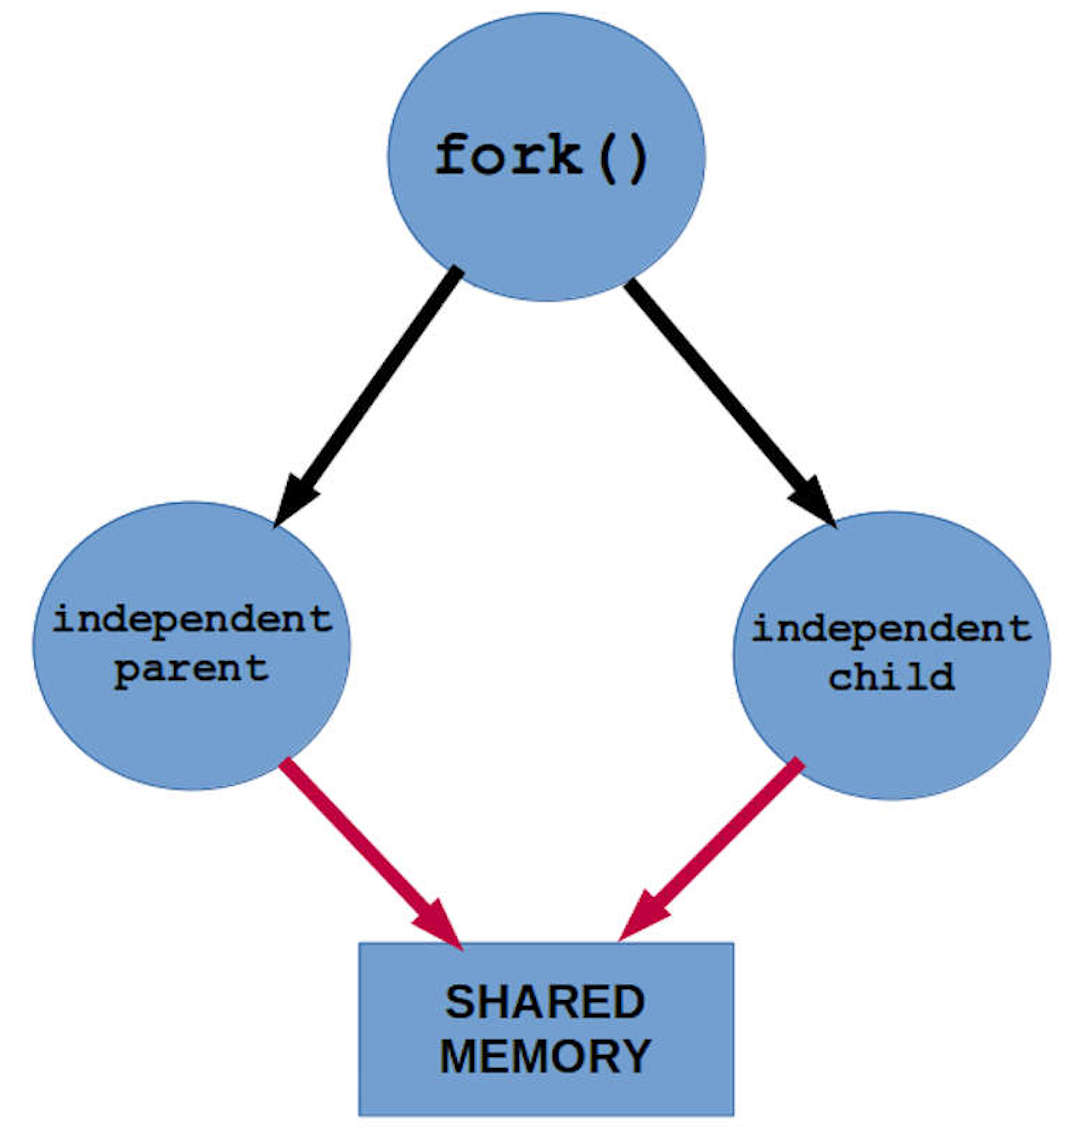
\includegraphics[width=0.28\linewidth]{os-concurrecy}
\caption{Concurrency}
\end{figure}

\end{frame}

% XXXXXXXXXXXXXXXXXXXXXXXXXXXXXXXXXXXXXXXXXXXXXXXXXXXXXXXXXXXXXXXXXXXXXXXXXX

\begin{frame}[fragile]
\frametitle{Race Condition}

\begin{itemize}
\item Critical Section
\end{itemize}

\begin{figure}
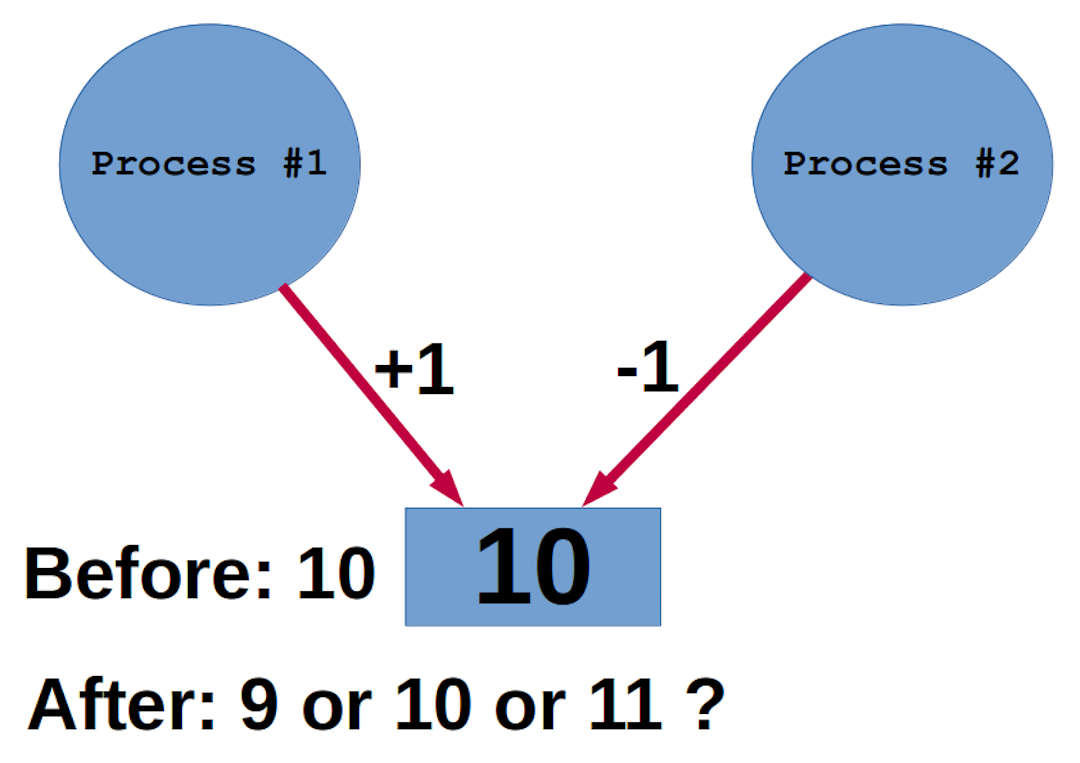
\includegraphics[width=0.56\linewidth]{os-critical}
\caption{Race Condition}
\end{figure}

\end{frame}

% XXXXXXXXXXXXXXXXXXXXXXXXXXXXXXXXXXXXXXXXXXXXXXXXXXXXXXXXXXXXXXXXXXXXXXXXXX

\section{The Critical Section Problem}
\begin{frame}
\frametitle{The Critical Section Problem}
\begin{itemize}
\item Requirements with nonzero speed assumption:
\begin{itemize}
\item Mutual Exclusion
\item Progress
\item Bounded Waiting
\end{itemize}
\item Peterson's Solution
\item Semaphores
\item Classical Problems
\begin{itemize}
\item Bounded-Buffer Problem
\item Readers and Writers Problem
\item Dining-Philosophers Problem
\end{itemize}

\item Resource and Allocation Graph

\end{itemize}

\begin{figure}
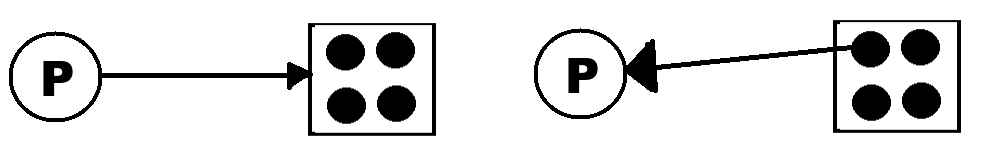
\includegraphics[width=0.60\linewidth]{os07-graph}
\caption{Request and Holding}
\end{figure}

\end{frame}

% XXXXXXXXXXXXXXXXXXXXXXXXXXXXXXXXXXXXXXXXXXXXXXXXXXXXXXXXXXXXXXXXXXXXXXXXXX
\section{Peterson}
\begin{frame}
\frametitle{Peterson's Solution}
\begin{tabular}{l  l}
\textbf{Process 0} &
\textbf{Process 1} \\
&\\
\multicolumn{2}{l}{
\hspace{10pt}
\texttt{flag[0]=} 
\hspace{60pt}
\texttt{turn=}
\hspace{20pt}
\texttt{flag[1]=} 
} \\
&\\
\texttt{do \{} & 
\texttt{do \{} \\
\hspace{18pt}\texttt{flag[0] = true} &
\hspace{18pt}\texttt{flag[1] = true} \\
\hspace{18pt}\texttt{turn = 1} &
\hspace{18pt}\texttt{turn = 0} \\
\hspace{18pt}{while (flag[1] \&\& turn == 1)} &
\hspace{18pt}{while (flag[0] \&\& turn == 0)} \\
\hspace{28pt}\texttt{(do nothing);} &
\hspace{28pt}\texttt{(do nothing);} \\
\hspace{18pt}\textbf{[CRITICAL SECTION];} &
\hspace{18pt}\textbf{[CRITICAL SECTION];} \\
\hspace{18pt}\texttt{flag[0] = false} &
\hspace{18pt}\texttt{flag[1] = false} \\
\hspace{18pt}\textbf{[REMAINDER SECTION];} &
\hspace{18pt}\textbf{[REMAINDER SECTION];} \\
\texttt{\} while(true);} &
\texttt{\} while(true);} \\
\end{tabular}
\end{frame}

% XXXXXXXXXXXXXXXXXXXXXXXXXXXXXXXXXXXXXXXXXXXXXXXXXXXXXXXXXXXXXXXXXXXXXXXXXX

\section{Semaphore}
\begin{frame}[fragile]
\frametitle{Semaphore}
\begin{itemize}
\item Dijkstra's Seinpalen (1963): Probeer (Try) en Verhoog (+1)
\item Semaphore:
\begin{itemize}
\item Wait(W) and Signal(S)
\item Atomic Operation
\end{itemize}
\item Linux System Calls: \texttt{sem\_init(), sem\_wait(), and sem\_post()}
\end{itemize}

\begin{lstlisting}[basicstyle=\ttfamily\footnotesize]

# Semaphore (Seinpalen)
# Wait (Probeer)
wait(S) {
   while (S <= 0)
      ; // busy wait
   S--;
}

# Signal (Verhoog)
signal(S) {
   S++;
}

\end{lstlisting}

\end{frame}

% XXXXXXXXXXXXXXXXXXXXXXXXXXXXXXXXXXXXXXXXXXXXXXXXXXXXXXXXXXXXXXXXXXXXXXXXXX

\section{Deadlock and Starvation}
\begin{frame}[fragile]
\frametitle{Deadlock and Starvation}

\begin{itemize}
\item Deadlock Characterization
\begin{itemize}
\item Mutual exclusion
\item Hold and wait
\item No preemption
\item Circular wait
\end{itemize}

\item Banker's Algorithm

\item Deadlock Prevention

\item Deadlock Avoidence

\item How do Operating Systems handle Deadlocks?
\\ [3mm]

\begin{tabular}{|l|}
\hline
\textbf{IGNORE THE PROBLEM!}\\
Pretending that deadlocks never occur \\
Just \textbf{RESET/REBOOT} it\\
This is how they \textbf{DO IT}! \\
\hline
\end{tabular}

\end{itemize}
\end{frame}

% 14 XXXXXXXXXXXXXXXXXXXXXXXXXXXXXXXXXXXXXXXXXXXXXXXXXXXXXXXXXXXXXXXXXXXXXXX

\begin{frame}[fragile]
\frametitle{setuid, setgid, sticky bit}

\begin{figure}
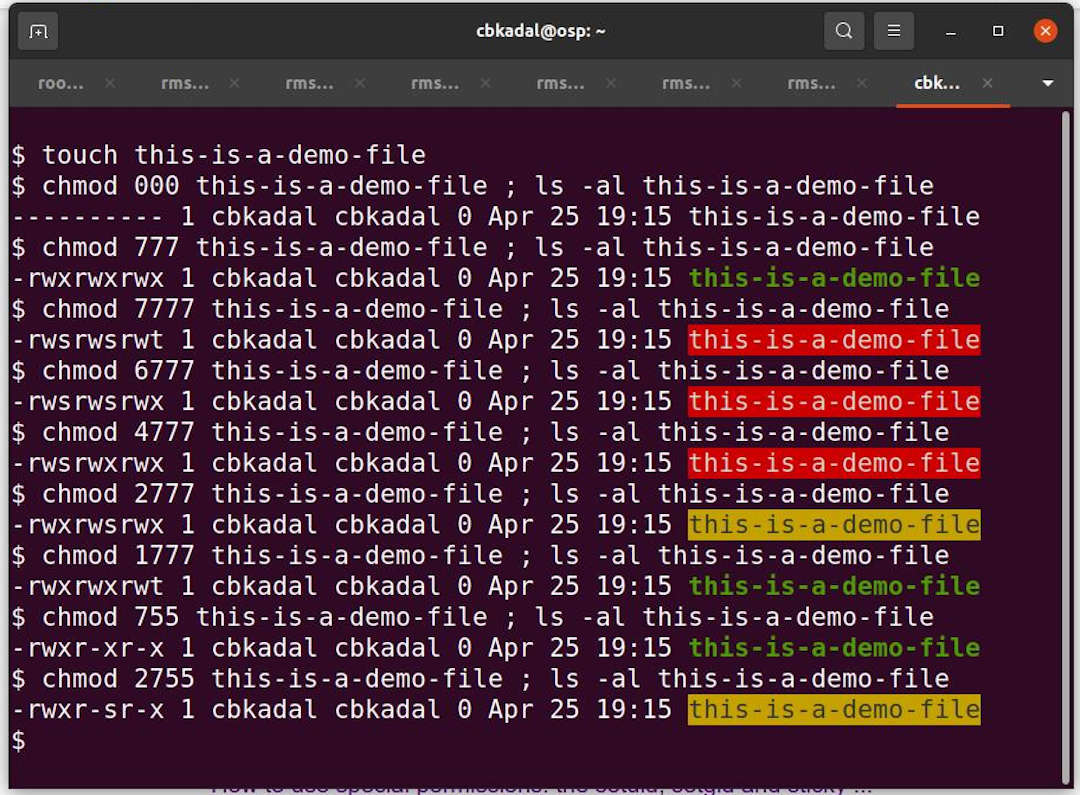
\includegraphics[width=0.60\linewidth]{os-set-ug-id}
\caption{setuid, setgid, sticky bit}
\end{figure}

\end{frame}


% XXXXXXXXXXXXXXXXXXXXXXXXXXXXXXXXXXXXXXXXXXXXXXXXXXXXXXXXXXXXXXXXXXXXXXXXXX
\section{99-myutils.h}
\begin{frame}[fragile]
\frametitle{99-myutils.h (01)}
% \begin{lstlisting}[basicstyle=\ttfamily\tiny]         % 108
\begin{lstlisting}[basicstyle=\ttfamily\footnotesize] %  72
% \begin{lstlisting}[basicstyle=\ttfamily\small]        %  65
% \begin{lstlisting}[basicstyle=\ttfamily\large]        %  54

/* (c) 2011-2018 Rahmat M. Samik-Ibrahim -- This is free software
 * Feel free to copy and/or modify and/or distribute it, 
 * provided this notice, and the copyright notice, are preserved. 
 * REV04 Wed Aug 29 18:47:14 WIB 2018 */

#include <semaphore.h>
#define MAX_THREAD 256
#define MAX_globalID 5
#define BUFFER_SIZE  5
#define TRUE         1
#define FALSE        0

extern sem_t    mutex, db, empty, full, globalIDmutex;
typedef struct {
   int   buffer[BUFFER_SIZE];
   int   in;
   int   out;
   int   count;
} bbuf_t;

\end{lstlisting}
\end{frame}

% XXXXXXXXXXXXXXXXXXXXXXXXXXXXXXXXXXXXXXXXXXXXXXXXXXXXXXXXXXXXXXXXXXXXXXXXXX
\begin{frame}[fragile]
\frametitle{99-myutils.h (02)}
% \begin{lstlisting}[basicstyle=\ttfamily\tiny]         % 108
\begin{lstlisting}[basicstyle=\ttfamily\footnotesize] %  72
% \begin{lstlisting}[basicstyle=\ttfamily\small]        %  65
% \begin{lstlisting}[basicstyle=\ttfamily\large]        %  54

void daftar_trit   (void* trit);      // mempersiapkan "trit"
void jalankan_trit (void);            // menjalankan dan menunggu hasil 
                                      // dari "daftar_trit"
void beberes_trit  (char* pesan);     // beberes menutup "jalankan_trit"

void rehat_acak  (long max_mdetik);  //istirohat acak "0-max_mdetik"(ms)

void init_globalID (void);            // globalID
int getADDglobalID (int id);          // globalID[id]++

void init_buffer   (void);            // init buffer
void enter_buffer  (int entry);       // enter  an integer item 
int remove_buffer  (void);            // remove the item

void init_rw       (void);            // init readers writers
int  startRead     (void);            // start reading
int  endRead       (void);            // end reading
void startWrite    (void);            // start writing
void endWrite      (void);            // end writing

\end{lstlisting}
\end{frame}

% XXXXXXXXXXXXXXXXXXXXXXXXXXXXXXXXXXXXXXXXXXXXXXXXXXXXXXXXXXXXXXXXXXXXXXXXXX
\section{99-myutils.c}
\begin{frame}[fragile]
\frametitle{99-myutils.c (01)}
% \begin{lstlisting}[basicstyle=\ttfamily\tiny]         % 108
\begin{lstlisting}[basicstyle=\ttfamily\footnotesize] %  72
% \begin{lstlisting}[basicstyle=\ttfamily\small]        %  65
% \begin{lstlisting}[basicstyle=\ttfamily\large]        %  54

/*
 * (c) 2011-2020 Rahmat M. Samik-Ibrahim -- This is free software
 * Feel free to copy and/or modify and/or distribute it, 
 * provided this notice, and the copyright notice, are preserved. 
 * REV04 Wed Mar 25 08:58:08 WIB 2020
 * REV03 Wed Aug 29 18:46:36 WIB 2018
 * REV02 Tue Nov  7 20:15:16 WIB 2017
 * REV01 Wed Nov  2 11:49:55 WIB 2016
 * START Xxx Mar 30 02:13:01 UTC 2011
 */

#include <pthread.h>
#include <stdio.h>
#include <stdlib.h>
#include <time.h>
#include "99-myutils.h"

sem_t    mutex, db, empty, full, globalIDmutex;

\end{lstlisting}
\end{frame}

% XXXXXXXXXXXXXXXXXXXXXXXXXXXXXXXXXXXXXXXXXXXXXXXXXXXXXXXXXXXXXXXXXXXXXXXXXX
\begin{frame}[fragile]
\frametitle{99-myutils.c (02)}
\begin{lstlisting}[basicstyle=\ttfamily\tiny]         % 108
% \begin{lstlisting}[basicstyle=\ttfamily\footnotesize] %  72
% \begin{lstlisting}[basicstyle=\ttfamily\small]        %  65
% \begin{lstlisting}[basicstyle=\ttfamily\large]        %  54

/* TRIT ***************************************************/
int       jumlah_trit = 0;
void*     trits  [MAX_THREAD];
pthread_t trit_id[MAX_THREAD];
void daftar_trit(void *trit) {
   if(jumlah_trit >= MAX_THREAD) {
      printf("\n ERROR MAX daftar_trit %d\n",jumlah_trit);
      exit(1);
   }
   trits[jumlah_trit++] = trit;
}
void jalankan_trit(void){
   int ii;
   for (ii=0;ii<jumlah_trit;ii++) {
      if(pthread_create(&trit_id[ii], NULL, trits[ii], NULL)) {
         printf("\n ERROR pthread_creat: %d\n",ii);
         exit(1);
      }
   }
   for (ii=0;ii<jumlah_trit;ii++){
      if(pthread_join(trit_id[ii], NULL)) {
         printf("\n ERROR pthread_join: %d\n",ii);
         exit(1);
      }
   }
}
void beberes_trit(char* pesan) {
   if (pesan != NULL) printf("%s\n",pesan);
   pthread_exit(NULL);
}

\end{lstlisting}
\end{frame}

% XXXXXXXXXXXXXXXXXXXXXXXXXXXXXXXXXXXXXXXXXXXXXXXXXXXXXXXXXXXXXXXXXXXXXXXXXX
\begin{frame}[fragile]
\frametitle{99-myutils.c (03)}
% \begin{lstlisting}[basicstyle=\ttfamily\tiny]         % 108
% \begin{lstlisting}[basicstyle=\ttfamily\footnotesize] %  72
\begin{lstlisting}[basicstyle=\ttfamily\small]        %  65
% \begin{lstlisting}[basicstyle=\ttfamily\large]        %  54

/* REHAT **********************************************/
int  pertamax    = TRUE;

void rehat_acak(long max_mdetik) {
   struct timespec tim;
   long            ndetik;
  
   if (pertamax) {
      pertamax = FALSE;
      srandom((unsigned int) time (NULL));
   }
   ndetik      = random() % max_mdetik;
   tim.tv_sec  = ndetik   / 1000L;
   tim.tv_nsec = ndetik   % 1000L * 1000000L;
   nanosleep(&tim,NULL);
} 

\end{lstlisting}
\end{frame}

% XXXXXXXXXXXXXXXXXXXXXXXXXXXXXXXXXXXXXXXXXXXXXXXXXXXXXXXXXXXXXXXXXXXXXXXXXX
\begin{frame}[fragile]
\frametitle{99-myutils.c (04)}
% \begin{lstlisting}[basicstyle=\ttfamily\tiny]         % 108
% \begin{lstlisting}[basicstyle=\ttfamily\footnotesize] %  72
\begin{lstlisting}[basicstyle=\ttfamily\small]        %  65
% \begin{lstlisting}[basicstyle=\ttfamily\large]        %  54

/* globalID ********************************************* */

int globalID[MAX_globalID];

void init_globalID (void) {
   sem_init (&globalIDmutex, 0, 1);
   for (int ii=0; ii<MAX_globalID; ii++) {
      globalID[ii]=0;
   }
}

int getADDglobalID (int id) {
   sem_wait (&globalIDmutex);
   int ii=globalID[id]++;
   sem_post (&globalIDmutex);
   return ii;
}

\end{lstlisting}
\end{frame}

% XXXXXXXXXXXXXXXXXXXXXXXXXXXXXXXXXXXXXXXXXXXXXXXXXXXXXXXXXXXXXXXXXXXXXXXXXX
\begin{frame}[fragile]
\frametitle{99-myutils.c (05)}
% \begin{lstlisting}[basicstyle=\ttfamily\tiny]         % 108
% \begin{lstlisting}[basicstyle=\ttfamily\footnotesize] %  72
% \begin{lstlisting}[basicstyle=\ttfamily\small]        %  65
\begin{lstlisting}[basicstyle=\ttfamily\large]        %  54

/* BOUNDED BUFFER *********************************/

bbuf_t buf;

void init_buffer(void) {
   buf.in    = 0;
   buf.out   = 0;
   buf.count = 0;
   sem_init   (&mutex, 0, 1);
   sem_init   (&empty, 0, BUFFER_SIZE);
   sem_init   (&full,  0, 0);
}

\end{lstlisting}
\end{frame}

% XXXXXXXXXXXXXXXXXXXXXXXXXXXXXXXXXXXXXXXXXXXXXXXXXXXXXXXXXXXXXXXXXXXXXXXXXX
\begin{frame}[fragile]
\frametitle{99-myutils.c (06)}
% \begin{lstlisting}[basicstyle=\ttfamily\tiny]         % 108
\begin{lstlisting}[basicstyle=\ttfamily\footnotesize] %  72
% \begin{lstlisting}[basicstyle=\ttfamily\small]        %  65
% \begin{lstlisting}[basicstyle=\ttfamily\large]        %  54
void enter_buffer(int entry) {
   sem_wait(&empty);
   sem_wait(&mutex);
   buf.count++;
   buf.buffer[buf.in] = entry;
   buf.in = (buf.in+1) % BUFFER_SIZE;
   sem_post(&mutex);
   sem_post(&full);
}
int remove_buffer(void) {
   int item;
   sem_wait(&full);
   sem_wait(&mutex);
   buf.count--;
   item = buf.buffer[buf.out];
   buf.out = (buf.out+1) % BUFFER_SIZE;
   sem_post(&mutex);
   sem_post(&empty);
   return item;
}

\end{lstlisting}
\end{frame}

% XXXXXXXXXXXXXXXXXXXXXXXXXXXXXXXXXXXXXXXXXXXXXXXXXXXXXXXXXXXXXXXXXXXXXXXXXX
\begin{frame}[fragile]
\frametitle{99-myutils.c (07)}
% \begin{lstlisting}[basicstyle=\ttfamily\tiny]         % 108
% \begin{lstlisting}[basicstyle=\ttfamily\footnotesize] %  72
% \begin{lstlisting}[basicstyle=\ttfamily\small]        %  65
\begin{lstlisting}[basicstyle=\ttfamily\large]        %  54

/* READERS WRITERS ***********************/
int readerCount;
void init_rw(void) {
   readerCount = 0;
   sem_init   (&mutex,  0, 1);
   sem_init   (&db,     0, 1);
}
int startRead(void) {
   sem_wait(&mutex);
   if (++readerCount == 1 )
      sem_wait(&db);
   sem_post(&mutex);
   return readerCount;
} 

\end{lstlisting}
\end{frame}

% XXXXXXXXXXXXXXXXXXXXXXXXXXXXXXXXXXXXXXXXXXXXXXXXXXXXXXXXXXXXXXXXXXXXXXXXXX
\begin{frame}[fragile]
\frametitle{99-myutils.c (08)}
% \begin{lstlisting}[basicstyle=\ttfamily\tiny]         % 108
% \begin{lstlisting}[basicstyle=\ttfamily\footnotesize] %  72
% \begin{lstlisting}[basicstyle=\ttfamily\small]        %  65
\begin{lstlisting}[basicstyle=\ttfamily\large]        %  54

int endRead(void) {
   sem_wait(&mutex);
   if (--readerCount == 0 )
      sem_post(&db);
   sem_post(&mutex);
   return readerCount;
} 

void startWrite(void) {
   sem_wait(&db);
}

void endWrite(void) {
   sem_post(&db);
}

\end{lstlisting}
\end{frame}

% XXXXXXXXXXXXXXXXXXXXXXXXXXXXXXXXXXXXXXXXXXXXXXXXXXXXXXXXXXXXXXXXXXXXXXXXXX
\section{00-thread}
\begin{frame}[fragile]
\frametitle{00-thread (01)}
% \begin{lstlisting}[basicstyle=\ttfamily\tiny]         % 108
% \begin{lstlisting}[basicstyle=\ttfamily\footnotesize] %  72
\begin{lstlisting}[basicstyle=\ttfamily\small]        %  65
% \begin{lstlisting}[basicstyle=\ttfamily\large]        %  54

/*
 * Copyright (C) 2015-2020 Rahmat M. Samik-Ibrahim
 * http://rahmatm.samik-ibrahim.vlsm.org/
 * REV11 Tue Mar 24 17:03:47 WIB 2020
 * START Xxx Sep 30 XX:XX:XX UTC 2015
 */

#include <stdio.h>
#include <stdlib.h>
#include <unistd.h>
#include <sys/types.h>
#include "99-myutils.h"

volatile int loop  = 6; // display 6 times
volatile int share = 0; // start share=0

\end{lstlisting}
\end{frame}

% XXXXXXXXXXXXXXXXXXXXXXXXXXXXXXXXXXXXXXXXXXXXXXXXXXXXXXXXXXXXXXXXXXXXXXXXXX
\begin{frame}[fragile]
\frametitle{00-thread (02)}
% \begin{lstlisting}[basicstyle=\ttfamily\tiny]         % 108
% \begin{lstlisting}[basicstyle=\ttfamily\footnotesize] %  72
% \begin{lstlisting}[basicstyle=\ttfamily\small]        %  65
\begin{lstlisting}[basicstyle=\ttfamily\large]        %  54
// fflush() I/O before sleep() 
void  flushsleep(int ii) {
   fflush(NULL);
   sleep (ii  );
}
// THREAD#1: start share=1000 --> share++
void* thread1 (void* a) {
   printf("THREAD#1-PID[%5.5d]\n", getpid());
   flushsleep(1);
   rehat_acak(100);
   share = 1000;
   while (loop > 0) {
      rehat_acak(100);
      share++;
   }
}

\end{lstlisting}
\end{frame}

% XXXXXXXXXXXXXXXXXXXXXXXXXXXXXXXXXXXXXXXXXXXXXXXXXXXXXXXXXXXXXXXXXXXXXXXXXX
\begin{frame}[fragile]
\frametitle{00-thread (03)}
% \begin{lstlisting}[basicstyle=\ttfamily\tiny]         % 108
% \begin{lstlisting}[basicstyle=\ttfamily\footnotesize] %  72
% \begin{lstlisting}[basicstyle=\ttfamily\small]        %  65
\begin{lstlisting}[basicstyle=\ttfamily\large]        %  54

// THREAD#2: start share=2000 --> share--
void* thread2 (void* a) {
   printf("THREAD#2-PID[%5.5d]\n", getpid());
   flushsleep(1);
   rehat_acak(100);
   share = 2000;
   while (loop > 0) {
      rehat_acak(100);
      share--;
   }
}

\end{lstlisting}
\end{frame}

% XXXXXXXXXXXXXXXXXXXXXXXXXXXXXXXXXXXXXXXXXXXXXXXXXXXXXXXXXXXXXXXXXXXXXXXXXX
\begin{frame}[fragile]
\frametitle{00-thread (04)}
% \begin{lstlisting}[basicstyle=\ttfamily\tiny]         % 108
% \begin{lstlisting}[basicstyle=\ttfamily\footnotesize] %  72
\begin{lstlisting}[basicstyle=\ttfamily\small]        %  65
% \begin{lstlisting}[basicstyle=\ttfamily\large]        %  54

// THREAD#3: display "share" every 1 second
void* thread3 (void* a) {
   printf("THREAD#3-PID[%5.5d]\n", getpid());
   while (loop-- > 0) {
      printf("---SHARE----+%5.5d+\n", share);
      flushsleep(1);
   }
}
// MAIN: start share=0
void main(void) {
   printf("---MAIN--PID[%5.5d]\n", getpid());
   daftar_trit   (thread1);
   daftar_trit   (thread2);
   daftar_trit   (thread3);
   jalankan_trit ();
   beberes_trit  ("------------  Done.");
}

\end{lstlisting}
\end{frame}

% XXXXXXXXXXXXXXXXXXXXXXXXXXXXXXXXXXXXXXXXXXXXXXXXXXXXXXXXXXXXXXXXXXXXXXXXXX
\begin{frame}[fragile]
\frametitle{00-thread (05)}
\begin{lstlisting}[basicstyle=\ttfamily\tiny]         % 108
% \begin{lstlisting}[basicstyle=\ttfamily\footnotesize] %  72
% \begin{lstlisting}[basicstyle=\ttfamily\small]        %  65
% \begin{lstlisting}[basicstyle=\ttfamily\large]        %  54

$ ./00-thread 
---MAIN--PID[05568]
THREAD#1-PID[05568]
THREAD#2-PID[05568]
THREAD#3-PID[05568]
---SHARE----+00000+
---SHARE----+00000+
---SHARE----+02001+
---SHARE----+02001+
---SHARE----+02000+
---SHARE----+01995+
------------  Done.

$ ./00-thread 
---MAIN--PID[05576]
THREAD#1-PID[05576]
THREAD#2-PID[05576]
THREAD#3-PID[05576]
---SHARE----+00000+
---SHARE----+00000+
---SHARE----+01001+
---SHARE----+01006+
---SHARE----+01006+
---SHARE----+01005+
------------  Done.

\end{lstlisting}
\end{frame}

% XXXXXXXXXXXXXXXXXXXXXXXXXXXXXXXXXXXXXXXXXXXXXXXXXXXXXXXXXXXXXXXXXXXXXXXXXX
\section{01-thread}
\begin{frame}[fragile]
\frametitle{01-thread (01)}
\begin{lstlisting}[basicstyle=\ttfamily\footnotesize]

>>>>> $ cat 01-thread.c
/*
 * (c) 2015-2017 Rahmat M. Samik-Ibrahim
 * https://rahmatm.samik-ibrahim.vlsm.org/
 * This is free software.
 * REV02 Wed Nov  1 16:48:40 WIB 2017
 * REV01 Wed Nov  2 11:49:39 WIB 2016
 * START Xxx Sep 30 XX:XX:XX UTC 2015
 */

#include <stdio.h>
#include <stdlib.h>
#include <semaphore.h>
#include "99-myutils.h"

sem_t	generik;
sem_t	generik2;

\end{lstlisting}
\end{frame}

% XXXXXXXXXXXXXXXXXXXXXXXXXXXXXXXXXXXXXXXXXXXXXXXXXXXXXXXXXXXXXXXXXXXXXXXXXX
\begin{frame}[fragile]
\frametitle{01-thread (02)}
\begin{lstlisting}[basicstyle=\ttfamily\tiny]
void* thread1 (void* a) {
   sem_wait   (&generik);
   printf("THREAD1: I am second!\n");
   sem_post   (&generik2);
}
void* thread2 (void* a) {
   printf("THREAD2: I am first!\n");
   sem_post   (&generik);
}

void* thread3 (void* a) {
   sem_wait   (&generik2);
   printf("THREAD3: I am last!\n");
}

void main(void) {
   sem_init      (&generik,  0, 0);
   sem_init      (&generik2, 0, 0);
   daftar_trit   (thread1);
   daftar_trit   (thread2);
   daftar_trit   (thread3);
   jalankan_trit ();
   beberes_trit  ("Bye Bye Main...");
}

>>>>> $ 01-thread 
THREAD2: I am first!
THREAD1: I am second!
THREAD3: I am last!
Bye Bye Main...

\end{lstlisting}
\end{frame}

% XXXXXXXXXXXXXXXXXXXXXXXXXXXXXXXXXXXXXXXXXXXXXXXXXXXXXXXXXXXXXXXXXXXXXXXXXX
\section{02-prodkon}
\begin{frame}[fragile]
\frametitle{02-prodkon (01)}
% \begin{lstlisting}[basicstyle=\ttfamily\tiny]         % 108
% \begin{lstlisting}[basicstyle=\ttfamily\footnotesize] %  72
% \begin{lstlisting}[basicstyle=\ttfamily\small]        %  65
% \begin{lstlisting}[basicstyle=\ttfamily\large]        %  54
\begin{lstlisting}[basicstyle=\ttfamily\tiny]

/*
 * Copyright (C) 2011-2020 Rahmat M. Samik-Ibrahim
 * http://rahmatm.samik-ibrahim.vlsm.org/
 * This program is free script/software. This program is distributed in the 
 * hope that it will be useful, but WITHOUT ANY WARRANTY; without even the 
 * implied warranty of MERCHANTABILITY or FITNESS FOR A PARTICULAR PURPOSE.
 * REV06 Tue Mar 24 17:11:58 WIB 2020
 * REV05 Wed Aug 29 18:35:33 WIB 2018
 * REV04 Tue Apr 17 09:31:37 WIB 2018
 * START Xxx Mar 30 02:13:01 UTC 2011
 */

#include <stdio.h>
#include <stdlib.h>
#include "99-myutils.h"

#define P_REHAT 1000
#define K_REHAT 3000
int produk = 0;

void* Produsen (void* a) {
   printf("Produsen siap...\n");
   while (TRUE) {
      printf("P: REHAT ******\n");
      rehat_acak(P_REHAT);
      printf("P: PRODUKSI %d\n", produk);
      enter_buffer  (produk++);
   }
}

\end{lstlisting}
\end{frame}

% XXXXXXXXXXXXXXXXXXXXXXXXXXXXXXXXXXXXXXXXXXXXXXXXXXXXXXXXXXXXXXXXXXXXXXXXXX
\begin{frame}[fragile]
\frametitle{02-prodkon (02)}
% \begin{lstlisting}[basicstyle=\ttfamily\tiny]         % 108
% \begin{lstlisting}[basicstyle=\ttfamily\footnotesize] %  72
% \begin{lstlisting}[basicstyle=\ttfamily\small]        %  65
% \begin{lstlisting}[basicstyle=\ttfamily\large]        %  54
\begin{lstlisting}[basicstyle=\ttfamily\tiny]
void* Konsumen (void* a) {
   printf   ("                        Konsumen siap...\n");
   while (TRUE) {
      printf("                        K: REHAT ******\n");
      rehat_acak(K_REHAT);
      printf("                        K: KONSUMSI %d\n", remove_buffer());
   }
}
int main(int argc, char * argv[])
{
   init_buffer();
   daftar_trit(Produsen);
   daftar_trit(Konsumen);
   jalankan_trit();
   beberes_trit("Selese...");
}
##################
>>>>> $ ./02-prodkon 
Produsen siap...
P: REHAT ******
                        Konsumen siap...
                        K: REHAT ******
P: PRODUKSI 0
P: REHAT ******
                        K: KONSUMSI 0
                        K: REHAT ******
P: PRODUKSI 1
P: REHAT ******
P: PRODUKSI 2
P: REHAT ******

\end{lstlisting}
\end{frame}

% XXXXXXXXXXXXXXXXXXXXXXXXXXXXXXXXXXXXXXXXXXXXXXXXXXXXXXXXXXXXXXXXXXXXXXXXXX
\section{03-readwrite}
\begin{frame}[fragile]
\frametitle{03-readwrite (01)}
% \begin{lstlisting}[basicstyle=\ttfamily\tiny]         % 108
% \begin{lstlisting}[basicstyle=\ttfamily\footnotesize] %  72
% \begin{lstlisting}[basicstyle=\ttfamily\small]        %  65
% \begin{lstlisting}[basicstyle=\ttfamily\large]        %  54
\begin{lstlisting}[basicstyle=\ttfamily\tiny]

>>>>> $ cat 03-readwrite.c

/*
 * (c) 2011-2017 Rahmat M. Samik-Ibrahim
 * https://rahmatm.samik-ibrahim.vlsm.org/
 * This is free software.
 * REV02 Wed Nov  1 16:53:38 WIB 2017
 * REV01 Wed Nov  2 13:49:55 WIB 2016
 * REV00 Xxx Sep 30 XX:XX:XX UTC 2015
 * START Xxx Mar 30 02:13:01 UTC 2011
 */

#include <stdio.h>
#include <stdlib.h>
#include <semaphore.h>
#include "99-myutils.h"

extern sem_t    mutex, db, empty, full, rmutex, wmutex;

#define R_REHAT 4000
#define R_READ  4000
#define R_JUMLAH   4

#define W_REHAT 2000
#define W_WRITE 2000
#define W_JUMLAH   3

int reader_ID = 0;
int writer_ID = 0;

\end{lstlisting}
\end{frame}

% XXXXXXXXXXXXXXXXXXXXXXXXXXXXXXXXXXXXXXXXXXXXXXXXXXXXXXXXXXXXXXXXXXXXXXXXXX
\begin{frame}[fragile]
\frametitle{03-readwrite (02)}
% \begin{lstlisting}[basicstyle=\ttfamily\tiny]
% \begin{lstlisting}[basicstyle=\ttfamily\small]
% \begin{lstlisting}[basicstyle=\ttfamily\large]
\begin{lstlisting}[basicstyle=\ttfamily\footnotesize]
void* Reader (void* a) {
   int  my_ID;

   sem_wait (&rmutex);
   my_ID  = reader_ID++;
   sem_post (&rmutex);

   printf   ("               READER %d: SIAP  ******\n", my_ID);
   while (TRUE) {
      printf("               READER %d: REHAT ******\n", my_ID);
      rehat_acak(R_REHAT);
      printf("               READER %d: MAU  MEMBACA\n", my_ID);
      printf("               **** JUMLAH PEMBACA %d\n", startRead());
      printf("               READER %d:=SEDANG==BACA\n", my_ID);
      rehat_acak(R_READ);
      printf("               READER %d: SELESAI BACA\n", my_ID);
      printf("               **** SISA PEMBACA %d\n", endRead());
   }
}

\end{lstlisting}
\end{frame}

% XXXXXXXXXXXXXXXXXXXXXXXXXXXXXXXXXXXXXXXXXXXXXXXXXXXXXXXXXXXXXXXXXXXXXXXXXX
\begin{frame}[fragile]
\frametitle{03-readwrite (03)}
% \begin{lstlisting}[basicstyle=\ttfamily\tiny]         % 108
% \begin{lstlisting}[basicstyle=\ttfamily\footnotesize] %  72
% \begin{lstlisting}[basicstyle=\ttfamily\small]        %  65
% \begin{lstlisting}[basicstyle=\ttfamily\large]        %  54
\begin{lstlisting}[basicstyle=\ttfamily\tiny]

void* Writer (void* a) {
   int  my_ID;

   sem_wait (&wmutex);
   my_ID  = writer_ID++;
   sem_post (&wmutex);
   printf   ("WRITER %d: SIAP  *******\n", my_ID);
   while (TRUE) {
      printf("WRITER %d: REHAT *******\n", my_ID);
      rehat_acak(W_REHAT);
      printf("WRITER %d: MAU   MENULIS\n", my_ID);
      startWrite();
      printf("WRITER %d:=SEDANG==NULIS\n", my_ID);
      rehat_acak(W_WRITE);
      endWrite();
      printf("WRITER %d: SELESAI NULIS\n", my_ID);
   }
}
int main(int argc, char * argv[])
{
   int ii;
   init_rw();
   for (ii = 0 ; ii < R_JUMLAH; ii++)
      daftar_trit(Reader);
   for (ii = 0 ; ii < W_JUMLAH; ii++)
      daftar_trit(Writer);
   jalankan_trit();
   beberes_trit("Selese...");
}

\end{lstlisting}
\end{frame}

% XXXXXXXXXXXXXXXXXXXXXXXXXXXXXXXXXXXXXXXXXXXXXXXXXXXXXXXXXXXXXXXXXXXXXXXXXX
\begin{frame}[fragile]
\frametitle{03-readwrite (04)}
% \begin{lstlisting}[basicstyle=\ttfamily\tiny]         % 108
% \begin{lstlisting}[basicstyle=\ttfamily\footnotesize] %  72
% \begin{lstlisting}[basicstyle=\ttfamily\small]        %  65
% \begin{lstlisting}[basicstyle=\ttfamily\large]        %  54
\begin{lstlisting}[basicstyle=\ttfamily\tiny]
>>>>> $ 03-readwrite 
                        READER 1: SIAP  ******
                        READER 1: REHAT ******
                        READER 0: SIAP  ******
                        READER 0: REHAT ******
WRITER 1: SIAP  *******
WRITER 1: REHAT *******
                        READER 3: SIAP  ******
                        READER 3: REHAT ******
                        READER 2: SIAP  ******
                        READER 2: REHAT ******
WRITER 2: SIAP  *******
WRITER 2: REHAT *******
WRITER 0: SIAP  *******
WRITER 0: REHAT *******
WRITER 2: MAU   MENULIS
WRITER 2:=SEDANG==NULIS
                        READER 3: MAU  MEMBACA
                        READER 1: MAU  MEMBACA
WRITER 2: SELESAI NULIS
WRITER 2: REHAT *******
                        ***** JUMLAH PEMBACA 2
                        READER 1:=SEDANG==BACA
                        ***** JUMLAH PEMBACA 1
                        READER 3:=SEDANG==BACA
WRITER 1: MAU   MENULIS
                        READER 1: SELESAI BACA
                        ***** SISA PEMBACA 1
                        READER 1: REHAT ******
WRITER 0: MAU   MENULIS
                        READER 3: SELESAI BACA

\end{lstlisting}
\end{frame}

% XXXXXXXXXXXXXXXXXXXXXXXXXXXXXXXXXXXXXXXXXXXXXXXXXXXXXXXXXXXXXXXXXXXXXXXXXX
\section{04-readwrite}
\begin{frame}[fragile]
\frametitle{04-readwrite (01)}
% \begin{lstlisting}[basicstyle=\ttfamily\tiny]         % 108
\begin{lstlisting}[basicstyle=\ttfamily\footnotesize] %  72
% \begin{lstlisting}[basicstyle=\ttfamily\small]        %  65
% \begin{lstlisting}[basicstyle=\ttfamily\large]        %  54

/* Copyright (C) 2011-2020 Rahmat M. Samik-Ibrahim
 * http://rahmatm.samik-ibrahim.vlsm.org/
 * This program is free script/software. 
 * REV08 Tue Mar 24 17:41:12 WIB 2020
 * START Xxx Mar 30 02:13:01 UTC 2011
 */

#include <stdio.h>
#include <stdlib.h>
#include "99-myutils.h"

sem_t           sync_er, sync_re, sync_ew, sync_we;

#define R_REHAT 1500
#define R_READ  1500
#define R_JUMLAH  2

#define W_REHAT 1500
#define W_WRITE 1500
#define W_JUMLAH  2

\end{lstlisting}
\end{frame}

% XXXXXXXXXXXXXXXXXXXXXXXXXXXXXXXXXXXXXXXXXXXXXXXXXXXXXXXXXXXXXXXXXXXXXXXXXX
\begin{frame}[fragile]
\frametitle{04-readwrite (02)}
% \begin{lstlisting}[basicstyle=\ttfamily\tiny]         % 108
% \begin{lstlisting}[basicstyle=\ttfamily\footnotesize] %  72
% \begin{lstlisting}[basicstyle=\ttfamily\small]        %  65
\begin{lstlisting}[basicstyle=\ttfamily\large]        %  54

#define aReader 0
#define aWriter 1
void* Extra (void* a) {
   int ii;
   while (TRUE) {
      for (ii=0; ii<W_JUMLAH; ii++)
         sem_wait (&sync_we);
      for (ii=0; ii<R_JUMLAH; ii++)
         sem_post (&sync_er);
      for (ii=0; ii<R_JUMLAH; ii++)
         sem_wait (&sync_re);
      for (ii=0; ii<W_JUMLAH; ii++)
         sem_post (&sync_ew);
   }
}

\end{lstlisting}
\end{frame}

% XXXXXXXXXXXXXXXXXXXXXXXXXXXXXXXXXXXXXXXXXXXXXXXXXXXXXXXXXXXXXXXXXXXXXXXXXX
\begin{frame}[fragile]
\frametitle{04-readwrite (03)}
% \begin{lstlisting}[basicstyle=\ttfamily\tiny]         % 108
\begin{lstlisting}[basicstyle=\ttfamily\footnotesize] %  72
% \begin{lstlisting}[basicstyle=\ttfamily\small]        %  65
% \begin{lstlisting}[basicstyle=\ttfamily\large]        %  54

void* Reader (void* a) {
   int  my_ID;
   sem_wait (&rmutex);
   my_ID  = reader_ID++;
   sem_post (&rmutex);
   printf   ("                  READER %d: SIAP  ******\n", my_ID);
   while (TRUE) {
      sem_wait (&sync_er);
      printf("                  READER %d: REHAT ******\n", my_ID);
      rehat_acak(R_REHAT);
      printf("                  READER %d: MAU  MEMBACA\n", my_ID);
      printf("             **** JUMLAH PEMBACA %d\n", startRead());
      printf("                  READER %d:=SEDANG==BACA\n", my_ID);
      rehat_acak(R_READ);
      printf("                  READER %d: SELESAI BACA\n", my_ID);
      printf("                ***** SISA PEMBACA %d\n", endRead());
      sem_post (&sync_re);
   }
}

\end{lstlisting}
\end{frame}

% XXXXXXXXXXXXXXXXXXXXXXXXXXXXXXXXXXXXXXXXXXXXXXXXXXXXXXXXXXXXXXXXXXXXXXXXXX
\begin{frame}[fragile]
\frametitle{04-readwrite (04)}
% \begin{lstlisting}[basicstyle=\ttfamily\tiny]         % 108
\begin{lstlisting}[basicstyle=\ttfamily\footnotesize] %  72
% \begin{lstlisting}[basicstyle=\ttfamily\small]        %  65
% \begin{lstlisting}[basicstyle=\ttfamily\large]        %  54

void* Writer (void* a) {
   int  my_ID;
   sem_wait (&wmutex);
   my_ID  = writer_ID++;
   sem_post (&wmutex);
   printf   ("WRITER %d: SIAP  *******\n", my_ID);
   while (TRUE) {
      printf("WRITER %d: REHAT *******\n", my_ID);
      rehat_acak(W_REHAT);
      printf("WRITER %d: MAU   MENULIS\n", my_ID);
      startWrite();
      printf("WRITER %d:=SEDANG==NULIS\n", my_ID);
      rehat_acak(W_WRITE);
      endWrite();
      printf("WRITER %d: SELESAI NULIS\n", my_ID);
      sem_post (&sync_we);
      sem_wait (&sync_ew);
   }
}

\end{lstlisting}
\end{frame}

% XXXXXXXXXXXXXXXXXXXXXXXXXXXXXXXXXXXXXXXXXXXXXXXXXXXXXXXXXXXXXXXXXXXXXXXXXX
\begin{frame}[fragile]
\frametitle{04-readwrite (05)}
% \begin{lstlisting}[basicstyle=\ttfamily\tiny]         % 108
\begin{lstlisting}[basicstyle=\ttfamily\footnotesize] %  72
% \begin{lstlisting}[basicstyle=\ttfamily\small]        %  65
% \begin{lstlisting}[basicstyle=\ttfamily\large]        %  54

int main(int argc, char * argv[])
{
   int ii;
   init_rw();
   sem_init   (&sync_er, 0, 0);
   sem_init   (&sync_re, 0, 0);
   sem_init   (&sync_ew, 0, 0);
   sem_init   (&sync_we, 0, 0);
   daftar_trit(Extra);
   for (ii = 0 ; ii < R_JUMLAH; ii++)
      daftar_trit(Reader);
   for (ii = 0 ; ii < W_JUMLAH; ii++)
      daftar_trit(Writer);
   jalankan_trit();
   beberes_trit("Selese...");
}

\end{lstlisting}
\end{frame}

% XXXXXXXXXXXXXXXXXXXXXXXXXXXXXXXXXXXXXXXXXXXXXXXXXXXXXXXXXXXXXXXXXXXXXXXXXX
\begin{frame}[fragile]
\frametitle{04-readwrite (06)}
% \begin{lstlisting}[basicstyle=\ttfamily\tiny]
% \begin{lstlisting}[basicstyle=\ttfamily\footnotesize] %
\begin{lstlisting}[basicstyle=\ttfamily\tiny]

>>>>> $ 04-readwrite 
                        READER 1: SIAP  ******
                        READER 0: SIAP  ******
WRITER 0: SIAP  *******
WRITER 0: REHAT *******
WRITER 1: SIAP  *******
WRITER 1: REHAT *******
WRITER 1: MAU   MENULIS
WRITER 1:=SEDANG==NULIS
WRITER 0: MAU   MENULIS
WRITER 0:=SEDANG==NULIS
WRITER 1: SELESAI NULIS
WRITER 0: SELESAI NULIS
                        READER 1: REHAT ******
                        READER 0: REHAT ******
                        READER 1: MAU  MEMBACA
                        ***** JUMLAH PEMBACA 1
                        READER 1:=SEDANG==BACA
                        READER 1: SELESAI BACA
                        ***** SISA PEMBACA 0
                        READER 0: MAU  MEMBACA
                        ***** JUMLAH PEMBACA 1
                        READER 0:=SEDANG==BACA
                        READER 0: SELESAI BACA
                        ***** SISA PEMBACA 0
WRITER 1: REHAT *******
WRITER 0: REHAT *******
WRITER 0: MAU   MENULIS
WRITER 0:=SEDANG==NULIS

\end{lstlisting}
\end{frame}

% XXXXXXXXXXXXXXXXXXXXXXXXXXXXXXXXXXXXXXXXXXXXXXXXXXXXXXXXXXXXXXXXXXXXXXXXXX
\section{05-alu}
\begin{frame}[fragile]
\frametitle{05-alu (01)}
% \begin{lstlisting}[basicstyle=\ttfamily\tiny]
% \begin{lstlisting}[basicstyle=\ttfamily\footnotesize] %
\begin{lstlisting}[basicstyle=\ttfamily\tiny]
>>>>> $ cat 05-alu.c
/* (c) 2013-2017 Rahmat M. Samik-Ibrahim
 * https://rahmatm.samik-ibrahim.vlsm.org/
 * This is free software.
 * REV02 Wed Nov  1 17:16:35 WIB 2017
 * REV01 Wed Nov  2 13:50:33 WIB 2016
 * START Xxx Xxx XX XX:XX:XX UTC 2013
 */

#include <stdio.h>
#include <stdlib.h>
#include <semaphore.h>
#include "99-myutils.h"
#define      NThreads 4
sem_t        mutex,   switch1, switch2;
int          addvar1, addvar2, addresult;
int          subvar1, subvar2, subresult;
int          mulvar1, mulvar2, mulresult;
int          divvar1, divvar2, divresult;

void* add (void* a) {
   sem_post  (&switch1);
   sem_wait  (&switch2);

   sem_wait  (&mutex);
   printf("Add starts \n");
   addresult = addvar1 + addvar2;
   sem_post  (&mutex);
   sem_post  (&switch1);
}

\end{lstlisting}
\end{frame}

% XXXXXXXXXXXXXXXXXXXXXXXXXXXXXXXXXXXXXXXXXXXXXXXXXXXXXXXXXXXXXXXXXXXXXXXXXX
\begin{frame}[fragile]
\frametitle{05-alu (02)}
% \begin{lstlisting}[basicstyle=\ttfamily\tiny]
% \begin{lstlisting}[basicstyle=\ttfamily\footnotesize] %
\begin{lstlisting}[basicstyle=\ttfamily\tiny]

void* subtract (void* a) {
   sem_post  (&switch1);
   sem_wait  (&switch2);
   sem_wait  (&mutex);
   printf("Subtract starts \n");
   subresult = subvar1 - subvar2;
   sem_post  (&mutex);
   sem_post  (&switch1);
}

void* multiply (void* a) {
   sem_post  (&switch1);
   sem_wait  (&switch2);
   sem_wait  (&mutex);
   printf("Multiply starts \n");
   mulresult = mulvar1 * mulvar2;
   sem_post  (&mutex);
   sem_post  (&switch1);
}

void* divide (void* a) {
   printf("Divide starts \n");
   sem_post  (&switch1);
   sem_wait  (&switch2);
   sem_wait  (&mutex);
   divresult = divvar1 / divvar2;
   sem_post  (&mutex);
   sem_post  (&switch1);
}

\end{lstlisting}
\end{frame}

% XXXXXXXXXXXXXXXXXXXXXXXXXXXXXXXXXXXXXXXXXXXXXXXXXXXXXXXXXXXXXXXXXXXXXXXXXX
\begin{frame}[fragile]
\frametitle{05-alu (03)}
% \begin{lstlisting}[basicstyle=\ttfamily\tiny]
% \begin{lstlisting}[basicstyle=\ttfamily\footnotesize] %
\begin{lstlisting}[basicstyle=\ttfamily\tiny]

void* manager (void* a) {
   printf("Manager starts \n");

   for (int ii=0; ii< NThreads;ii++)
       sem_wait (&switch1);
   sem_wait  (&mutex);
   addvar1 = 5;
   addvar2 = 2;
   subvar1 = 7;
   subvar2 = 2;
   mulvar1 = 2;
   mulvar2 = 3;
   divvar1 = 4;
   divvar2 = 2;
   sem_post  (&mutex);

   for (int ii=0; ii< NThreads;ii++)
       sem_post (&switch2);
   for (int ii=0; ii< NThreads;ii++)
       sem_wait (&switch1);
   printf("Result: %d + %d = %d\n", addvar1, addvar2, addresult);
   printf("Result: %d - %d = %d\n", subvar1, subvar2, subresult);
   printf("Result: %d * %d = %d\n", mulvar1, mulvar2, mulresult);
   printf("Result: %d / %d = %d\n", divvar1, divvar2, divresult);
}

\end{lstlisting}
\end{frame}

% XXXXXXXXXXXXXXXXXXXXXXXXXXXXXXXXXXXXXXXXXXXXXXXXXXXXXXXXXXXXXXXXXXXXXXXXXX
\begin{frame}[fragile]
\frametitle{05-alu (04)}
% \begin{lstlisting}[basicstyle=\ttfamily\tiny]
% \begin{lstlisting}[basicstyle=\ttfamily\footnotesize] %
\begin{lstlisting}[basicstyle=\ttfamily\tiny]

void main(void) {
   sem_init      (&mutex,   0, 1);
   sem_init      (&switch1, 0, 0);
   sem_init      (&switch2, 0, 0);
   daftar_trit   (manager);
   daftar_trit   (add);
   daftar_trit   (subtract);
   daftar_trit   (multiply);
   daftar_trit   (divide);
   jalankan_trit ();
   beberes_trit  ("Done...");
}


>>>>> $ 05-alu 
Manager starts 
Divide starts 
Add starts 
Subtract starts 
Multiply starts 
Result: 5 + 2 = 7
Result: 7 - 2 = 5
Result: 2 * 3 = 6
Result: 4 / 2 = 2
Done...
>>>>> $ 

\end{lstlisting}
\end{frame}

% XXXXXXXXXXXXXXXXXXXXXXXXXXXXXXXXXXXXXXXXXXXXXXXXXXXXXXXXXXXXXXXXXXXXXXXXXX
\section{06-balap}
\begin{frame}[fragile]
\frametitle{06-balap (01)}
% \begin{lstlisting}[basicstyle=\ttfamily\tiny]
% \begin{lstlisting}[basicstyle=\ttfamily\footnotesize] %
\begin{lstlisting}[basicstyle=\ttfamily\tiny]

/* Copyright (C) 2012-2020 Rahmat M. Samik-Ibrahim http://rahmatm.samik-ibrahim.vlsm.org/
 * This program is free script/software. This program is distributed in the 
 * hope that it will be useful, but WITHOUT ANY WARRANTY; without even the 
 * implied warranty of MERCHANTABILITY or FITNESS FOR A PARTICULAR PURPOSE.
 * REV06 Tue Mar 24 19:07:30 WIB 2020
 * START Xxx Mar 30 02:13:01 UTC 2012
 */

#include <stdio.h>
#include <stdlib.h>
#include <unistd.h>
#include "99-myutils.h"

#define lamaRehat  250
#define jmlPembalap 12
sem_t start1, start2, mutex1, mutex2;

void* bandar (void* a) {
   for (int ii=0; ii<jmlPembalap; ii++)
      sem_wait (&start1);
   printf ("Bandar Siap!\n");
   fflush(NULL);
   for (int ii=0; ii<jmlPembalap; ii++)
      sem_post (&start2);
}

int idmaster = 1;
int juara    = 1;
int menang   = TRUE;

\end{lstlisting}
\end{frame}

% XXXXXXXXXXXXXXXXXXXXXXXXXXXXXXXXXXXXXXXXXXXXXXXXXXXXXXXXXXXXXXXXXXXXXXXXXX
\begin{frame}[fragile]
\frametitle{06-balap (02)}
% \begin{lstlisting}[basicstyle=\ttfamily\footnotesize] %
\begin{lstlisting}[basicstyle=\ttfamily\tiny]
void* pembalap (void* a) {
   sem_wait (&mutex);
   int id = idmaster++;
   sem_post (&mutex);
   printf ("Pembalap %2.2d Siap!\n",id);
   sem_post (&start1);
   sem_wait (&start2);
   rehat_acak(lamaRehat);
   sem_wait (&mutex1);
   rehat_acak(lamaRehat);
   sem_wait (&mutex2);
   if (menang==TRUE) printf("HORE, pemain");
   else printf("Aduh, pemain");
   printf(" %2.2d juara %2.2d!\n",id,juara++);
   menang = FALSE;
   rehat_acak(lamaRehat);
   sem_post (&mutex2);
   rehat_acak(lamaRehat);
   sem_post (&mutex1);
}
void main(void) {
   sem_init (&mutex,  0, 1);
   sem_init (&mutex1, 0, 1);
   sem_init (&mutex2, 0, 1);
   sem_init (&start1, 0, 0);
   sem_init (&start2, 0, 0);
   daftar_trit (bandar);
   for (int ii=0; ii<jmlPembalap; ii++) daftar_trit (pembalap);
   jalankan_trit ();
   beberes_trit ("Selese...");
}

\end{lstlisting}
\end{frame}

% XXXXXXXXXXXXXXXXXXXXXXXXXXXXXXXXXXXXXXXXXXXXXXXXXXXXXXXXXXXXXXXXXXXXXXXXXX
\begin{frame}[fragile]
\frametitle{06-balap (03)}
% \begin{lstlisting}[basicstyle=\ttfamily\tiny]
% \begin{lstlisting}[basicstyle=\ttfamily\footnotesize] %
\begin{lstlisting}[basicstyle=\ttfamily\tiny]

$ ./06-balap 
Pembalap 01 Siap!
Pembalap 04 Siap!
Pembalap 03 Siap!
Pembalap 06 Siap!
Pembalap 02 Siap!
Pembalap 05 Siap!
Pembalap 07 Siap!
Pembalap 08 Siap!
Pembalap 09 Siap!
Pembalap 10 Siap!
Pembalap 11 Siap!
Pembalap 12 Siap!
Bandar Siap!
HORE, pemain 12 juara 01!
Aduh, pemain 02 juara 02!
Aduh, pemain 09 juara 03!
Aduh, pemain 08 juara 04!
Aduh, pemain 11 juara 05!
Aduh, pemain 04 juara 06!
Aduh, pemain 03 juara 07!
Aduh, pemain 06 juara 08!
Aduh, pemain 05 juara 09!
Aduh, pemain 10 juara 10!
Aduh, pemain 07 juara 11!
Aduh, pemain 01 juara 12!
Selese...
$ 

\end{lstlisting}
\end{frame}

% XXXXXXXXXXXXXXXXXXXXXXXXXXXXXXXXXXXXXXXXXXXXXXXXXXXXXXXXXXXXXXXXXXXXXXXXXX
\section{07-sudokuSV}
\begin{frame}[fragile]
\frametitle{07-sudokuSV (01)}
% \begin{lstlisting}[basicstyle=\ttfamily\tiny]
% \begin{lstlisting}[basicstyle=\ttfamily\footnotesize] %
\begin{lstlisting}[basicstyle=\ttfamily\tiny]
>>>>> $ cat 07-sudokuSV.c
/*
 * (c) 2015 M. Anwar Ma'sum and R.M. Samik-Ibrahim 
 * (c) 2016-2017 Rahmat M. Samik-Ibrahim https://rahmatm.samik-ibrahim.vlsm.org/
 * This is free software.
 * SSV: Sudoku Solution Validator 
 * REV01 Wed Nov  2 11:20:30 WIB 2016
 */
#include <stdio.h> 
#include <pthread.h>
#include <semaphore.h>
#include "99-myutils.h"
#define  V_THREADS 27

int   idSequence = 0;
sem_t mutex, sync;
char  result[3][9];
int   sudoku[9][9] = {   /* Check this 9x9 matrix */
   {5,3,4, 7,6,8, 9,1,2},
   {6,7,2, 1,9,5, 3,4,8},
   {1,9,8, 3,4,2, 5,6,7},

   {8,5,9, 6,7,1, 4,2,3},
   {4,2,6, 8,5,3, 7,9,1},
   {7,1,3, 9,2,4, 8,5,6},

   {9,6,1, 5,3,7, 2,8,4},
   {2,8,7, 4,1,9, 6,3,5},
   {3,4,5, 2,8,6, 1,7,9}
};

\end{lstlisting}
\end{frame}

% XXXXXXXXXXXXXXXXXXXXXXXXXXXXXXXXXXXXXXXXXXXXXXXXXXXXXXXXXXXXXXXXXXXXXXXXXX
\begin{frame}[fragile]
\frametitle{07-sudokuSV (02)}
% \begin{lstlisting}[basicstyle=\ttfamily\tiny]
% \begin{lstlisting}[basicstyle=\ttfamily\footnotesize] %
\begin{lstlisting}[basicstyle=\ttfamily\tiny]

char validate(int iINIT,int iEND,int jINIT,int jEND) {
   int  ii, jj;
   char flag[9];

   for (ii = 0; ii < 9; ii++) flag[ii] = 'F';
   for (ii = iINIT; ii < iEND; ii++) {
      for (jj = jINIT; jj < jEND; jj++) {
         if (flag[sudoku[ii][jj]-1] == 'F')
             flag[sudoku[ii][jj]-1] =  'T';
         else
             return 'F';
      }
   }
   return 'T';
}

void *reporter (void *p) {
   int ii,jj;
   for (ii = 0; ii < V_THREADS; ii++)
      sem_wait(&sync);
   for (ii = 0; ii < 3; ii++) {
      if      (ii == 0) printf ("ROW Validators: ");
      else if (ii == 1) printf ("COL Validators: ");
      else              printf ("BOX Validators: "); 
      for (jj = 0; jj < 9; jj++)
         printf("%c ", result[ii][jj]);
      printf("\n");
   }
}

\end{lstlisting}
\end{frame}

% XXXXXXXXXXXXXXXXXXXXXXXXXXXXXXXXXXXXXXXXXXXXXXXXXXXXXXXXXXXXXXXXXXXXXXXXXX
\begin{frame}[fragile]
\frametitle{07-sudokuSV (03)}
% \begin{lstlisting}[basicstyle=\ttfamily\tiny]
% \begin{lstlisting}[basicstyle=\ttfamily\footnotesize] %
\begin{lstlisting}[basicstyle=\ttfamily\tiny]

void *sudokuValidator (void *param) {       
    int my_ID, tmp0, tmp1;
    char check;

    sem_wait(&mutex);
    my_ID = idSequence++;
    sem_post(&mutex);

    if (my_ID < 9) {
        check = validate (my_ID, my_ID+1, 0, 9);
    } else if (my_ID < 18) {
        check = validate (0,9,my_ID%9,my_ID%9+1);
    } else {
        tmp0  = ((my_ID%9)/3)*3;
        tmp1  = ((my_ID%9)%3)*3;
        check = validate (tmp0,tmp0+3,tmp1,tmp1+3);
    }

    sem_wait(&mutex);
    result[(my_ID/9)][(my_ID%9)] = check;
    sem_post(&mutex);
    sem_post(&sync);
}

\end{lstlisting}
\end{frame}

% XXXXXXXXXXXXXXXXXXXXXXXXXXXXXXXXXXXXXXXXXXXXXXXXXXXXXXXXXXXXXXXXXXXXXXXXXX
\begin{frame}[fragile]
\frametitle{07-sudokuSV (04)}
% \begin{lstlisting}[basicstyle=\ttfamily\tiny]
% \begin{lstlisting}[basicstyle=\ttfamily\footnotesize] %
\begin{lstlisting}[basicstyle=\ttfamily\tiny]

void main(void *v) {
   int ii, jj;
   printf("SSV: Sudoku Solution Validator\n\n");
   for (ii=0; ii<9; ii++) {
      for (jj=0; jj<9; jj++) {
         printf("%d ", sudoku[ii][jj]);
         if ((jj%3) == 2)
            printf(" ");
      }
      printf ("\n");
      if ((ii%3) == 2)
         printf("\n");
   }
   sem_init(&mutex,0,1);
   sem_init(&sync, 0,0); 
   daftar_trit(reporter);
   for (ii = 0; ii < V_THREADS; ii++)
      daftar_trit(sudokuValidator);
   jalankan_trit();
   beberes_trit("Done...");
}


\end{lstlisting}
\end{frame}

% XXXXXXXXXXXXXXXXXXXXXXXXXXXXXXXXXXXXXXXXXXXXXXXXXXXXXXXXXXXXXXXXXXXXXXXXXX
\begin{frame}[fragile]
\frametitle{07-sudokuSV (05)}
% \begin{lstlisting}[basicstyle=\ttfamily\tiny]
% \begin{lstlisting}[basicstyle=\ttfamily\footnotesize] %
\begin{lstlisting}[basicstyle=\ttfamily\tiny]
SSV: Sudoku Solution Validator
5 3 4  7 6 8  9 1 2  
6 7 2  1 9 5  3 4 8  
1 9 8  3 4 2  5 6 7  

8 5 9  6 7 1  4 2 3  
4 2 6  8 5 3  7 9 1  
7 1 3  9 2 4  8 5 6  

9 6 1  5 3 7  2 8 4  
2 8 7  4 1 9  6 3 5  
3 4 5  2 8 6  1 7 9  
ROW Validators: T T T T T T T T T 
COL Validators: T T T T T T T T T 
BOX Validators: T T T T T T T T T 

5 3 4  7 6 8  9 1 2  
6 9 2  1 9 5  3 4 8  
1 9 8  3 4 2  5 6 7  

8 5 9  6 7 1  4 2 3  
4 2 6  8 5 3  7 9 1  
7 1 3  9 2 4  8 5 6  

9 6 1  5 3 7  2 8 4  
2 8 7  4 1 9  6 3 5  
3 4 5  2 8 6  1 7 9  
ROW Validators: T F T T T T T T T 
COL Validators: T F T T T T T T T 
BOX Validators: F T T T T T T T T 

\end{lstlisting}
\end{frame}

% XXXXXXXXXXXXXXXXXXXXXXXXXXXXXXXXXXXXXXXXXXXXXXXXXXXXXXXXXXXXXXXXXXXXXXXXXX
\section{08-mainDadu}
\begin{frame}[fragile]
\frametitle{08-mainDadu (01)}
% \begin{lstlisting}[basicstyle=\ttfamily\tiny]
% \begin{lstlisting}[basicstyle=\ttfamily\footnotesize] %
\begin{lstlisting}[basicstyle=\ttfamily\tiny]

>>>>> $ cat 08-mainDadu.c
/*
 * (c) 2012-2017 Rahmat M. Samik-Ibrahim
 * https://rahmatm.samik-ibrahim.vlsm.org/
 * This is free software.
 * REV02 Wed Nov  1 18:16:14 WIB 2017
 * REV01 Wed Nov  2 11:20:30 WIB 2016
 * REV00 Xxx Sep 30 XX:XX:XX UTC 2015
 * START Xxx Mar 30 02:13:01 UTC 2012
 */

#include <stdio.h>
#include <stdlib.h>
#include <unistd.h>
#include <semaphore.h>
#include "99-myutils.h"

#define P_REHAT  400
#define K_REHAT 2000
#define WINpoint  12

sem_t	mutex1;
	
int	idmaster=0;
int	winner=0;

\end{lstlisting}
\end{frame}

% XXXXXXXXXXXXXXXXXXXXXXXXXXXXXXXXXXXXXXXXXXXXXXXXXXXXXXXXXXXXXXXXXXXXXXXXXX
\begin{frame}[fragile]
\frametitle{08-mainDadu (02)}
% \begin{lstlisting}[basicstyle=\ttfamily\tiny]
% \begin{lstlisting}[basicstyle=\ttfamily\footnotesize] %
\begin{lstlisting}[basicstyle=\ttfamily\tiny]

void* Dice (void* a) {
   int dadu;
   printf("The Dice is ready...\n");
   while (TRUE) {
      rehat_acak(P_REHAT);
      dadu=(random() % 6) + 1;
      printf("Dice value %d\n", dadu);
      enter_buffer  (dadu);
      if (winner !=0) {
         enter_buffer  (dadu);
         enter_buffer  (dadu);
         enter_buffer  (dadu);
         enter_buffer  (dadu);
         enter_buffer  (dadu);
         enter_buffer  (dadu);
         break;
      }
   }
}

\end{lstlisting}
\end{frame}

% XXXXXXXXXXXXXXXXXXXXXXXXXXXXXXXXXXXXXXXXXXXXXXXXXXXXXXXXXXXXXXXXXXXXXXXXXX
\begin{frame}[fragile]
\frametitle{08-mainDadu (03)}
% \begin{lstlisting}[basicstyle=\ttfamily\tiny]
% \begin{lstlisting}[basicstyle=\ttfamily\footnotesize] %
\begin{lstlisting}[basicstyle=\ttfamily\tiny]

void* Player (void* a) {
   int id, prev=0, total=0;
   sem_wait (&mutex1);
   id=idmaster++;
   sem_post (&mutex1);
   printf   ("                        Player %d is ready...\n",id);
   while (total < WINpoint) {
      rehat_acak(K_REHAT);
      prev   = total;
      total += remove_buffer();
      if (winner !=0) break;
      printf("                        Player %d's points: %2d [plus %d] \n", 
                                      id, total, total-prev);
   }
   if (winner != 1)
      printf("                        Player %d WINS!!!! (%d)\n", id, total);
   winner = 1;
   printf("                        Player %d EXIT\n", id);
}

\end{lstlisting}
\end{frame}

% XXXXXXXXXXXXXXXXXXXXXXXXXXXXXXXXXXXXXXXXXXXXXXXXXXXXXXXXXXXXXXXXXXXXXXXXXX
\begin{frame}[fragile]
\frametitle{08-mainDadu (04)}
% \begin{lstlisting}[basicstyle=\ttfamily\tiny]
% \begin{lstlisting}[basicstyle=\ttfamily\footnotesize] %
\begin{lstlisting}[basicstyle=\ttfamily\tiny]

int main(int argc, char * argv[]) {
   printf("The first player -- with more than %d points -- wins **** ****\n", WINpoint);
   sleep(1);
   sem_init (&mutex1, 0, 1);
   init_buffer();
   daftar_trit(Dice);
   daftar_trit(Player);
   daftar_trit(Player);
   daftar_trit(Player);
   daftar_trit(Player);
   daftar_trit(Player);
   jalankan_trit();
   beberes_trit("Done...");
}


\end{lstlisting}
\end{frame}

% XXXXXXXXXXXXXXXXXXXXXXXXXXXXXXXXXXXXXXXXXXXXXXXXXXXXXXXXXXXXXXXXXXXXXXXXXX
\begin{frame}[fragile]
\frametitle{08-mainDadu (05)}
% \begin{lstlisting}[basicstyle=\ttfamily\tiny]
% \begin{lstlisting}[basicstyle=\ttfamily\footnotesize] %
\begin{lstlisting}[basicstyle=\ttfamily\tiny]
The first player -- with more than 12 points -- wins **** ****
The Dice is ready...
                        Player 0 is ready...
                        Player 2 is ready...
                        Player 3 is ready...
                        Player 4 is ready...
                        Player 1 is ready...
Dice value 3
                        Player 3's points:  3 [plus 3] 
Dice value 5
Dice value 2
                        Player 4's points:  5 [plus 5] 
Dice value 5
Dice value 2
Dice value 6
                        Player 3's points:  5 [plus 2] 
                        Player 0's points:  5 [plus 5] 
                        Player 0's points:  7 [plus 2] 
                        Player 1's points:  6 [plus 6] 
Dice value 5
                        Player 2's points:  5 [plus 5] 
Dice value 2
                        Player 4's points:  7 [plus 2] 
Dice value 5
                        Player 0's points: 12 [plus 5] 
                        Player 0 WINS!!!! (12)
                        Player 0 EXIT
Dice value 5
                        Player 3 EXIT
                        Player 4 EXIT
                        Player 1 EXIT
                        Player 2 EXIT
Done...
\end{lstlisting}
\end{frame}

% XXXXXXXXXXXXXXXXXXXXXXXXXXXXXXXXXXXXXXXXXXXXXXXXXXXXXXXXXXXXXXXXXXXXXXXXXX
\section{09-rpsls}
\begin{frame}[fragile]
\frametitle{09-rpsls (01)}
\begin{lstlisting}[basicstyle=\ttfamily\tiny]

/*
 * (c) 2014-2017 Rahmat M. Samik-Ibrahim
 * https://rahmatm.samik-ibrahim.vlsm.org/
 * This is free software.
 * REV02 Wed Nov  1 18:21:02 WIB 2017
 * REV01 Wed Nov  2 11:20:30 WIB 2016
 * REV00 Xxx Sep 30 XX:XX:XX UTC 2015
 * START Xxx Oct 19 XX:XX:XX UTC 2014
 */

// *Rock*Paper*Scissors*Lizard*Spock*

// Invented by Sam Kass and Karen Bryla
// Rock crushes Scissors
// Rock crushes Lizard
// Paper covers Rock
// Paper disproves Spock
// Scissors cut Paper
// Scissors decapitate Lizard
// Lizard eats Paper
// Lizard poisons Spock
// Spock vaporizes Rock
// Spock smashes Scissors

#include <semaphore.h>
#include <stdio.h>
#include <stdlib.h>
#include <time.h>
#include <unistd.h>
#include "99-myutils.h"

\end{lstlisting}
\end{frame}

% XXXXXXXXXXXXXXXXXXXXXXXXXXXXXXXXXXXXXXXXXXXXXXXXXXXXXXXXXXXXXXXXXXXXXXXXXX
\begin{frame}[fragile]
\frametitle{09-rpsls (02)}
\begin{lstlisting}[basicstyle=\ttfamily\tiny]

#define nPlayers 2
#define nWeapons 5
int     playerSEQ=1;
int     myWeapon[nPlayers+1];
sem_t   mutex, sync1, sync2;

// (0=Rock) (1=Paper) (2=Scissors) (3=Lizard) (4=Spock)
char *weaponName[nWeapons]= {
   "Rock", "Paper", "Scissors", 
   "Lizard", "Spock"
};

// '-' = draw  'v' = win  'x' = lose
char weaponTable[nWeapons][nWeapons] = {
   {'-','x','v','v','x'},
   {'v','-','x','x','v'},
   {'x','v','-','v','x'},
   {'x','v','x','-','v'},
   {'v','x','v','x','-'}
};

void waitPlayers() {
   for (int ii=0; ii < nPlayers; ii++)
      sem_wait(&sync1);
}

void postPlayers() {
   for (int ii=0; ii < nPlayers; ii++)
      sem_post(&sync2);
}

\end{lstlisting}
\end{frame}

% XXXXXXXXXXXXXXXXXXXXXXXXXXXXXXXXXXXXXXXXXXXXXXXXXXXXXXXXXXXXXXXXXXXXXXXXXX
\begin{frame}[fragile]
\frametitle{09-rpsls (03)}
\begin{lstlisting}[basicstyle=\ttfamily\tiny]

void* playerThread (void* a) {
   int      playerID;
   sem_wait (&mutex);
   playerID=playerSEQ++;
   sem_post (&mutex);
   printf("Player[%d]: READY\n",playerID);
   sem_post (&sync1);
   sem_wait (&sync2);
   myWeapon[playerID] = rand() % nWeapons;
   printf("Player[%d]: %s\n", 
      playerID, weaponName[myWeapon[playerID]]);
   sem_post (&sync1);
}

void* refereeThread (void* a) {
   waitPlayers();
   printf("Referee:   ALL READY!\n");
   postPlayers();
   waitPlayers();
   char result = 
      weaponTable[myWeapon[1]][myWeapon[2]];
   if (result == '-') 
      printf("Referee:   DRAW!\n");
   else if (result == 'v')
      printf("Referee:   Player[1] WINS!\n");
   else
      printf("Referee:   Player[2] WINS!\n");
}

\end{lstlisting}
\end{frame}

% XXXXXXXXXXXXXXXXXXXXXXXXXXXXXXXXXXXXXXXXXXXXXXXXXXXXXXXXXXXXXXXXXXXXXXXXXX
\begin{frame}[fragile]
\frametitle{09-rpsls (04)}
\begin{lstlisting}[basicstyle=\ttfamily\tiny]
void main() {
   // randomize with a time seed
   srand(time(NULL));          
   sleep(1);
   // init semaphore mutex = 1 syncx = 0
   sem_init (&mutex, 0, 1);    
   sem_init (&sync1, 0, 0);
   sem_init (&sync2, 0, 0);
   // register and execute threads
   daftar_trit (refereeThread);
   for (int ii=0; ii<nPlayers; ii++)
      daftar_trit (playerThread);
   jalankan_trit ();
   beberes_trit  ("Goodbye...");
}
>>>>> $ 09-rpsls 
Player[1]: READY
Player[2]: READY
Referee:   ALL READY!
Player[1]: Rock
Player[2]: Lizard
Referee:   Player[1] WINS!
Goodbye...
>>>>> $ 09-rpsls 
Player[1]: READY
Player[2]: READY
Referee:   ALL READY!
Player[2]: Paper
Player[1]: Spock
Referee:   Player[2] WINS!
Goodbye...
>>>>> $

\end{lstlisting}
\end{frame}

% XXXXXXXXXXXXXXXXXXXXXXXXXXXXXXXXXXXXXXXXXXXXXXXXXXXXXXXXXXXXXXXXXXXXXXXXXX
\section{10-kirikanan}
\begin{frame}[fragile]
\frametitle{10-kirikanan (01)}
\begin{lstlisting}[basicstyle=\ttfamily\tiny]

>>>>> $ cat 10-kirikanan.c
/* 
 * (c) 2011-2017 Rahmat M. Samik-Ibrahim
 * This is free software. Feel free to copy and/or 
 * modify and/or distribute it, provided this 
 * notice, and the copyright notice, are preserved. 
 * REV02 Wed Nov  1 19:46:42 WIB 2017
 * REV01 Wed May 17 17:02:37 WIB 2017
 * START Wed May  3 12:58:28 WIB 2017
 *
 * sem_init(), sem_wait(), sem_post(): semaphore
 * sleep(X): sleep X seconds
 * daftar_trit(T):  register thread T
 * jalankan_trit(): start all registered threads.
 * beberes_trit():  exit all threads above.  */

#define jmlKIRI     5
#define jmlKANAN    3
#define SLEEP       2000
#include <stdio.h>
#include <stdlib.h>
#include <unistd.h>
#include "99-myutils.h"

sem_t   syncModKiri, syncModKanan;
sem_t   syncKiriMod, syncKananMod;

#define aCetak 0
#define aKanan 1
#define aKiri  2

\end{lstlisting}
\end{frame}

% XXXXXXXXXXXXXXXXXXXXXXXXXXXXXXXXXXXXXXXXXXXXXXXXXXXXXXXXXXXXXXXXXXXXXXXXXX
\begin{frame}[fragile]
\frametitle{10-kirikanan (02)}
\begin{lstlisting}[basicstyle=\ttfamily\tiny]

void cetak(char* posisi, int id) {
   printf("%2.2d %s(%2.2d)\n", getADDglobalID(aCetak), posisi, id);
}

void* Moderator (void* a) {
   int ii;
   while (TRUE) {
      for (ii=0; ii<jmlKIRI;  ii++)
         sem_wait (&syncKiriMod);
      for (ii=0; ii<jmlKANAN; ii++) {
         sem_post (&syncModKanan);
         rehat_acak(SLEEP);
      }
      for (ii=0; ii<jmlKANAN; ii++)
         sem_wait (&syncKananMod);
      for (ii=0; ii<jmlKIRI;  ii++) {
         sem_post (&syncModKiri);
         rehat_acak(SLEEP);
      }
   }
}

void* Kanan (void* a) {
   int id = getADDglobalID(aKanan);
   while (TRUE) {
      sem_wait (&syncModKanan);
      cetak("-+-+-+Kanan", id);
      sem_post (&syncKananMod);
   }
}

\end{lstlisting}
\end{frame}

% XXXXXXXXXXXXXXXXXXXXXXXXXXXXXXXXXXXXXXXXXXXXXXXXXXXXXXXXXXXXXXXXXXXXXXXXXX
\begin{frame}[fragile]
\frametitle{10-kirikanan (03)}
\begin{lstlisting}[basicstyle=\ttfamily\tiny]

void* Kiri (void* a) {
   int id = getADDglobalID(aKiri);
   while (TRUE) {
      cetak("Kiri-+-+-+-", id);
      fflush(NULL);
      sem_post (&syncKiriMod);
      sem_wait (&syncModKiri);
   }
}

int main(int argc, char * argv[]) {
   int ii;

   init_globalID();
   sem_init (&syncModKiri,  0, 0);
   sem_init (&syncModKanan, 0, 0);
   sem_init (&syncKiriMod,  0, 0);
   sem_init (&syncKananMod, 0, 0);

   for (ii = 0 ; ii < jmlKANAN; ii++)
      daftar_trit(Kanan);
   for (ii = 0 ; ii < jmlKIRI; ii++)
      daftar_trit(Kiri);
   daftar_trit(Moderator);

   jalankan_trit();
   beberes_trit("Selese...");
}

\end{lstlisting}
\end{frame}

% XXXXXXXXXXXXXXXXXXXXXXXXXXXXXXXXXXXXXXXXXXXXXXXXXXXXXXXXXXXXXXXXXXXXXXXXXX
\begin{frame}[fragile]
\frametitle{10-kirikanan (04)}
\begin{lstlisting}[basicstyle=\ttfamily\tiny]
00 Kiri-+-+-+-(00)
03 Kiri-+-+-+-(03)
02 Kiri-+-+-+-(02)
04 Kiri-+-+-+-(04)
01 Kiri-+-+-+-(01)
05 -+-+-+Kanan(00)
06 -+-+-+Kanan(01)
07 -+-+-+Kanan(02)
08 Kiri-+-+-+-(00)
09 Kiri-+-+-+-(02)
10 Kiri-+-+-+-(03)
11 Kiri-+-+-+-(04)
12 Kiri-+-+-+-(01)
13 -+-+-+Kanan(00)
14 -+-+-+Kanan(01)
15 -+-+-+Kanan(02)
16 Kiri-+-+-+-(00)
17 Kiri-+-+-+-(02)
18 Kiri-+-+-+-(03)
19 Kiri-+-+-+-(04)
20 Kiri-+-+-+-(01)
21 -+-+-+Kanan(00)
22 -+-+-+Kanan(01)
23 -+-+-+Kanan(02)
24 Kiri-+-+-+-(00)
25 Kiri-+-+-+-(02)
26 Kiri-+-+-+-(03)
27 Kiri-+-+-+-(04)
28 Kiri-+-+-+-(01)
29 -+-+-+Kanan(00)
30 -+-+-+Kanan(01)

\end{lstlisting}
\end{frame}

% XXXXXXXXXXXXXXXXXXXXXXXXXXXXXXXXXXXXXXXXXXXXXXXXXXXXXXXXXXXXXXXXXXXXXXXXXX
\section{11-thread}
\begin{frame}[fragile]
\frametitle{11-thread (01)}
\begin{lstlisting}[basicstyle=\ttfamily\tiny]

>>>>> $ cat 11-thread.c

/*
 * (c) 2015-2017 Rahmat M. Samik-Ibrahim
 * https://rahmatm.samik-ibrahim.vlsm.org/
 * This is free software.
 * REV05 Wed Nov  1 19:51:21 WIB 2017
 * REV04 Tue Dec 13 15:19:04 WIB 2016
 * START Wed Sep 30 00:00:00 UTC 2015
 */

#include <stdio.h>
#include <stdlib.h>
#include "99-myutils.h"
#define  nSem 7

sem_t	sem[nSem];

void* thread1 (void* a) {
   sem_wait   (&sem[1]);
   printf("T1X\n");
   sem_post   (&sem[4]);
}

void* thread2 (void* a) {
   sem_wait   (&sem[2]);
   printf("T2X\n");
   sem_post   (&sem[5]);
   sem_post   (&sem[1]);
}

\end{lstlisting}
\end{frame}

% XXXXXXXXXXXXXXXXXXXXXXXXXXXXXXXXXXXXXXXXXXXXXXXXXXXXXXXXXXXXXXXXXXXXXXXXXX
\begin{frame}[fragile]
\frametitle{11-thread (02)}
\begin{lstlisting}[basicstyle=\ttfamily\tiny]
void* thread3 (void* a) {
   printf("T3X\n");
   sem_post   (&sem[6]);
   sem_post   (&sem[2]);
}
void* thread4 (void* a) {
   sem_wait   (&sem[4]);
   printf("T44\n");
   sem_wait   (&sem[5]);
   printf("T45\n");
   sem_wait   (&sem[6]);
   printf("T46\n");
}
void main(void) {
   printf("MAIN\n");
   for (int ii=1;ii<nSem;ii++)
      sem_init(&sem[ii], 0, 0);
   daftar_trit   (thread1);
   daftar_trit   (thread2);
   daftar_trit   (thread3);
   daftar_trit   (thread4);
   jalankan_trit ();
   beberes_trit  ("TREXIT");
}
MAIN
T3X
T2X
T1X
T44
T45
T46
TREXIT

\end{lstlisting}
\end{frame}

% XXXXXXXXXXXXXXXXXXXXXXXXXXXXXXXXXXXXXXXXXXXXXXXXXXXXXXXXXXXXXXXXXXXXXXXXXX
\section{12-multi-thread}
\begin{frame}[fragile]
\frametitle{12-multi-thread (01)}
% \begin{lstlisting}[basicstyle=\ttfamily\tiny]         % 108
% \begin{lstlisting}[basicstyle=\ttfamily\footnotesize] %  72
\begin{lstlisting}[basicstyle=\ttfamily\small]        %  65
% \begin{lstlisting}[basicstyle=\ttfamily\large]        %  54

/*
 * Copyright (C) 2017-2020 Rahmat M. Samik-Ibrahim
 * http://rahmatm.samik-ibrahim.vlsm.org/
 * This program is free script/software.
 * REV02 Wed Mar 25 09:45:51 WIB 2020
 * REV01 Wed Aug 29 18:33:51 WIB 2018
 * START Mon Nov 27 10:19:59 WIB 2017
 */

#include <stdio.h>
#include <stdlib.h>
#include <unistd.h>
#include "99-myutils.h"
#define  NTHREAD      8
#define  RECDEEP      8
#define  LOOP1  100
#define  LOOP2  100
#define  LOOP3  100

\end{lstlisting}
\end{frame}

% XXXXXXXXXXXXXXXXXXXXXXXXXXXXXXXXXXXXXXXXXXXXXXXXXXXXXXXXXXXXXXXXXXXXXXXXXX
\begin{frame}[fragile]
\frametitle{12-multi-thread (02)}
% \begin{lstlisting}[basicstyle=\ttfamily\tiny]         % 108
% \begin{lstlisting}[basicstyle=\ttfamily\footnotesize] %  72
\begin{lstlisting}[basicstyle=\ttfamily\small]        %  65
% \begin{lstlisting}[basicstyle=\ttfamily\large]        %  54

volatile unsigned share=0;
unsigned multiloop(int recursive) {
   sleep(1);
   unsigned dummy = share;
   for (int ii; ii<LOOP1; ii++) {
      for (int jj; jj<LOOP2; jj++) {
         for (int kk; kk<LOOP3; kk++) {
            dummy++;
         }
      }
   }
   share = dummy;
   if (recursive-- < 0)
      return share;
   else
      return multiloop(recursive);
}

\end{lstlisting}
\end{frame}

% XXXXXXXXXXXXXXXXXXXXXXXXXXXXXXXXXXXXXXXXXXXXXXXXXXXXXXXXXXXXXXXXXXXXXXXXXX
\begin{frame}[fragile]
\frametitle{12-multi-thread (03)}
% \begin{lstlisting}[basicstyle=\ttfamily\tiny]         % 108
% \begin{lstlisting}[basicstyle=\ttfamily\footnotesize] %  72
% \begin{lstlisting}[basicstyle=\ttfamily\small]        %  65
\begin{lstlisting}[basicstyle=\ttfamily\large]        %  54

void* thread (void* a) {
   printf("Start Thread %8.8X ...\n", share);
   share=multiloop(RECDEEP);
   printf("Stop  Thread %8.8X ...\n", share);
}

void main(void) {
   printf("This is MAIN\n");
   for (int ii=0;ii<NTHREAD;ii++)
      daftar_trit  (thread);
   jalankan_trit ();
   beberes_trit  ("TREXIT!");
}

\end{lstlisting}
\end{frame}

% XXXXXXXXXXXXXXXXXXXXXXXXXXXXXXXXXXXXXXXXXXXXXXXXXXXXXXXXXXXXXXXXXXXXXXXXXX
\begin{frame}[fragile]
\frametitle{12-multi-thread (04)}
% \begin{lstlisting}[basicstyle=\ttfamily\tiny]         % 108
% \begin{lstlisting}[basicstyle=\ttfamily\footnotesize] %  72
\begin{lstlisting}[basicstyle=\ttfamily\small]        %  65
% \begin{lstlisting}[basicstyle=\ttfamily\large]        %  54

This is MAIN
Start Thread 00000000 ...
Start Thread 00000000 ...
Start Thread 00000000 ...
Start Thread 00000000 ...
Start Thread 00000000 ...
Start Thread 00000000 ...
Start Thread 00000000 ...
Start Thread 00000000 ...
Stop  Thread 0000170C ...
Stop  Thread 00001900 ...
Stop  Thread 00001770 ...
Stop  Thread 00001964 ...
Stop  Thread 00001838 ...
Stop  Thread 0000189C ...
Stop  Thread 00001770 ...
Stop  Thread 000017D4 ...
TREXIT!

\end{lstlisting}
\end{frame}

% XXXXXXXXXXXXXXXXXXXXXXXXXXXXXXXXXXXXXXXXXXXXXXXXXXXXXXXXXXXXXXXXXXXXXXXXXX
\section{13-mini-sudoku-4x4}
\begin{frame}[fragile]
\frametitle{13-mini-sudoku-4x4 (01)}
% \begin{lstlisting}[basicstyle=\ttfamily\tiny]         % 108
% \begin{lstlisting}[basicstyle=\ttfamily\footnotesize] %  72
\begin{lstlisting}[basicstyle=\ttfamily\small]        %  65
% \begin{lstlisting}[basicstyle=\ttfamily\large]        %  54

/* Copyright (C) 2017-2020 Rahmat M. Samik-Ibrahim
 * http://rahmatm.samik-ibrahim.vlsm.org/
 * This program is free script/software.
 * REV10 Sat Apr 11 13:34:55 WIB 2020
 * START Mon Dec  4 18:52:57 WIB 2017 */

#include <stdio.h>
#include <stdlib.h>
#include <unistd.h>
#include "99-myutils.h"
#define  WaitSudoku 3
#define  SSIZE      4
#define  TOTALSIZE  SSIZE * SSIZE

int    globalExit=FALSE;
sem_t  mutexing;
sem_t  syncing1;
sem_t  syncing2;

\end{lstlisting}
\end{frame}

% XXXXXXXXXXXXXXXXXXXXXXXXXXXXXXXXXXXXXXXXXXXXXXXXXXXXXXXXXXXXXXXXXXXXXXXXXX
\begin{frame}[fragile]
\frametitle{13-mini-sudoku-4x4 (02)}
% \begin{lstlisting}[basicstyle=\ttfamily\tiny]         % 108
% \begin{lstlisting}[basicstyle=\ttfamily\footnotesize] %  72
% \begin{lstlisting}[basicstyle=\ttfamily\small]        %  65
\begin{lstlisting}[basicstyle=\ttfamily\large]        %  54

// cellSudoku[row][column][0]   = value
// cellSudoku[row][column][1-4] = guesses
// if (value != 0) all guesses  = 0 
//                      (no more guesses)
int cellSudoku[][SSIZE+1][SSIZE+1]={
   {},{{}, {0,1,2,3,4}, {0,1,2,3,4}, 
           {0,1,2,3,4}, {0,1,2,3,4}},
      {{}, {0,1,2,3,4}, {0,1,2,3,4}, 
           {0,1,2,3,4}, {0,1,2,3,4}},
      {{}, {0,1,2,3,4}, {0,1,2,3,4},
           {0,1,2,3,4}, {0,1,2,3,4}},
      {{}, {0,1,2,3,4}, {0,1,2,3,4}, 
           {0,1,2,3,4}, {0,1,2,3,4}}
};

\end{lstlisting}
\end{frame}

% XXXXXXXXXXXXXXXXXXXXXXXXXXXXXXXXXXXXXXXXXXXXXXXXXXXXXXXXXXXXXXXXXXXXXXXXXX
\begin{frame}[fragile]
\frametitle{13-mini-sudoku-4x4 (03)}
% \begin{lstlisting}[basicstyle=\ttfamily\tiny]         % 108
% \begin{lstlisting}[basicstyle=\ttfamily\footnotesize] %  72
% \begin{lstlisting}[basicstyle=\ttfamily\small]        %  65
\begin{lstlisting}[basicstyle=\ttfamily\large]        %  54

// Print Cells
void printCells(char* state) {
   printf ("\nSudoku Cells: %s\n", state);
   for (   int jj=1; jj<SSIZE+1; jj++) {
      for (int kk=1; kk<SSIZE+1; kk++) {
         int cell=cellSudoku[jj][kk][0];
         if (cell == 0 || cell == 5) 
                         printf ("[ ]");
         else     printf ("[%d]", cell);
         if (kk == SSIZE) printf ("\n");
      }
   }
   fflush(NULL);
}

\end{lstlisting}
\end{frame}

% XXXXXXXXXXXXXXXXXXXXXXXXXXXXXXXXXXXXXXXXXXXXXXXXXXXXXXXXXXXXXXXXXXXXXXXXXX
\begin{frame}[fragile]
\frametitle{13-mini-sudoku-4x4 (04)}
\begin{lstlisting}[basicstyle=\ttfamily\tiny]         % 108
% \begin{lstlisting}[basicstyle=\ttfamily\footnotesize] %  72
% \begin{lstlisting}[basicstyle=\ttfamily\small]        %  65
% \begin{lstlisting}[basicstyle=\ttfamily\large]        %  54

// Filling the CELLs
void
fillCell(int rowCell,int colCell,int valCell)
{
   sem_wait (&mutexing);
   // Filling  "valCell" into 
   // cellSudoku[rowCell, colCell];
   cellSudoku[rowCell][colCell][0] = valCell;
   // This is Cell is "taken". 
   // Eliminate all guesses!
   for (int ii=1; ii<SSIZE+1; ii++) {
      cellSudoku[rowCell][colCell][ii] = 0;
   }
   // Deleting "valCell" 
   // from all "columns guess"
   for (int ii=1; ii<SSIZE+1; ii++) {
      cellSudoku[rowCell][ii][valCell] = 0;
   }
   // Delete "valCell" from all "rows guess".
   for (int ii=1; ii<SSIZE+1; ii++) {
      cellSudoku[ii][colCell][valCell] = 0;
   }
   // Delete "valCell" from all "boxes guess".
   rowCell = 1 + 2*((rowCell - 1)/2);
   colCell = 1 + 2*((colCell - 1)/2);
   for (int ii=rowCell; ii<rowCell+2; ii++) {
      for (int jj=colCell;jj<colCell+2;jj++){
         cellSudoku[ii][jj][valCell] = 0;
      }
   }
   sem_post (&mutexing);
}

\end{lstlisting}
\end{frame}

% XXXXXXXXXXXXXXXXXXXXXXXXXXXXXXXXXXXXXXXXXXXXXXXXXXXXXXXXXXXXXXXXXXXXXXXXXX
\begin{frame}[fragile]
\frametitle{13-mini-sudoku-4x4 (05)}
% \begin{lstlisting}[basicstyle=\ttfamily\tiny]         % 108
% \begin{lstlisting}[basicstyle=\ttfamily\footnotesize] %  72
% \begin{lstlisting}[basicstyle=\ttfamily\small]        %  65
\begin{lstlisting}[basicstyle=\ttfamily\large]        %  54

// From Standard Input into Cell using 
// fillCell  -- SCAN INPUT: scanf() 
// is the oposite of printf()
void inputCell(void) {
   for (int ii=0; ii < TOTALSIZE; ii++) {
      int tmpCell=0;
      scanf("%d", &tmpCell);
      int rowCell = ii/4 + 1;
      int colCell = ii%4 + 1;
      if (tmpCell != 0) {
            fillCell(rowCell,colCell,tmpCell);
      }
   }
}

\end{lstlisting}
\end{frame}

% XXXXXXXXXXXXXXXXXXXXXXXXXXXXXXXXXXXXXXXXXXXXXXXXXXXXXXXXXXXXXXXXXXXXXXXXXX
\begin{frame}[fragile]
\frametitle{13-mini-sudoku-4x4 (06)}
\begin{lstlisting}[basicstyle=\ttfamily\tiny]         % 108
% \begin{lstlisting}[basicstyle=\ttfamily\footnotesize] %  72
% \begin{lstlisting}[basicstyle=\ttfamily\small]        %  65
% \begin{lstlisting}[basicstyle=\ttfamily\large]        %  54

// CellWatcher
int cwID = 0;
void* cellWatcher (void* a) {
  sem_wait (&syncing1);
  sem_wait (&mutexing);
  int rowCell = cwID/4 + 1;
  int colCell = cwID%4 + 1;
  cwID++;
  sem_post (&mutexing);
  int localExit=FALSE;
  while (!localExit && !globalExit) {
    int tmpCell=0, nZero=0;
    for (int ii=1; ii<SSIZE+1; ii++) {
      if(cellSudoku[rowCell][colCell][ii]==0) 
        nZero++;
      else 
        tmpCell=ii;
    }
    if (nZero==3) 
      fillCell(rowCell, colCell, tmpCell);
    localExit = 
      cellSudoku[rowCell][colCell][0]!=0;
  }
  fflush(NULL);
  sem_post (&syncing2);
}

\end{lstlisting}
\end{frame}

% XXXXXXXXXXXXXXXXXXXXXXXXXXXXXXXXXXXXXXXXXXXXXXXXXXXXXXXXXXXXXXXXXXXXXXXXXX
\begin{frame}[fragile]
\frametitle{13-mini-sudoku-4x4 (07)}
% \begin{lstlisting}[basicstyle=\ttfamily\tiny]         % 108
% \begin{lstlisting}[basicstyle=\ttfamily\footnotesize] %  72
% \begin{lstlisting}[basicstyle=\ttfamily\small]        %  65
\begin{lstlisting}[basicstyle=\ttfamily\large]        %  54

// Timeout after "WaitSudoku"
void* managerSudoku (void* a) {
  sleep(WaitSudoku);
  for (int ii=0; ii<TOTALSIZE; ii++) {
    int rowCell = ii/4 + 1;
    int colCell = ii%4 + 1;
    if(cellSudoku[rowCell][colCell][0]==0){
       cellSudoku[rowCell][colCell][0]= 5;
    }
    sem_post (&syncing2);
  }
  globalExit = TRUE;
}

\end{lstlisting}
\end{frame}

% XXXXXXXXXXXXXXXXXXXXXXXXXXXXXXXXXXXXXXXXXXXXXXXXXXXXXXXXXXXXXXXXXXXXXXXXXX
\begin{frame}[fragile]
\frametitle{13-mini-sudoku-4x4 (08)}
\begin{lstlisting}[basicstyle=\ttfamily\tiny]         % 108
% \begin{lstlisting}[basicstyle=\ttfamily\footnotesize] %  72
% \begin{lstlisting}[basicstyle=\ttfamily\small]        %  65
% \begin{lstlisting}[basicstyle=\ttfamily\large]        %  54

// Display Sudoku
void* displaySudoku (void* a) {
   printCells("INITIAL");
   for(int jj=0;jj<TOTALSIZE;jj++) 
      sem_post(&syncing1);
   for(int jj=0;jj<TOTALSIZE;jj++) 
      sem_wait(&syncing2);
   printCells("RESULT");
}

// This is MAIN
void main(void) {
   printf   ("MAIN:\nRUN: ./13-sudoku-mini-4x4 < 13-1-data-sudoku.txt");
   printf   (     "\n OR: Enter the value of the 16 cells (4x4)\n");
   sem_init (&mutexing, 0, 1);
   sem_init (&syncing1, 0, 0);
   sem_init (&syncing2, 0, 0);
   inputCell();
   for (int ii=0; ii<TOTALSIZE; ii++) {
      daftar_trit(cellWatcher);
   }
   daftar_trit   (displaySudoku);
   daftar_trit   (managerSudoku);
   jalankan_trit ();
   beberes_trit  ("\nTRIT: EXIT");
}

\end{lstlisting}
\end{frame}

% XXXXXXXXXXXXXXXXXXXXXXXXXXXXXXXXXXXXXXXXXXXXXXXXXXXXXXXXXXXXXXXXXXXXXXXXXX
\begin{frame}[fragile]
\frametitle{13-mini-sudoku-4x4 (09)}
% \begin{lstlisting}[basicstyle=\ttfamily\tiny]         % 108
\begin{lstlisting}[basicstyle=\ttfamily\footnotesize] %  72
% \begin{lstlisting}[basicstyle=\ttfamily\small]        %  65
% \begin{lstlisting}[basicstyle=\ttfamily\large]        %  54

PROMPT>  cat 13-1-data-sudoku.txt 
0 0  0 3
0 1  4 0
0 2  3 0
1 0  0 0

PROMPT> ./13-mini-sudoku-4x4 < 13-1-data-sudoku.txt
MAIN: START
Sudoku Cells: INITIAL
[ ][ ][ ][3]
[ ][1][4][ ]
[ ][2][3][ ]
[1][ ][ ][ ]
Sudoku Cells: RESULT
[2][4][1][3]
[3][1][4][2]
[4][2][3][1]
[1][3][2][4]
TRIT: EXIT
PROMPT>

\end{lstlisting}
\end{frame}

% XXXXXXXXXXXXXXXXXXXXXXXXXXXXXXXXXXXXXXXXXXXXXXXXXXXXXXXXXXXXXXXXXXXXXXXXXX
\section {W08:10-create-file}
\begin{frame}[fragile]
\frametitle{W08:10-create-file (01)}
\begin{lstlisting}[basicstyle=\ttfamily\tiny]         % 108
% \begin{lstlisting}[basicstyle=\ttfamily\footnotesize] %  72
% \begin{lstlisting}[basicstyle=\ttfamily\small]        %  65
% \begin{lstlisting}[basicstyle=\ttfamily\large]        %  54

/* Copyright (C) 2018 Rahmat M. Samik-Ibrahim http://rahmatm.samik-ibrahim.vlsm.org/
 * This program is free script/software.
 * REV01 Thu Nov 15 09:51:28 WIB 2018
 * START Wed Nov 14 20:30:05 WIB 2018 */

#include <stdio.h>
#include <stdlib.h>
#include <string.h>
#include <fcntl.h>
#include <sys/types.h>
#include <sys/stat.h>
#include <unistd.h>

typedef  struct {
   char  mystring[16];
   int   myint;
   char  ends[2];
} myshare;

#define MYFLAGS  O_CREAT|O_RDWR
char*   sfile="demo-file.bin";

void main(void) {
   printf("Create shared file \"%s\"\n", sfile);
   int ssize=sizeof(myshare);
   myshare* mymap=malloc(ssize);
   strcpy((char*) mymap,"AAAAAAAAAABBBBBBZZZZ\n");
   int fd=open(sfile,MYFLAGS,S_IRWXU);
   write(fd,mymap,ssize);
   close(fd);
   printf("Please check  file \"%s\"\n", sfile);
}

\end{lstlisting}
\end{frame}

% XXXXXXXXXXXXXXXXXXXXXXXXXXXXXXXXXXXXXXXXXXXXXXXXXXXXXXXXXXXXXXXXXXXXXXXXXX
\begin{frame}[fragile]
\frametitle{W08:10-create-file (02)}
\begin{lstlisting}[basicstyle=\ttfamily\tiny]         % 108
% \begin{lstlisting}[basicstyle=\ttfamily\footnotesize] %  72
% \begin{lstlisting}[basicstyle=\ttfamily\small]        %  65
% \begin{lstlisting}[basicstyle=\ttfamily\large]        %  54


$ cat demo-file.bin 
Ah, This is Mr. Y. Yoda!
DUDE, THIS MAY NOT A TEXT FILE!
Ah, This is Mr. Y. Yoda!


$ ./10-create-file 
Create shared file "demo-file.bin"
Please check  file "demo-file.bin"


$ cat demo-file.bin 
AAAAAAAAAABBBBBBZZZZ

DUDE, THIS MAY NOT A TEXT FILE!
Ah, This is Mr. Y. Yoda!


$ hexdump -c demo-file.bin 
0000000   A   A   A   A   A   A   A   A   A   A   B   B   B   B   B   B
0000010   Z   Z   Z   Z  \n  \0  \0  \0  \n   D   U   D   E   ,       T
0000020   H   I   S       M   A   Y       N   O   T       A       T   E
0000030   X   T       F   I   L   E   !  \n   A   h   ,       T   h   i
0000040   s       i   s       M   r   .       Y   .       Y   o   d   a
0000050   !  \n  \n                                                    
0000053
$ 

\end{lstlisting}
\end{frame}

% XXXXXXXXXXXXXXXXXXXXXXXXXXXXXXXXXXXXXXXXXXXXXXXXXXXXXXXXXXXXXXXXXXXXXXXXXX
\section{W08:11-create-mmap (01)}
\begin{frame}[fragile]
\frametitle{W08:11-create-mmap (01)}
% \begin{lstlisting}[basicstyle=\ttfamily\tiny]         % 108
% \begin{lstlisting}[basicstyle=\ttfamily\footnotesize] %  72
\begin{lstlisting}[basicstyle=\ttfamily\small]        %  65
% \begin{lstlisting}[basicstyle=\ttfamily\large]        %  54

/* Copyright (C) 2018 Rahmat M. Samik-Ibrahim 
 * http://rahmatm.samik-ibrahim.vlsm.org/
 * This program is free script/software.
 * REV01 Thu Nov 15 11:16:22 WIB 2018
 * START Wed Nov 14 20:30:05 WIB 2018
 */

#include <stdio.h>
#include <stdlib.h>
#include <fcntl.h>
#include <unistd.h>
#include <sys/types.h>
#include <sys/stat.h>
#include <sys/mman.h>
#define MYFLAGS      O_RDWR
#define MYPROTECTION PROT_READ|PROT_WRITE
#define MYVISIBILITY MAP_SHARED
char*  sfile="demo-file.bin";

\end{lstlisting}
\end{frame}

% XXXXXXXXXXXXXXXXXXXXXXXXXXXXXXXXXXXXXXXXXXXXXXXXXXXXXXXXXXXXXXXXXXXXXXXXXX
\begin{frame}[fragile]
\frametitle{W08:11-create-mmap (02)}
\begin{lstlisting}[basicstyle=\ttfamily\tiny]         % 108
% \begin{lstlisting}[basicstyle=\ttfamily\footnotesize] %  72
% \begin{lstlisting}[basicstyle=\ttfamily\small]        %  65
% \begin{lstlisting}[basicstyle=\ttfamily\large]        %  54

typedef  struct {
   char  mystring[16];
   int   myint;
   char  ends[2];
} myshare;

void main(void) {
   struct stat fsize;
   int    ssize=sizeof(myshare);
   int    fd=open(sfile,MYFLAGS,S_IRWXU);

   printf("Create mmap()\n");
   fstat(fd, &fsize);
   if (fsize.st_size < ssize) {
      printf("Does %s exist? Size >= %d?\n", sfile, ssize);
      exit(1);
   }
   myshare* mymap=mmap(NULL, ssize, MYPROTECTION, MYVISIBILITY, fd, 0);
   if (mymap == MAP_FAILED) {
      printf("mmap(): FAILED\n");
      exit(1);
   }
   mymap->mystring[0]='X';
   mymap->mystring[1]='Y';
   mymap->mystring[2]='Z';
   mymap->mystring[3]=' ';
   mymap->myint=0x61626364;
   close(fd);
   printf("Please check  file \"%s\"\n", sfile);
}

\end{lstlisting}
\end{frame}

% XXXXXXXXXXXXXXXXXXXXXXXXXXXXXXXXXXXXXXXXXXXXXXXXXXXXXXXXXXXXXXXXXXXXXXXXXX
\begin{frame}[fragile]
\frametitle{W08:11-create-mmap (03)}
\begin{lstlisting}[basicstyle=\ttfamily\tiny]         % 108
% \begin{lstlisting}[basicstyle=\ttfamily\footnotesize] %  72
% \begin{lstlisting}[basicstyle=\ttfamily\small]        %  65
% \begin{lstlisting}[basicstyle=\ttfamily\large]        %  54

$ cat demo-file.bin 
AAAAAAAAAABBBBBBZZZZ

DUDE, THIS MAY NOT A TEXT FILE!
Ah, This is Mr. Y. Yoda!


$ ./11-create-mmap 
Create mmap()
Please check  file "demo-file.bin"


$ cat demo-file.bin 
XYZ AAAAAABBBBBBdcba

DUDE, THIS MAY NOT A TEXT FILE!
Ah, This is Mr. Y. Yoda!


$ hexdump -c demo-file.bin 
0000000   X   Y   Z       A   A   A   A   A   A   B   B   B   B   B   B
0000010   d   c   b   a  \n  \0  \0  \0  \n   D   U   D   E   ,       T
0000020   H   I   S       M   A   Y       N   O   T       A       T   E
0000030   X   T       F   I   L   E   !  \n   A   h   ,       T   h   i
0000040   s       i   s       M   r   .       Y   .       Y   o   d   a
0000050   !  \n  \n                                                    
0000053
$

\end{lstlisting}
\end{frame}

% XXXXXXXXXXXXXXXXXXXXXXXXXXXXXXXXXXXXXXXXXXXXXXXXXXXXXXXXXXXXXXXXXXXXXXXXXX
\section{W08:20-parent}
\begin{frame}[fragile]
\frametitle{W08:20-parent (01)}
% \begin{lstlisting}[basicstyle=\ttfamily\tiny]         % 108
\begin{lstlisting}[basicstyle=\ttfamily\footnotesize] %  72
% \begin{lstlisting}[basicstyle=\ttfamily\small]        %  65
% \begin{lstlisting}[basicstyle=\ttfamily\large]        %  54

/*
 * Copyright (C) 2015-2018 CC BY-SA 3.0 adapted from 
 * https://stackoverflow.com/questions/32205396/
           share-posix-semaphore-among-multiple-processes
 * Copyright (C) 2018 Rahmat M. Samik-Ibrahim (slightly modified)
 * This is Free Software
 * REV03 Wed Aug 29 20:39:16 WIB 2018
 * REV02 Wed Apr 18 22:02:52 WIB 2018
 */

#define SEM_NAME "/semaphore-demo-rms46"
/* ATTN:
   Replace the "rms46" part in SEM_NAME with your userid!
   "Dead semaphores" are lingering in folder "/dev/shm/".
   If you are the owner, you can delete "dead semaphores" manually.
 * *************************************************************** */

\end{lstlisting}
\end{frame}

% XXXXXXXXXXXXXXXXXXXXXXXXXXXXXXXXXXXXXXXXXXXXXXXXXXXXXXXXXXXXXXXXXXXXXXXXXX
\begin{frame}[fragile]
\frametitle{W08:20-parent (02)}
% \begin{lstlisting}[basicstyle=\ttfamily\tiny]         % 108
% \begin{lstlisting}[basicstyle=\ttfamily\footnotesize] %  72
\begin{lstlisting}[basicstyle=\ttfamily\small]        %  65
% \begin{lstlisting}[basicstyle=\ttfamily\large]        %  54

#include <stdio.h>
#include <stdlib.h>
#include <fcntl.h>
#include <unistd.h>
#include <semaphore.h>
#include <sys/stat.h>
#include <sys/types.h>
#include <sys/wait.h>

#define SEM_PERMS (S_IRUSR | S_IWUSR | S_IRGRP | S_IWGRP)
#define INITIAL_VALUE 0

#define CHILD_PROGRAM "./21-child"
#define CHILDREN     2

\end{lstlisting}
\end{frame}

% XXXXXXXXXXXXXXXXXXXXXXXXXXXXXXXXXXXXXXXXXXXXXXXXXXXXXXXXXXXXXXXXXXXXXXXXXX
\begin{frame}[fragile]
\frametitle{W08:20-parent (03)}
\begin{lstlisting}[basicstyle=\ttfamily\tiny]         % 108
% \begin{lstlisting}[basicstyle=\ttfamily\footnotesize] %  72
% \begin{lstlisting}[basicstyle=\ttfamily\small]        %  65
% \begin{lstlisting}[basicstyle=\ttfamily\large]        %  54

int main(void) {
   size_t ii;
   pid_t  pids[CHILDREN], mypid=getpid();

   /* We initialize the semaphore counter to 1 (INITIAL_VALUE) */
   sem_t *semaphore = sem_open(SEM_NAME, O_CREAT | O_EXCL, SEM_PERMS, INITIAL_VALUE);

   if (semaphore == SEM_FAILED) {
      perror("sem_open(3) error");
      sem_unlink(SEM_NAME); 
      exit(EXIT_FAILURE);
   }
   for (ii = 0; ii < sizeof(pids)/sizeof(pids[0]); ii++) {
      if ((pids[ii] = fork()) < 0) {
         perror("fork(2) failed");
         exit(EXIT_FAILURE);
      } else if (pids[ii] == 0) {
         if (execl(CHILD_PROGRAM, CHILD_PROGRAM, NULL) < 0) {
            perror("execl(2) failed");
            exit(EXIT_FAILURE);
         }
      }
      printf("Parent PID[%d] creates child PID[%d]\n", mypid, pids[ii]);
   }
   printf("Parent PID[%d] signals [%s]\n", mypid, SEM_NAME);
   sem_post(semaphore);
   for (ii = 0; ii < sizeof(pids)/sizeof(pids[0]); ii++)
      wait(NULL);
   if (sem_unlink(SEM_NAME) < 0) perror("sem_unlink(3) failed");
   printf("Parent PID[%d] says Good Bye!\n", mypid);
   return 0;
}

\end{lstlisting}
\end{frame}

% XXXXXXXXXXXXXXXXXXXXXXXXXXXXXXXXXXXXXXXXXXXXXXXXXXXXXXXXXXXXXXXXXXXXXXXXXX
\begin{frame}[fragile]
\frametitle{W08:20-parent (04)}
% \begin{lstlisting}[basicstyle=\ttfamily\tiny]         % 108
\begin{lstlisting}[basicstyle=\ttfamily\footnotesize] %  72
% \begin{lstlisting}[basicstyle=\ttfamily\small]        %  65
% \begin{lstlisting}[basicstyle=\ttfamily\large]        %  54

/*
 * TESTED ON WSL Windows 10:
 *
 $ ./20-parent 
 Parent PID[185] creates child PID[186]
 Parent PID[185] creates child PID[187]
 Parent PID[185] signals [/semaphore-demo-rms46]
 Child  PID[186] is UP!
 Child  PID[187] is UP!
 Child  PID[187] is inside  the Critical Section
 Child  PID[187] is outside the Critical Section
 Child  PID[186] is inside  the Critical Section
 Child  PID[186] is outside the Critical Section
 Child  PID[186] is inside  the Critical Section
 Child  PID[186] is outside the Critical Section
 Child  PID[187] is inside  the Critical Section
 Child  PID[187] is outside the Critical Section
 Parent PID[185] says Good Bye!
 $
*/

\end{lstlisting}
\end{frame}

% XXXXXXXXXXXXXXXXXXXXXXXXXXXXXXXXXXXXXXXXXXXXXXXXXXXXXXXXXXXXXXXXXXXXXXXXXX
\section{W08:21-child}
\begin{frame}[fragile]
\frametitle{W08:21-child (01)}
\begin{lstlisting}[basicstyle=\ttfamily\tiny]         % 108
% \begin{lstlisting}[basicstyle=\ttfamily\footnotesize] %  72
% \begin{lstlisting}[basicstyle=\ttfamily\small]        %  65
% \begin{lstlisting}[basicstyle=\ttfamily\large]        %  54

/*
 * TAKE NOTE (RMS)
 * "21-child" is executed by "20-parent".
 *
 * Copyright (C) 2015-2018 CC BY-SA 3.0 adapted from 
 * https://stackoverflow.com/questions/32205396/share-posix-semaphore-among-multiple-processes
 * Copyright (C) 2018 Rahmat M. Samik-Ibrahim (slightly modified)
 * This is Free Software
 * REV04 Wed Aug 29 20:38:59 WIB 2018
 * REV03 Mon Apr 23 17:01:28 WIB 2018
 * START Xxx Xxx XX XX:XX:XX WIB 2015
 */

#define ITERS 2
#define SEM_NAME "/semaphore-demo-rms46"

/* ATTN:
   Replace the "rms46" part in SEM_NAME with your userid!
   "Dead semaphores" are lingering in folder "/dev/shm/".
   If you are the owner, you can delete "dead semaphores" manually.
 * *************************************************************** */

#include <stdio.h>
#include <stdlib.h>
#include <fcntl.h>
#include <semaphore.h>
#include <unistd.h>
#include <time.h>
#include <sys/stat.h>
#include <sys/types.h>

#define  DELAY 10000000

\end{lstlisting}
\end{frame}

% XXXXXXXXXXXXXXXXXXXXXXXXXXXXXXXXXXXXXXXXXXXXXXXXXXXXXXXXXXXXXXXXXXXXXXXXXX
\begin{frame}[fragile]
\frametitle{W08:21-child (02)}
% \begin{lstlisting}[basicstyle=\ttfamily\tiny]         % 108
\begin{lstlisting}[basicstyle=\ttfamily\footnotesize] %  72
% \begin{lstlisting}[basicstyle=\ttfamily\small]        %  65
% \begin{lstlisting}[basicstyle=\ttfamily\large]        %  54

int main(void) {
    pid_t mypid = getpid();
    sem_t *semaphore = sem_open(SEM_NAME, O_RDWR);

    if (semaphore == SEM_FAILED) {
        perror("sem_open(3) failed");
        exit(EXIT_FAILURE);
    }
    printf("Child  PID[%d] is UP!\n", mypid);
    for (int ii = 0; ii < ITERS; ii++) {
        sleep(1);
        sem_wait(semaphore);
        printf("Child  PID[%d] is inside  the Critcl Sectn\n", mypid);
        sem_post(semaphore);
        printf("Child  PID[%d] is outside the Critcl Sectn\n", mypid);
    }
    if (sem_close(semaphore) < 0) 
       perror("sem_close(3) failed");
    return 0;
}

\end{lstlisting}
\end{frame}

% XXXXXXXXXXXXXXXXXXXXXXXXXXXXXXXXXXXXXXXXXXXXXXXXXXXXXXXXXXXXXXXXXXXXXXXXXX
\section{W08:22-hello-goodbye}
\begin{frame}[fragile]
\frametitle{W08:22-hello-goodbye (01)}
% \begin{lstlisting}[basicstyle=\ttfamily\tiny]         % 108
% \begin{lstlisting}[basicstyle=\ttfamily\footnotesize] %  72
\begin{lstlisting}[basicstyle=\ttfamily\small]        %  65
% \begin{lstlisting}[basicstyle=\ttfamily\large]        %  54

/*
 * Copyright (C) 2013-2019 CC BY-SA 3.0 adapted from 
 * https://stackoverflow.com/questions/5656530/
 *         how-to-use-shared-memory-with-linux-in-c
 * Copyright (C) 2018 Rahmat M. Samik-Ibrahim (slightly modified)
 * This is Free Software
 * REV03 Wed Feb 27 19:12:02 WIB 2019
 * REV02 Wed Aug 29 20:39:39 WIB 2018
 * START Xxx Xxx XX XX:XX:XX WIB 2015
 */

#include <stdio.h>
#include <string.h>
#include <unistd.h>
#include <stdlib.h>
#include <sys/mman.h>

\end{lstlisting}
\end{frame}

% XXXXXXXXXXXXXXXXXXXXXXXXXXXXXXXXXXXXXXXXXXXXXXXXXXXXXXXXXXXXXXXXXXXXXXXXXX
\begin{frame}[fragile]
\frametitle{W08:22-hello-goodbye (02)}
% \begin{lstlisting}[basicstyle=\ttfamily\tiny]         % 108
\begin{lstlisting}[basicstyle=\ttfamily\footnotesize] %  72
% \begin{lstlisting}[basicstyle=\ttfamily\small]        %  65
% \begin{lstlisting}[basicstyle=\ttfamily\large]        %  54

// parent process will write this message
char parent_message[] = "You say Hello";  
char child_message[]  = "And I say Goodbye"; // child process 

int main(void) {
  int protection = PROT_READ | PROT_WRITE;
  int visibility = MAP_ANONYMOUS | MAP_SHARED;
  char* shmem = mmap(NULL, 128, protection, visibility, 0, 0);
  memcpy(shmem, parent_message, sizeof(parent_message));
  int pid = fork();
  if (pid == 0) {
    printf("Child read:  %s\n", shmem);
    memcpy(shmem, child_message, sizeof(child_message));
    printf("Child wrote: %s\n", shmem);
  } else {
    printf("Parent read: %s\n", shmem);
    sleep(1);
    printf("After 1s, parent read: %s\n", shmem);
  }
}

\end{lstlisting}
\end{frame}

% XXXXXXXXXXXXXXXXXXXXXXXXXXXXXXXXXXXXXXXXXXXXXXXXXXXXXXXXXXXXXXXXXXXXXXXXXX
\begin{frame}[fragile]
\frametitle{W08:22-hello-goodbye (02)}
% \begin{lstlisting}[basicstyle=\ttfamily\tiny]         % 108
% \begin{lstlisting}[basicstyle=\ttfamily\footnotesize] %  72
% \begin{lstlisting}[basicstyle=\ttfamily\small]        %  65
\begin{lstlisting}[basicstyle=\ttfamily\large]        %  54

/*
 * TAKE NOTE (RMS)
 * This program has been TESTED ON WSL Windows 10:
 *


 $ ./22-hello-goodbye 
 Parent read: You say Hello
 Child read:  You say Hello
 Child wrote: And I say Goodbye
 After 1s, parent read: And I say Goodbye
 $


 */


\end{lstlisting}
\end{frame}

% XXXXXXXXXXXXXXXXXXXXXXXXXXXXXXXXXXXXXXXXXXXXXXXXXXXXXXXXXXXXXXXXXXXXXXXXXX
\section{W08:23-kirim-ambil}
\begin{frame}[fragile]
\frametitle{W08:23-kirim-ambil (01)}
\begin{lstlisting}[basicstyle=\ttfamily\tiny]         % 108
% \begin{lstlisting}[basicstyle=\ttfamily\footnotesize] %  72
% \begin{lstlisting}[basicstyle=\ttfamily\small]        %  65
% \begin{lstlisting}[basicstyle=\ttfamily\large]        %  54

/*
 Copyright (C) 2013-2018 CC BY-SA 3.0
 adapted from https://stackoverflow.com/
 questions/5656530/how-to-use-shared-memory-with-linux-in-c

 Copyright 2018 Rahmat M. Samik-Ibrahim
 This is Free Software

 * REV08 Wed Aug 29 20:42:05 WIB 2018
 * REV07 Wed Apr 25 09:28:14 WIB 2018
 * START Xxx Xxx XX XX:XX:XX WIB 2013
 */

// DO NOT USE THE SAME SEMAPHORE NAME!!!!
// Replace "demo" with your own SSO name.
#define SEM_SYN_KRAM    "/syn-KRAM-demo"
#define SEM_SYN_AMKR    "/syn-AMKR-demo"
#define SEM_MUTEX       "/sm_mutex-demo"

#include <fcntl.h>
#include <stdio.h>
#include <stdlib.h>
#include <unistd.h>
#include <semaphore.h>
#include <sys/mman.h>
#include <sys/types.h>
#include <sys/wait.h>

\end{lstlisting}
\end{frame}

% XXXXXXXXXXXXXXXXXXXXXXXXXXXXXXXXXXXXXXXXXXXXXXXXXXXXXXXXXXXXXXXXXXXXXXXXXX
\begin{frame}[fragile]
\frametitle{W08:23-kirim-ambil (02)}
\begin{lstlisting}[basicstyle=\ttfamily\tiny]         % 108
% \begin{lstlisting}[basicstyle=\ttfamily\footnotesize] %  72
% \begin{lstlisting}[basicstyle=\ttfamily\small]        %  65
% \begin{lstlisting}[basicstyle=\ttfamily\large]        %  54

// Shared Memory: R/W with no name.
#define PROT    (PROT_READ | PROT_WRITE)
#define VISIBLE (MAP_ANON  | MAP_SHARED)
#define KIRIM 0
#define AMBIL 1
#define LOOP  2

typedef struct {
   int    produk;
   int    turn;
   int    loop;
}  buffer;

// KRAM: Kirim-Ambil; AMKR: Ambil-Kirim
sem_t*    sync_KRAM;
sem_t*    sync_AMKR;
sem_t*    sem_mutex;

// WARNING: NO ERROR CHECK! ////////////
void persiapan(buffer* buf) {
   buf->loop   = 0;
   buf->produk = 0;
   buf->turn   = AMBIL;
   sync_KRAM   = sem_open(SEM_SYN_KRAM, 
                     O_CREAT, 0600, 0);
   sync_AMKR   = sem_open(SEM_SYN_AMKR, 
                     O_CREAT, 0600, 0);
   sem_mutex   = sem_open(SEM_MUTEX, 
                     O_CREAT, 0600, 1);
   printf("PR KIRIMAN AWAL: %d\n",
                           buf->produk);
}

\end{lstlisting}
\end{frame}

% XXXXXXXXXXXXXXXXXXXXXXXXXXXXXXXXXXXXXXXXXXXXXXXXXXXXXXXXXXXXXXXXXXXXXXXXXX
\begin{frame}[fragile]
\frametitle{W08:23-kirim-ambil (03)}
% \begin{lstlisting}[basicstyle=\ttfamily\tiny]         % 108
% \begin{lstlisting}[basicstyle=\ttfamily\footnotesize] %  72
\begin{lstlisting}[basicstyle=\ttfamily\small]        %  65
% \begin{lstlisting}[basicstyle=\ttfamily\large]        %  54

void kirim (buffer* buf) {
   printf("KR KIRIM PID[%d]\n",getpid());
   sem_post(sync_KRAM);
   sem_wait(sync_AMKR);
   int krLoop = 0;
   while (buf->turn != KIRIM)
      ;
   while (buf->loop < LOOP) {
      krLoop++;
      sem_wait(sem_mutex);
      if (buf->turn == KIRIM) {
         buf->turn = AMBIL;
         printf("KR %d\n",++(buf->produk));
      }
      sem_post(sem_mutex);
   }
   wait(NULL);
   printf("KR LOOPS = %d\n", krLoop);
}

\end{lstlisting}
\end{frame}

% XXXXXXXXXXXXXXXXXXXXXXXXXXXXXXXXXXXXXXXXXXXXXXXXXXXXXXXXXXXXXXXXXXXXXXXXXX
\begin{frame}[fragile]
\frametitle{W08:23-kirim-ambil (04)}
% \begin{lstlisting}[basicstyle=\ttfamily\tiny]         % 108
% \begin{lstlisting}[basicstyle=\ttfamily\footnotesize] %  72
\begin{lstlisting}[basicstyle=\ttfamily\small]        %  65
% \begin{lstlisting}[basicstyle=\ttfamily\large]        %  54

void ambil (buffer* buf) {
   sem_wait(sync_KRAM);
   sem_post(sync_AMKR);
   printf("AM AMBIL PID[%d]\n",getpid());
   int amLoop = 0;
   while (buf->loop < LOOP+1) {
      amLoop++;
      sem_wait(sem_mutex);
      if(buf->turn == AMBIL) {
         buf->turn = KIRIM;
         printf("AM %d\n", buf->produk);
         buf->loop++;
      }
      sem_post(sem_mutex);
   }
   printf("AM LOOPS = %d\n", amLoop);
}

\end{lstlisting}
\end{frame}

% XXXXXXXXXXXXXXXXXXXXXXXXXXXXXXXXXXXXXXXXXXXXXXXXXXXXXXXXXXXXXXXXXXXXXXXXXX
\begin{frame}[fragile]
\frametitle{W08:23-kirim-ambil (05)}
% \begin{lstlisting}[basicstyle=\ttfamily\tiny]         % 108
% \begin{lstlisting}[basicstyle=\ttfamily\footnotesize] %  72
% \begin{lstlisting}[basicstyle=\ttfamily\small]        %  65
\begin{lstlisting}[basicstyle=\ttfamily\large]        %  54

// WARNING: NO ERROR CHECK! ////////////
void main(void) {
   printf("STARTING PID[%d]\n", getpid());
   buffer* shrbuf = mmap(NULL,
                    sizeof(buffer), PROT, 
                    VISIBLE, 0, 0);
   persiapan(shrbuf);
   if (fork()) kirim (shrbuf); //Parent
   else        ambil (shrbuf); //Child
   sem_unlink(SEM_SYN_KRAM);
   sem_unlink(SEM_SYN_AMKR);
   sem_unlink(SEM_MUTEX);
   printf("STOP PID[%d]\n", getpid());
}


\end{lstlisting}
\end{frame}

% XXXXXXXXXXXXXXXXXXXXXXXXXXXXXXXXXXXXXXXXXXXXXXXXXXXXXXXXXXXXXXXXXXXXXXXXXX
\begin{frame}[fragile]
\frametitle{W08:23-kirim-ambil (06)}
% \begin{lstlisting}[basicstyle=\ttfamily\tiny]         % 108
% \begin{lstlisting}[basicstyle=\ttfamily\footnotesize] %  72
\begin{lstlisting}[basicstyle=\ttfamily\small]        %  65
% \begin{lstlisting}[basicstyle=\ttfamily\large]        %  54

/*
 * TAKE NOTE (RMS)
 * This program has been TESTED ON WSL Windows 10:
 $ ./23-kirim-ambil 
 STARTING PID[241]
 PR KIRIMAN AWAL: 0
 KR KIRIM PID[241]
 AM AMBIL PID[242]
 AM 0
 KR 1
 AM 1
 KR 2
 AM 2
 AM LOOPS = 66
 STOP PID[242]
 KR LOOPS = 32
 STOP PID[241]
 $
 */

\end{lstlisting}
\end{frame}

% XXXXXXXXXXXXXXXXXXXXXXXXXXXXXXXXXXXXXXXXXXXXXXXXXXXXXXXXXXXXXXXXXXXXXXXXXX
\section{UAS W08:50-181}
\begin{frame}[fragile]
\frametitle{UAS W08:50-181 (01)}
% \begin{lstlisting}[basicstyle=\ttfamily\tiny]         % 108
% \begin{lstlisting}[basicstyle=\ttfamily\footnotesize] %  72
\begin{lstlisting}[basicstyle=\ttfamily\small]        %  65
% \begin{lstlisting}[basicstyle=\ttfamily\large]        %  54

/*
 Copyright 2018-2020 Rahmat M. Samik-Ibrahim
 You are free to SHARE (copy and redistribute the material in
 any medium or format) and to ADAPT (remix, transform, and 
 build upon the material for any purpose, even commercially).
 This program is distributed in the hope that it will be useful,
 but WITHOUT ANY WARRANTY; without even the implied warranty 
 of MERCHANTABILITY or FITNESS FOR A PARTICULAR PURPOSE.

 * REV05 Wed Mar 25 12:09:31 WIB 2020
 * REV04 Mon Oct 28 21:00:19 WIB 2019
 * REV03 Wed Aug 29 20:42:26 WIB 2018
 * START Wed Apr 18 19:50:01 WIB 2018

# INFO: UAS 2018-1 (final term)
# INFO:                   To run:   ./50-181 

 */

\end{lstlisting}
\end{frame}

% XXXXXXXXXXXXXXXXXXXXXXXXXXXXXXXXXXXXXXXXXXXXXXXXXXXXXXXXXXXXXXXXXXXXXXXXXX
\begin{frame}[fragile]
\frametitle{UAS W08:50-181 (02)}
\begin{lstlisting}[basicstyle=\ttfamily\tiny]         % 108
% \begin{lstlisting}[basicstyle=\ttfamily\tiny]         % 108
% \begin{lstlisting}[basicstyle=\ttfamily\footnotesize] %  72
% \begin{lstlisting}[basicstyle=\ttfamily\small]        %  65
% \begin{lstlisting}[basicstyle=\ttfamily\large]        %  54

// DO NOT USE THE SAME SEMAPHORE NAME!!!!
// Replace "demo" with your own SSO name.

#define SEM_COUNT1      "/count-1-demo"
#define SEM_COUNT2      "/count-2-demo"
#define SEM_MUTEX       "/mutex-demo"
#define SEM_SYNC        "/sync-demo"

#include <fcntl.h>
#include <stdio.h>
#include <stdlib.h>
#include <unistd.h>
#include <semaphore.h>
#include <sys/mman.h>
#include <sys/types.h>
#include <sys/wait.h>

// Shared Memory: R/W with no name.
#define PROT    (PROT_READ | PROT_WRITE)
#define VISIBLE (MAP_ANON  | MAP_SHARED)

#define LOOP    2
#define BUFSIZE 1

sem_t*  ctr_prod;
sem_t*  ctr_cons;
sem_t*  mutex;
sem_t*  ssync;
int*    product;

\end{lstlisting}
\end{frame}

% XXXXXXXXXXXXXXXXXXXXXXXXXXXXXXXXXXXXXXXXXXXXXXXXXXXXXXXXXXXXXXXXXXXXXXXXXX
\begin{frame}[fragile]
\frametitle{UAS W08:50-181 (03)}
% \begin{lstlisting}[basicstyle=\ttfamily\tiny]         % 108
\begin{lstlisting}[basicstyle=\ttfamily\footnotesize] %  72
% \begin{lstlisting}[basicstyle=\ttfamily\small]        %  65
% \begin{lstlisting}[basicstyle=\ttfamily\large]        %  54

// WARNING: NO ERROR CHECK! ////////////
void flushprintf(char* str,int ii) {
   printf("%s [%d]\n", str, ii);
   fflush(NULL);
}

void init(void) {
   product  = mmap(NULL, sizeof(int), 
                   PROT, VISIBLE, 0, 0);
   *product = 0;
   ctr_prod = sem_open(SEM_COUNT1, 
              O_CREAT, 0600, BUFSIZE);
   ctr_cons = sem_open(SEM_COUNT2, 
              O_CREAT, 0600, 0);
   mutex    = sem_open(SEM_MUTEX, 
              O_CREAT, 0600, 1);
   ssync    = sem_open(SEM_SYNC, 
              O_CREAT, 0600, 0);
}

\end{lstlisting}
\end{frame}

% XXXXXXXXXXXXXXXXXXXXXXXXXXXXXXXXXXXXXXXXXXXXXXXXXXXXXXXXXXXXXXXXXXXXXXXXXX
\begin{frame}[fragile]
\frametitle{UAS W08:50-181 (04)}
% \begin{lstlisting}[basicstyle=\ttfamily\tiny]         % 108
% \begin{lstlisting}[basicstyle=\ttfamily\footnotesize] %  72
% \begin{lstlisting}[basicstyle=\ttfamily\small]        %  65
\begin{lstlisting}[basicstyle=\ttfamily\large]        %  54

void producer (void) {
   sem_wait(ssync);
   flushprintf("PRODUCER  PID",getpid());
   for (int loop = 0; loop < LOOP; loop++) {
      sem_wait(ctr_prod);
      sem_wait(mutex);
      flushprintf("PRODUCT  ",++(*product));
      sem_post(mutex);
      sem_post(ctr_cons);
   }
   wait(NULL);
}

\end{lstlisting}
\end{frame}

% XXXXXXXXXXXXXXXXXXXXXXXXXXXXXXXXXXXXXXXXXXXXXXXXXXXXXXXXXXXXXXXXXXXXXXXXXX
\begin{frame}[fragile]
\frametitle{UAS W08:50-181 (05)}
% \begin{lstlisting}[basicstyle=\ttfamily\tiny]         % 108
% \begin{lstlisting}[basicstyle=\ttfamily\footnotesize] %  72
% \begin{lstlisting}[basicstyle=\ttfamily\small]        %  65
\begin{lstlisting}[basicstyle=\ttfamily\large]        %  54

void consumer (void) {
   flushprintf("CONSUMER  PID",getpid());
   sem_post(ssync);
   for (int loop = 0; loop < LOOP; loop++) {
      sem_wait(ctr_cons);
      sem_wait(mutex);
      flushprintf("CONSUME  ", *product);
      sem_post(mutex);
      sem_post(ctr_prod);
   }
}

\end{lstlisting}
\end{frame}

% XXXXXXXXXXXXXXXXXXXXXXXXXXXXXXXXXXXXXXXXXXXXXXXXXXXXXXXXXXXXXXXXXXXXXXXXXX
\begin{frame}[fragile]
\frametitle{UAS W08:50-181 (06)}
% \begin{lstlisting}[basicstyle=\ttfamily\tiny]         % 108
% \begin{lstlisting}[basicstyle=\ttfamily\footnotesize] %  72
% \begin{lstlisting}[basicstyle=\ttfamily\small]        %  65
\begin{lstlisting}[basicstyle=\ttfamily\large]        %  54

// WARNING: NO ERROR CHECK! ////////////
void main(void) {
   flushprintf("STARTING  PID", getpid());
   init();
   if (fork()) producer (); //Parent
   else        consumer (); //Child
   sem_unlink(SEM_COUNT1);
   sem_unlink(SEM_COUNT2);
   sem_unlink(SEM_SYNC);
   sem_unlink(SEM_MUTEX);
   flushprintf("STOP HERE PID", getpid());
}

\end{lstlisting}
\end{frame}

% XXXXXXXXXXXXXXXXXXXXXXXXXXXXXXXXXXXXXXXXXXXXXXXXXXXXXXXXXXXXXXXXXXXXXXXXXX
\begin{frame}[fragile]
\frametitle{UAS W08:50-181 (07)}
% \begin{lstlisting}[basicstyle=\ttfamily\tiny]         % 108
% \begin{lstlisting}[basicstyle=\ttfamily\footnotesize] %  72
% \begin{lstlisting}[basicstyle=\ttfamily\small]        %  65
\begin{lstlisting}[basicstyle=\ttfamily\large]        %  54

/*
 * TAKE NOTE (RMS)
 * This program has been TESTED ON WSL Windows 10.

 $ ./50-181
 STARTING  PID [252]
 CONSUMER  PID [253]
 PRODUCER  PID [252]
 PRODUCT   [1]
 CONSUME   [1]
 PRODUCT   [2]
 CONSUME   [2]
 STOP HERE PID [253]
 STOP HERE PID [252]
 $

 */

\end{lstlisting}
\end{frame}

% XXXXXXXXXXXXXXXXXXXXXXXXXXXXXXXXXXXXXXXXXXXXXXXXXXXXXXXXXXXXXXXXXXXXXXXXXX
\section{UAS W08:51-182}
\begin{frame}[fragile]
\frametitle{UAS W08:51-182 (01)}
\begin{lstlisting}[basicstyle=\ttfamily\tiny]         % 108
% \begin{lstlisting}[basicstyle=\ttfamily\footnotesize] %  72
% \begin{lstlisting}[basicstyle=\ttfamily\small]        %  65
% \begin{lstlisting}[basicstyle=\ttfamily\large]        %  54

/*
 Copyright 2018-2020 Rahmat M. Samik-Ibrahim
 You are free to SHARE (copy and redistribute the material in any medium or format) and to ADAPT 
 (remix, transform, and build upon the material for any purpose, even commercially). This program
 is distributed in the hope that it will be useful, but WITHOUT ANY WARRANTY; without even the 
 implied warranty of MERCHANTABILITY or FITNESS FOR A PARTICULAR PURPOSE.
 
 * REV06 Wed Mar 25 12:10:59 WIB 2020
 * REV05 Mon Oct 28 20:57:52 WIB 2019
 * REV03 Mon Dec 10 18:53:06 WIB 2018
 * START Wed Nov 14 20:30:05 WIB 2018

# INFO: UAS 2018-2 (final term)
# INFO:                   To run:   ./51-182 

 */

#include <fcntl.h>
#include <stdio.h>
#include <stdlib.h>
#include <string.h>
#include <semaphore.h>
#include <unistd.h>
#include <sys/mman.h>
#include <sys/types.h>
#include <sys/stat.h>
#include <sys/wait.h>

#define MYFLAGS     O_CREAT | O_RDWR
#define MYPROTECT PROT_READ | PROT_WRITE
#define MYVISIBILITY          MAP_SHARED
#define SFILE            "demo-file.bin"

\end{lstlisting}
\end{frame}

% XXXXXXXXXXXXXXXXXXXXXXXXXXXXXXXXXXXXXXXXXXXXXXXXXXXXXXXXXXXXXXXXXXXXXXXXXX
\begin{frame}[fragile]
\frametitle{UAS W08:51-182 (02)}
% \begin{lstlisting}[basicstyle=\ttfamily\tiny]         % 108
% \begin{lstlisting}[basicstyle=\ttfamily\footnotesize] %  72
% \begin{lstlisting}[basicstyle=\ttfamily\small]        %  65
\begin{lstlisting}[basicstyle=\ttfamily\large]        %  54

typedef  struct {
   sem_t  sync[3];
   int    share;
   int    loop;
   pid_t  relative;
} myshare;

myshare* mymap;

void flushprintf(char* tag1, char* tag2){
   printf("%s[%s] loop%d relative(%d)\n", 
      tag1, tag2, mymap->loop, 
      getpid()  + mymap->relative);
   fflush(NULL);
}

\end{lstlisting}
\end{frame}

% XXXXXXXXXXXXXXXXXXXXXXXXXXXXXXXXXXXXXXXXXXXXXXXXXXXXXXXXXXXXXXXXXXXXXXXXXX
\begin{frame}[fragile]
\frametitle{UAS W08:51-182 (03)}
\begin{lstlisting}[basicstyle=\ttfamily\tiny]         % 108
% \begin{lstlisting}[basicstyle=\ttfamily\footnotesize] %  72
% \begin{lstlisting}[basicstyle=\ttfamily\small]        %  65
% \begin{lstlisting}[basicstyle=\ttfamily\large]        %  54

#define MAIN "51:182 "
#define ADD1 "52:182a"
#define SUB1 "53:182b"

void main(void) {
   int fd   =open(SFILE,MYFLAGS,S_IRWXU);
   int ssize=sizeof(myshare);
   truncate(SFILE, ssize);
   mymap=mmap(NULL, ssize, MYPROTECT, MYVISIBILITY, fd, 0);
   mymap->share    = 0;
   mymap->loop     = 6;
   mymap->relative = 1000 - getpid();
   sem_init (&(mymap->sync[0]), 1, 0);
   sem_init (&(mymap->sync[1]), 1, 0);
   sem_init (&(mymap->sync[2]), 1, 0);
   flushprintf(MAIN, "EXEC");
   if (!fork()) execlp("./52-182a", ADD1, NULL);
   if (!fork()) execlp("./53-182b", SUB1, NULL);
   do {
      sleep(1);
      flushprintf(MAIN, "LOOP");
   } while (--mymap->loop);
   flushprintf(MAIN, "WAIT");
   sem_wait (&(mymap->sync[0]));
   sem_wait (&(mymap->sync[0]));
   if      (mymap->share > 1500) flushprintf("SHARE +/-", "2000");
   else if (mymap->share > 500)  flushprintf("SHARE +/-", "1000");
   else                          flushprintf("SHARE +/-", "0");
   wait(NULL); wait(NULL);
   flushprintf(MAIN, "EXIT");
   close(fd);
}

\end{lstlisting}
\end{frame}

% XXXXXXXXXXXXXXXXXXXXXXXXXXXXXXXXXXXXXXXXXXXXXXXXXXXXXXXXXXXXXXXXXXXXXXXXXX
\begin{frame}[fragile]
\frametitle{UAS W08:51-182 (04)}
% \begin{lstlisting}[basicstyle=\ttfamily\tiny]         % 108
% \begin{lstlisting}[basicstyle=\ttfamily\footnotesize] %  72
% \begin{lstlisting}[basicstyle=\ttfamily\small]        %  65
\begin{lstlisting}[basicstyle=\ttfamily\large]        %  54

$ ./50-181 

STARTING  PID [8535]
CONSUMER  PID [8536]
PRODUCER  PID [8535]
PRODUCT   [1]
CONSUME   [1]
PRODUCT   [2]
CONSUME   [2]
STOP HERE PID [8536]
STOP HERE PID [8535]

$ 

\end{lstlisting}
\end{frame}

% XXXXXXXXXXXXXXXXXXXXXXXXXXXXXXXXXXXXXXXXXXXXXXXXXXXXXXXXXXXXXXXXXXXXXXXXXX
\section{UAS W08:52-182a}
\begin{frame}[fragile]
\frametitle{UAS W08:52-182a (01)}
\begin{lstlisting}[basicstyle=\ttfamily\tiny]         % 108
% \begin{lstlisting}[basicstyle=\ttfamily\footnotesize] %  72
% \begin{lstlisting}[basicstyle=\ttfamily\small]        %  65
% \begin{lstlisting}[basicstyle=\ttfamily\large]        %  54

/*
 Copyright 2018-2020 Rahmat M. Samik-Ibrahim
 You are free to SHARE (copy and redistribute the material in any medium or format) and to ADAPT 
 (remix, transform, and build upon the material for any purpose, even commercially).  This program is
 distributed in the hope that it will be useful, but WITHOUT ANY WARRANTY; without even the implied 
 warranty of MERCHANTABILITY or FITNESS FOR A PARTICULAR PURPOSE.

 * REV06 Wed Mar 25 12:10:46 WIB 2020
 * REV05 Tue May  7 20:54:40 WIB 2019
 * REV04 Tue Dec 11 10:32:07 WIB 2018
 * START Wed Nov 14 20:30:05 WIB 2018

# INFO: UAS 2018-2 (final term)
# INFO:                   Run from: ./51-182 

 */

#include <fcntl.h>
#include <stdio.h>
#include <stdlib.h>
#include <string.h>
#include <semaphore.h>
#include <unistd.h>
#include <sys/mman.h>
#include <sys/types.h>
#include <sys/stat.h>

#define MYFLAGS     O_CREAT | O_RDWR
#define MYPROTECT PROT_READ | PROT_WRITE
#define MYVISIBILITY          MAP_SHARED
#define SFILE            "demo-file.bin"

\end{lstlisting}
\end{frame}

% XXXXXXXXXXXXXXXXXXXXXXXXXXXXXXXXXXXXXXXXXXXXXXXXXXXXXXXXXXXXXXXXXXXXXXXXXX
\begin{frame}[fragile]
\frametitle{UAS W08:52-182a (02)}
% \begin{lstlisting}[basicstyle=\ttfamily\tiny]         % 108
% \begin{lstlisting}[basicstyle=\ttfamily\footnotesize] %  72
% \begin{lstlisting}[basicstyle=\ttfamily\small]        %  65
\begin{lstlisting}[basicstyle=\ttfamily\large]        %  54

typedef  struct {
   sem_t  sync[3];
   int    share;
   int    loop;
   pid_t  relative;
} myshare;

myshare* mymap;

void flushprintf(char* tag1, char* tag2){
   printf("%s[%s] loop%d relative(%d)\n", 
      tag1, tag2, mymap->loop, 
      getpid()  + mymap->relative);
   fflush(NULL);
}

\end{lstlisting}
\end{frame}

% XXXXXXXXXXXXXXXXXXXXXXXXXXXXXXXXXXXXXXXXXXXXXXXXXXXXXXXXXXXXXXXXXXXXXXXXXX
\begin{frame}[fragile]
\frametitle{UAS W08:52-182a (03)}
% \begin{lstlisting}[basicstyle=\ttfamily\tiny]         % 108
\begin{lstlisting}[basicstyle=\ttfamily\footnotesize] %  72
% \begin{lstlisting}[basicstyle=\ttfamily\small]        %  65
% \begin{lstlisting}[basicstyle=\ttfamily\large]        %  54

void main(int argc, char* argv[]) {
   int fd  =open(SFILE,MYFLAGS,S_IRWXU);
   int ssize=sizeof(myshare);
   mymap=mmap(NULL, ssize, MYPROTECT, MYVISIBILITY, fd, 0);
   sem_post (&(mymap->sync[2]));
   sem_wait (&(mymap->sync[1]));
   sem_wait (&(mymap->sync[1]));
   mymap->share=1000;
   flushprintf(argv[0], "PASS");
   while (mymap->loop) {
      for(int ii=0; ii<1000000; ii++)   ;
      mymap->share++;
   }
   sem_post (&(mymap->sync[2]));
   sem_wait (&(mymap->sync[1]));
   flushprintf(argv[0], "EXIT");
   sem_post (&(mymap->sync[2]));
   sem_post (&(mymap->sync[0]));
   close(fd);
}

\end{lstlisting}
\end{frame}

% XXXXXXXXXXXXXXXXXXXXXXXXXXXXXXXXXXXXXXXXXXXXXXXXXXXXXXXXXXXXXXXXXXXXXXXXXX
\section{UAS W08:53-182b}
\begin{frame}[fragile]
\frametitle{UAS W08:53-182b (01)}
\begin{lstlisting}[basicstyle=\ttfamily\tiny]         % 108
% \begin{lstlisting}[basicstyle=\ttfamily\footnotesize] %  72
% \begin{lstlisting}[basicstyle=\ttfamily\small]        %  65
% \begin{lstlisting}[basicstyle=\ttfamily\large]        %  54

/*
 Copyright 2018-2020 Rahmat M. Samik-Ibrahim You are free to SHARE (copy and redistribute the material
 in any medium or format) and to ADAPT (remix, transform, and build upon the material for any purpose,
 even commercially). This program is distributed in the hope that it will be useful, but WITHOUT ANY
 WARRANTY; without even the implied warranty of MERCHANTABILITY or FITNESS FOR A PARTICULAR PURPOSE.

 * REV06 Wed Mar 25 12:12:59 WIB 2020
 * REV05 Tue May  7 20:55:29 WIB 2019
 * REV04 Tue Dec 11 10:32:43 WIB 2018
 * START Wed Nov 14 20:30:05 WIB 2018

# INFO: UAS 2018-2 (final term)
# INFO:                   Run from: ./51-182 

 */

#include <fcntl.h>
#include <stdio.h>
#include <stdlib.h>
#include <string.h>
#include <semaphore.h>
#include <unistd.h>
#include <sys/mman.h>
#include <sys/types.h>
#include <sys/stat.h>

#define MYFLAGS     O_CREAT | O_RDWR
#define MYPROTECT PROT_READ | PROT_WRITE
#define MYVISIBILITY          MAP_SHARED 
#define SFILE             "demo-file.bin"

\end{lstlisting}
\end{frame}

% XXXXXXXXXXXXXXXXXXXXXXXXXXXXXXXXXXXXXXXXXXXXXXXXXXXXXXXXXXXXXXXXXXXXXXXXXX
\begin{frame}[fragile]
\frametitle{UAS W08:53-182b (02)}
% \begin{lstlisting}[basicstyle=\ttfamily\tiny]         % 108
% \begin{lstlisting}[basicstyle=\ttfamily\footnotesize] %  72
% \begin{lstlisting}[basicstyle=\ttfamily\small]        %  65
\begin{lstlisting}[basicstyle=\ttfamily\large]        %  54

typedef  struct {
   sem_t  sync[3];
   int    share;
   int    loop;
   pid_t  relative;
} myshare;

myshare* mymap;

void flushprintf(char* tag1, char* tag2){
   printf("%s[%s] loop%d relative(%d)\n", 
      tag1, tag2, mymap->loop, 
      getpid()  + mymap->relative);
   fflush(NULL);
}

\end{lstlisting}
\end{frame}

% XXXXXXXXXXXXXXXXXXXXXXXXXXXXXXXXXXXXXXXXXXXXXXXXXXXXXXXXXXXXXXXXXXXXXXXXXX
\begin{frame}[fragile]
\frametitle{UAS W08:53-182b (03)}
% \begin{lstlisting}[basicstyle=\ttfamily\tiny]         % 108
\begin{lstlisting}[basicstyle=\ttfamily\footnotesize] %  72
% \begin{lstlisting}[basicstyle=\ttfamily\small]        %  65
% \begin{lstlisting}[basicstyle=\ttfamily\large]        %  54

void main(int argc, char* argv[]) {
   int fd  =open(SFILE,MYFLAGS,S_IRWXU);
   int ssize=sizeof(myshare);
   mymap=mmap(NULL, ssize, MYPROTECT, MYVISIBILITY, fd, 0);
   sem_post (&(mymap->sync[1]));
   sem_wait (&(mymap->sync[2]));
   mymap->share=2000;
   flushprintf(argv[0], "PASS");
   sem_post (&(mymap->sync[1]));
   while (mymap->loop) {
      for(int ii=0; ii<1000000; ii++)  ;
      mymap->share--;
   }
   sem_post (&(mymap->sync[1]));
   sem_wait (&(mymap->sync[2]));
   sem_wait (&(mymap->sync[2]));
   flushprintf(argv[0], "EXIT");
   sem_post (&(mymap->sync[0]));
   close(fd);
}

\end{lstlisting}
\end{frame}

% XXXXXXXXXXXXXXXXXXXXXXXXXXXXXXXXXXXXXXXXXXXXXXXXXXXXXXXXXXXXXXXXXXXXXXXXXX
\section{UAS W08:54-191}
\begin{frame}[fragile]
\frametitle{UAS W08:54-191 (01)}
\begin{lstlisting}[basicstyle=\ttfamily\tiny]         % 108
% \begin{lstlisting}[basicstyle=\ttfamily\footnotesize] %  72
% \begin{lstlisting}[basicstyle=\ttfamily\small]        %  65
% \begin{lstlisting}[basicstyle=\ttfamily\large]        %  54

/*
 Copyright 2019-2020 Rahmat M. Samik-Ibrahim
 You are free to SHARE (copy and redistribute the material in any medium or format) and to ADAPT 
 (remix, transform, and build upon the material for any purpose, even commercially). This program
 is distributed in the hope that it will be useful, but WITHOUT ANY WARRANTY; without even the 
 implied warranty of MERCHANTABILITY or FITNESS FOR A PARTICULAR PURPOSE.

 REV02 Wed Mar 25 11:56:58 WIB 2020
 REV01 Mon Oct 28 21:11:13 WIB 2019
 START Wed May 08 09:06:00 WIB 2019

# INFO: UAS 2019-1 (final term)
# INFO:                   To run:   ./54-191 

  WARNING: NO ERROR CHECK! ////////////
  exit(STATUS)    == exit with STATUS
  memcpy(*d,*s,n) == copy n from s to d
  mmap()    == creates a new memory map
  usleep(DELAY1MS) == sleep 1 MS

*/

#define TURNS    15
#define LAP      25
#define DELAY1MS 901
#define DELAY    DELAY1MS*20

// ==============
typedef  struct {
   char motoGP[35];
   int  countLap;
} drivers;

\end{lstlisting}
\end{frame}

% XXXXXXXXXXXXXXXXXXXXXXXXXXXXXXXXXXXXXXXXXXXXXXXXXXXXXXXXXXXXXXXXXXXXXXXXXX
\begin{frame}[fragile]
\frametitle{UAS W08:54-191 (02)}
\begin{lstlisting}[basicstyle=\ttfamily\tiny]         % 108
% \begin{lstlisting}[basicstyle=\ttfamily\footnotesize] %  72
% \begin{lstlisting}[basicstyle=\ttfamily\small]        %  65
% \begin{lstlisting}[basicstyle=\ttfamily\large]        %  54

drivers  D[]={
    {"(93) M Marquez    - Honda  ", 0}
   ,{"(42) A Rins       - Suzuki ", 0}
   ,{"(04) A Dovizioso  - Ducati ", 0}
   ,{"(46) V Rossi      - Yamaha ", 0}
   ,{"(09) D Petrucci   - Ducati ", 0}
   ,{"(12) M Vinales    - Yamaha ", 0}
   ,{"(43) J Miller     - Ducati ", 0}
   ,{"(30) T Nakagami   - Honda  ", 0}
   ,{"(35) C Crutchlow  - Honda  ", 0}
   ,{"(21) F Morbidelli - Yamaha ", 0}
   ,{"(44) P Espargaro  - KTM    ", 0}
   ,{"(41) A Espargaro  - Aprilia", 0}
   ,{"(21) F Quartararo - Yamaha ", 0}
   ,{"(99) J Lorenzo    - Honda  ", 0}
   ,{"(63) F Bagnaia    - Ducati ", 0}
   ,{"(36) J Mir        - Suzuki ", 0}
   ,{"(88) M Oliveira   - KTM    ", 0}
   ,{"(05) J Zarco      - KTM    ", 0}
   ,{"(06) S Bradl      - Honda  ", 0}
   ,{"(29) A Iannone    - Aprilia", 0}
   ,{"(53) T Rabat      - Ducati ", 0}
   ,{"(17) K Abraham    - Ducati ", 0}
   ,{"(55) H Syahrin    - KTM    ", 0}
   ,{"(38) B Smith      - Aprilia", 0}
};

#include <semaphore.h>
#include <stdio.h>
#include <stdlib.h>
#include <string.h>
#include <sys/mman.h>

\end{lstlisting}
\end{frame}

% XXXXXXXXXXXXXXXXXXXXXXXXXXXXXXXXXXXXXXXXXXXXXXXXXXXXXXXXXXXXXXXXXXXXXXXXXX
\begin{frame}[fragile]
\frametitle{UAS W08:54-191 (03)}
\begin{lstlisting}[basicstyle=\ttfamily\tiny]         % 108
% \begin{lstlisting}[basicstyle=\ttfamily\footnotesize] %  72
% \begin{lstlisting}[basicstyle=\ttfamily\small]        %  65
% \begin{lstlisting}[basicstyle=\ttfamily\large]        %  54

#include <sys/types.h>
#include <sys/wait.h>
#include <unistd.h>
#define SIZEofD  (int) sizeof(D)
#define SIZEofD0 (int) sizeof(D[0])
#define NDRIVERS SIZEofD/SIZEofD0
typedef struct {
  sem_t    mutex;
  sem_t    turns[TURNS];
  pid_t    relPID;
  volatile int rTime;
  drivers  D[NDRIVERS];
} shareMem;
#define MSIZE (int) sizeof(shareMem)
#define MAXSEM   2
#define MUTEX    1
#define PROTECT PROT_READ | PROT_WRITE
#define VISIBLE MAP_SHARED|MAP_ANONYMOUS

shareMem* mymap;
// ==============
void init(void) {
   printf("[1000] INIT:  %d %d %d %d\n", SIZEofD, SIZEofD0, NDRIVERS, MSIZE);
   mymap=mmap(NULL, MSIZE, PROTECT, VISIBLE, 0, 0);
   for (int ii=0; ii<TURNS; ii++)
      sem_init (&(mymap->turns[ii]), 1, MAXSEM);
   sem_init (&(mymap->mutex),1,MUTEX);
   mymap->rTime=0;
   mymap->relPID=getpid() - 1000;
   memcpy(mymap->D, D, sizeof(D));
   printf("[1000] INIT:  END\n");
}   

\end{lstlisting}
\end{frame}

% XXXXXXXXXXXXXXXXXXXXXXXXXXXXXXXXXXXXXXXXXXXXXXXXXXXXXXXXXXXXXXXXXXXXXXXXXX
\begin{frame}[fragile]
\frametitle{UAS W08:54-191 (04)}
\begin{lstlisting}[basicstyle=\ttfamily\tiny]         % 108
% \begin{lstlisting}[basicstyle=\ttfamily\footnotesize] %  72
% \begin{lstlisting}[basicstyle=\ttfamily\small]        %  65
% \begin{lstlisting}[basicstyle=\ttfamily\large]        %  54

void motoGP(int number) {
   pid_t relPID=getpid()-mymap->relPID;
   while(mymap->D[number].countLap<LAP){
      for (int ii=0; ii<TURNS; ii++) {
         usleep(DELAY);
         sem_wait (&(mymap->turns[ii]));
         sem_post (&(mymap->turns[ii]));
      }
      mymap->rTime++;
      mymap->D[number].countLap++;
   }
   sem_wait (&(mymap->mutex));
   printf("[%d] %s Lap %2d rTime %3d\n",
      relPID, mymap->D[number].motoGP,
      mymap->D[number].countLap,
      mymap->rTime++);
   fflush(NULL);
   sem_post (&(mymap->mutex));
   exit (0);
}
void main(void) {
   init();
   printf("[1000] motoGP:START\n");
   for (int ii=0; ii<NDRIVERS; ii++) {
      if(!fork()) motoGP(ii); 
      usleep(DELAY1MS);
   }
   printf("[1000] motoGP:RACING\n");
   for (int ii=0; ii<NDRIVERS; ii++) wait(NULL);
   printf("[1000] motoGP:FINISH\n");
   exit (0);
}

\end{lstlisting}
\end{frame}

% XXXXXXXXXXXXXXXXXXXXXXXXXXXXXXXXXXXXXXXXXXXXXXXXXXXXXXXXXXXXXXXXXXXXXXXXXX
\begin{frame}[fragile]
\frametitle{UAS W08:54-191 (05)}
\begin{lstlisting}[basicstyle=\ttfamily\tiny]         % 108
% \begin{lstlisting}[basicstyle=\ttfamily\tiny]         % 108
% \begin{lstlisting}[basicstyle=\ttfamily\footnotesize] %  72
% \begin{lstlisting}[basicstyle=\ttfamily\small]        %  65
% \begin{lstlisting}[basicstyle=\ttfamily\large]        %  54

$ ./54-191 
[1000] INIT:  960 40 24 1480
[1000] INIT:  END
[1000] motoGP:START
[1000] motoGP:RACING
[1002] (42) A Rins       - Suzuki  Lap 25 rTime 576
[1001] (93) M Marquez    - Honda   Lap 25 rTime 578
[1003] (04) A Dovizioso  - Ducati  Lap 25 rTime 580
[1007] (43) J Miller     - Ducati  Lap 25 rTime 582
[1005] (09) D Petrucci   - Ducati  Lap 25 rTime 584
[1006] (12) M Vinales    - Yamaha  Lap 25 rTime 586
[1008] (30) T Nakagami   - Honda   Lap 25 rTime 588
[1010] (21) F Morbidelli - Yamaha  Lap 25 rTime 590
[1011] (44) P Espargaro  - KTM     Lap 25 rTime 592
[1012] (41) A Espargaro  - Aprilia Lap 25 rTime 594
[1014] (99) J Lorenzo    - Honda   Lap 25 rTime 596
[1013] (21) F Quartararo - Yamaha  Lap 25 rTime 599
[1015] (63) F Bagnaia    - Ducati  Lap 25 rTime 600
[1016] (36) J Mir        - Suzuki  Lap 25 rTime 602
[1017] (88) M Oliveira   - KTM     Lap 25 rTime 604
[1018] (05) J Zarco      - KTM     Lap 25 rTime 606
[1004] (46) V Rossi      - Yamaha  Lap 25 rTime 608
[1009] (35) C Crutchlow  - Honda   Lap 25 rTime 610
[1020] (29) A Iannone    - Aprilia Lap 25 rTime 612
[1019] (06) S Bradl      - Honda   Lap 25 rTime 614
[1021] (53) T Rabat      - Ducati  Lap 25 rTime 616
[1022] (17) K Abraham    - Ducati  Lap 25 rTime 618
[1023] (55) H Syahrin    - KTM     Lap 25 rTime 620
[1024] (38) B Smith      - Aprilia Lap 25 rTime 622
[1000] motoGP:FINISH
$

\end{lstlisting}
\end{frame}

% XXXXXXXXXXXXXXXXXXXXXXXXXXXXXXXXXXXXXXXXXXXXXXXXXXXXXXXXXXXXXXXXXXXXXXXXXX
\section{UAS W08:55-192a}
\begin{frame}[fragile]
\frametitle{UAS W08:55-192a (01)}
\begin{lstlisting}[basicstyle=\ttfamily\tiny]         % 108
% \begin{lstlisting}[basicstyle=\ttfamily\footnotesize] %  72
% \begin{lstlisting}[basicstyle=\ttfamily\small]        %  65
% \begin{lstlisting}[basicstyle=\ttfamily\large]        %  54

/*
 Copyright 2019-2020 Rahmat M. Samik-Ibrahim
 You are free to SHARE (copy and redistribute the material in any medium or format) and to ADAPT 
 (remix, transform, and build upon the material for any purpose, even commercially). This program
 is distributed in the hope that it will be useful, but WITHOUT ANY WARRANTY; without even the 
 implied warranty of MERCHANTABILITY or FITNESS FOR A PARTICULAR PURPOSE.

 * REV02 Wed Mar 25 12:13:38 WIB 2020
 * REV01 XXX Dec 15 15:05:00 WIB 2019
 * START XXX Dec 09 16:28:00 WIB 2019

# INFO: UAS 2019-2 (final term)
# INFO:                   To run:   ./55-192a 

*/

#include <fcntl.h>
#include <stdio.h>
#include <stdlib.h>
#include <string.h>
#include <semaphore.h>
#include <unistd.h>
#include <sys/mman.h>
#include <sys/types.h>
#include <sys/stat.h>
#include <sys/wait.h>

#define MYFLAGS     O_CREAT | O_RDWR
#define MYPROTECT PROT_READ | PROT_WRITE
#define MYVISIBILITY          MAP_SHARED
#define SFILE            "demo-file.bin"

\end{lstlisting}
\end{frame}

% XXXXXXXXXXXXXXXXXXXXXXXXXXXXXXXXXXXXXXXXXXXXXXXXXXXXXXXXXXXXXXXXXXXXXXXXXX
\begin{frame}[fragile]
\frametitle{UAS W08:55-192a (02)}
\begin{lstlisting}[basicstyle=\ttfamily\tiny]         % 108
% \begin{lstlisting}[basicstyle=\ttfamily\footnotesize] %  72
% \begin{lstlisting}[basicstyle=\ttfamily\small]        %  65
% \begin{lstlisting}[basicstyle=\ttfamily\large]        %  54

typedef  struct {
   sem_t  sync1;
   sem_t  sync2;
   pid_t  relative;
} myshare;

myshare* mymap;

void flushprintf(char* tag){
   printf("PIDr[%d] %s\n", 
      getpid() + mymap->relative, tag);
   fflush(NULL);
}

void main(void) {
   int fd   =open(SFILE,MYFLAGS,S_IRWXU);
   int ssize=sizeof(myshare);
   truncate(SFILE, ssize);
   mymap=mmap(NULL, ssize, MYPROTECT, 
              MYVISIBILITY, fd, 0);
   mymap->relative = 1000 - getpid();
   sem_init (&(mymap->sync1), 1, 0);
   sem_init (&(mymap->sync2), 1, 0);
   flushprintf("START");
   if (!fork())
      execlp("./56-192b", "./56-192b", NULL);
   wait(NULL);
   flushprintf("EXIT");
}

\end{lstlisting}
\end{frame}

% XXXXXXXXXXXXXXXXXXXXXXXXXXXXXXXXXXXXXXXXXXXXXXXXXXXXXXXXXXXXXXXXXXXXXXXXXX
\section{UAS W08:56-192b}
\begin{frame}[fragile]
\frametitle{UAS W08:56-192b (01)}
\begin{lstlisting}[basicstyle=\ttfamily\tiny]         % 108
% \begin{lstlisting}[basicstyle=\ttfamily\footnotesize] %  72
% \begin{lstlisting}[basicstyle=\ttfamily\small]        %  65
% \begin{lstlisting}[basicstyle=\ttfamily\large]        %  54

/*
 Copyright 2019-2020 Rahmat M. Samik-Ibrahim
 You are free to SHARE (copy and redistribute the material in any medium or format) and to ADAPT
 (remix, transform, and build upon the material for any purpose, even commercially). This program is
 distributed in the hope that it will be useful, but WITHOUT ANY WARRANTY; without even the implied 
 warranty of MERCHANTABILITY or FITNESS FOR A PARTICULAR PURPOSE.

 * REV02 Wed Mar 25 12:16:00 WIB 2020
 * REV01 XXX Dec 15 15:05:00 WIB 2019
 * START XXX Dec 09 16:28:00 WIB 2019

# INFO: UAS 2019-2 (final term)
# INFO:                   Run from: ./54-192a

*/

#include <fcntl.h>
#include <stdio.h>
#include <stdlib.h>
#include <string.h>
#include <semaphore.h>
#include <unistd.h>
#include <sys/mman.h>
#include <sys/types.h>
#include <sys/stat.h>
#include <sys/wait.h>

#define MYFLAGS     O_CREAT | O_RDWR
#define MYPROTECT PROT_READ | PROT_WRITE
#define MYVISIBILITY          MAP_SHARED
#define SFILE            "demo-file.bin"

\end{lstlisting}
\end{frame}

% XXXXXXXXXXXXXXXXXXXXXXXXXXXXXXXXXXXXXXXXXXXXXXXXXXXXXXXXXXXXXXXXXXXXXXXXXX
\begin{frame}[fragile]
\frametitle{UAS W08:56-192b (02)}
\begin{lstlisting}[basicstyle=\ttfamily\tiny]         % 108
% \begin{lstlisting}[basicstyle=\ttfamily\footnotesize] %  72
% \begin{lstlisting}[basicstyle=\ttfamily\small]        %  65
% \begin{lstlisting}[basicstyle=\ttfamily\large]        %  54

typedef  struct {
   sem_t  sync1;
   sem_t  sync2;
   pid_t  relative;
} myshare;

myshare* mymap;

void flushprintf(char* tag){
   printf("PIDr[%d] %s\n", getpid() + mymap->relative, tag);
   fflush(NULL);
}

void main(int argc, char* argv[]) {
   int fd   =open(SFILE,MYFLAGS,S_IRWXU);
   int ssize=sizeof(myshare);
   mymap=mmap(NULL, ssize, MYPROTECT, MYVISIBILITY, fd, 0);
   flushprintf("START");
   if(argc == 1) {
      if (!fork()) {
         sem_post (&(mymap->sync1));
         sem_wait (&(mymap->sync2));
         flushprintf("FORK CHILD");
      } else {
         sem_wait (&(mymap->sync1));
         flushprintf("FORK PARENT");
         sem_post (&(mymap->sync2));
      }
      execlp(argv[0], argv[0], "XYZZY", NULL);
   } 
   wait(NULL);
   flushprintf("EXIT");
}

\end{lstlisting}
\end{frame}

% XXXXXXXXXXXXXXXXXXXXXXXXXXXXXXXXXXXXXXXXXXXXXXXXXXXXXXXXXXXXXXXXXXXXXXXXXX
\section{UAS W08:55-192a -- W08:56-192b}
\begin{frame}[fragile]
\frametitle{UAS W08:55-192a -- W08:56-192b}
\begin{lstlisting}[basicstyle=\ttfamily\tiny]         % 108
% \begin{lstlisting}[basicstyle=\ttfamily\footnotesize] %  72
% \begin{lstlisting}[basicstyle=\ttfamily\small]        %  65
% \begin{lstlisting}[basicstyle=\ttfamily\large]        %  54

$ ./55-192a 
PIDr[1000] START
PIDr[1001] START
PIDr[1001] FORK PARENT
PIDr[1002] FORK CHILD
PIDr[1002] START
PIDr[1002] EXIT
PIDr[1001] START
PIDr[1001] EXIT
PIDr[1000] EXIT
$ ./56-192b 
PIDr[1004] START
PIDr[1004] FORK PARENT
PIDr[1005] FORK CHILD
PIDr[1004] START
PIDr[1005] START
PIDr[1005] EXIT
PIDr[1004] EXIT
$ 

\end{lstlisting}
\begin{table}
\end{table}
\end{frame}

% XXXXXXXXXXXXXXXXXXXXXXXXXXXXXXXXXXXXXXXXXXXXXXXXXXXXXXXXXXXXXXXXXXXXXXXXXX
\end{document}


